\documentclass[10pt,uplatex,dvipdfmx]{jsarticle} %times new roman
\usepackage{ascmac}	% required for `\itembox' (yatex added)
\usepackage{amsmath}    % \dfrac 等の数式内の関数を使用する際に必要
\usepackage{graphicx}   % graphicx Excel から図を入れたいときは、
                        % \special{pdf:minorversion=6}
                        % Excel から pdf をとりこみたい場合、"pdfcrop"
                        % をかましておくと余白が効率化される
\usepackage{tikz}
\usepackage{ulem}       % \uline (下線) \uuline (二重下線) を使用する際に必要
\usepackage{natbib}     % jecon を使用する際に必要
\usepackage{bm}         % ベクトルを表記する際に必要
\usepackage{threeparttable} % 表注; includegraphics する場合は
                            % threeparttable 環境を minipage 環境にいれ
\usepackage{newtxtext,newtxmath}        % 数式を Times フォントに変更する
\usepackage{url}
\usepackage{lscape,rotating}    % sideways 環境でその部分だけ rotate。
                                % caption もまとめて rotate したい場合は
                                % sidewaystable 環境もしくは
                                % sidewaysfigure 環境を用いる
\usepackage{dcolumn}
\usepackage{longtable}
\usepackage{booktabs}
\usepackage{pxrubrica}          % \ruby[オプション]{親文字}{ルビ文字}
\usepackage{fancyhdr}
\pagestyle{fancy}
\rhead{井上謙仁・久多里桐子・大洲裕司}
\lhead{PATW 於 北海道情報大学 (2017--08--25)}
\begin{document}
% \renewcommand{\rmdefault}{ptm}	%{\rmfamily ...} または \textrm を Times に
\bibliographystyle{./bib/jecon}
\tit\documen\documentclass[10pt,uplatex,dvipdfmx]{jsarticle} %times new roman
\usepackage{ascmac}	% required for `\itembox' (yatex added)
\usepackage{amsmath}    % \dfrac 等の数式内の関数を使用する際に必要
\usepackage{graphicx}   % graphicx Excel から図を入れたいときは、
                        % \special{pdf:minorversion=6}
                        % Excel から pdf をとりこみたい場合、"pdfcrop"
                        % をかましておくと余白が効率化される
\usepackage{tikz}
\usepackage{ulem}       % \uline (下線) \uuline (二重下線) を使用する際に必要
\usepackage{natbib}     % jecon を使用する際に必要
\usepackage{bm}         % ベクトルを表記する際に必要
\usepackage{threeparttable} % 表注; includegraphics する場合は
                            % threeparttable 環境を minipage 環境にいれ
\usepackage{newtxtext,newtxmath}        % 数式を Times フォントに変更する
\usepackage{url}
\usepackage{lscape,rotating}    % sideways 環境でその部分だけ rotate。
                                % caption もまとめて rotate したい場合は
                                % sidewaystable 環境もしくは
                                % sidewaysfigure 環境を用いる
\usepackage{dcolumn}
\usepackage{longtable}
\usepackage{booktabs}
\usepackage{pxrubrica}          % \ruby[オプション]{親文字}{ルビ文字}
\usepackage{fancyhdr}
\pagestyle{fancy}

\rhead{担当: 井上謙仁・久多里桐子・大洲裕司}
\lhead{PATW@北海道情報大学 \\ 2017年8月25日 (金)}

% \rhead{井上謙仁・久多里桐子・大洲裕司}
% \lhead{PATW 於 北海道情報大学 (2017--08--25)}
\begin{document}
% \renewcommand{\rmdefault}{ptm}	%{\rmfamily ...} または \textrm を Times に
\bibliographystyle{./bib/jecon}
\title{Propensity Score Matching in Accounting Research}
\author{Shipman, Jonathan E. \and Swanquist, Quinn T. \and Whited, Robert L.}
\date{\textit{The Accounting Review} (2017), 92 (1), pp. 213--244}
\maketitle
\thispagestyle{fancy}
\begin{abstract}
会計研究において、
傾向スコア・マッチング (propensity score matching, PSM) は
平均処置効果 (ATEs) を推定するための一般的な手法として利用されるようになった。
本論文では、PSMの有用性と限界について、伝統的な重回帰 (MR) 分析と比較して議論する。
さまざまなPSMの設定 (design choice) について検討し、
2008〜2014年に主たる会計雑誌に掲載された、PSMを採用している
論文86本をレビューする。
2008年には、PSMを採用している論文数は0本であったのに対し、
2014年では26本と、顕著な増加が確認できる。
しかしながら、PSMの特性を過大評価したり、
重要な設定を開示していなかったり、および/あるいは、PSM の理論的背景を誤っ
 て解釈している研究が散見される。
そこで、はじめに、会計研究における3つの例から、
PSMの複雑性について実証的に明らかにする。
まず、処置群を表す変数 (treatment) がバイナリ変数でない場合、
PSMを利用することで、
効果量が最小になるようなサブサンプルを対象とした分析になってしまうという例を示す。
また、一見問題ないように思われる設定が、
サンプルの構成 (sample composition) および
ATEの推定に深刻な影響を及ぼすという例も提示する。
さいごに、
マッチング手法の利用を検討している将来の研究に対して、
いくつかの示唆を提供する。
\end{abstract}

\section{Introduction}

\paragraph{研究の背景: 内生性の問題に対する従来の手法の問題点}
\begin{itemize}
 \item 実証的会計研究において、因果処置効果 (causal treatment effects) を推定することが、
       主たる目的とされることがある (Gow, Larcker, and Reiss, 2016)。
 \item 非実験的データを利用した研究では、
       処置群が無作為割り当てではない (non-random treatment assignment) ために、
       内生性の問題が生じてしまう。
 \item 内生性を緩和させるための従来の手法
       \b\section{Introduction}

\paragraph{研究の背景: 内生性の問題に対する従来の手法の問題点}
\begin{itemize}
 \item 実証的会計研究において、因果処置効果 (causal treatment effects) を推定することが、
       主たる目的とされることがある (Gow, Larcker, and Reiss, 2016)。
 \item 非実験的データを利用した研究では、
       処置群が無作為割り当てではない (non-random treatment assignment) ために、
       内生性の問題が生じてしまう。
 \item 内生性を緩和させるための従来の手法
       \begin{itemize}
        \item アーカイバル研究では、伝統的には
              重回帰 (multiple regression, MR) モデルを利用
        \item ただし、MRを利用してバイアスのかかっていない推定値を得るためには、
              結果変数 (Y) と説明変数 (X) の関係に適切な仕様 (前提) を満たす必要がある。
        \item YとXの関係が前提を満たしていない場合、
              MRは``回帰式の特定ミス (functional form misspecification, FFM)''の影響を受けることになり、
              バイアスのかかった推定値を得ることになり得る。
        \item FFMによる潜在的なバイアスは、処置群 (treatment groups) が似ていないほど、
              強くなってしまう。
       \end{itemize}
\end{itemize}

\paragraph{Propensity score matching (PSM)}
\begin{itemize}
 \item 変数間の特定の仮定を少なくすることで、
       上記のような問題を緩和
 \item 処置群から選択された観測値と
       処置を受ける傾向の推定値を利用して、機械的に、様々な側面から判断したコントロール・グループを
       マッチ
 \item 変数間の関係 (functional relation) に関する
       緩い (relaxed) 仮定のもとで、処置効果を直接的かつ直感的に推定可能
 \item ただし、
       PSMは伝統的なMRの手法が持つ理論的有用性を損なう。
\end{itemize}

\paragraph{本論文の検討事項}
\begin{itemize}
 \item 内生性、MRの手法、FFMに関する問題、マッチング手法のメリット、PSMの設定のインプリケーションについて議論
 \item 以下の雑誌に掲載されている、PSMを利用した86本の論文に対する議論
       \begin{itemize}
        \item \textit{The Accounting Review},\textit{Contemporary Accounting Research},\textit{Journal of Accounting and Economics},
              \textit{Journal of Accounitng Reserach},\textit{Review of Accounting Studies}
        \item PSMを利用した論文数は増加 (2008年: 0本、2014年: 26本)
        \item 各論文について、PSMの利用および設定が正当なものであるのかを評価
       \end{itemize}
 \item 財務報告に関する研究における3つの設定において、PSMを利用した場合に問題が生じる例
       \begin{enumerate}
        \item 監査人の規模
        \item 内部統制の弱さ
        \item フォローしているアナリスト数
       \end{enumerate}
 \item マッチング手法の利用もしくは、FFMに基づく内生性問題に取り組む他の手法の利用を検討している研究に対するいくつかの提言
\end{itemize}

\paragraph{本論文の貢献}
\begin{itemize}
 \item DeFond, Erkens and Zhang (2015) を補完
       \begin{itemize}
        \item DeFond, Erkens and Zhang (2015)
              \begin{itemize}
               \item マッチング手法を利用して、監査人の規模および監査の質の関係について分析
               \item 設定 (design) をランダムに数千回実行し、総合的な結果を提示
               \item 分析結果の多くは、4大監査法人は、それ以外の監査法人よりも優れた監査の質を提供していることを示唆
               \item Lawrence, Minutti-Meza and Zhang (2011) の結果と整合
              \end{itemize}
        \item 本論文とDeFond et al. (2015) の違い
              \begin{itemize}
               \item DeFond et al. (2015) の主たる目的は、4大監査法人の影響に関する実証的証拠を提供すること
               \item 本研究も同様のテーマを共有
               \item ただし、
                     会計研究においてPSMを利用している論文をレビューし、
                     PSMの有用性および限界に関する議論を提供し、
                     一般的な会計研究における設定 (setting) の、
                     固有の設定 (design choices) に関する影響について明示する、という点で異なる。
               \item 本論文におけるどの設定 (settings) においても、実証的証拠を提供するものではない。
              \end{itemize}
       \end{itemize}
 \item PSMの利用を検討している将来の研究に対する情報提供
\end{itemize}

\paragraph{構成}
\begin{description}
 \item[Introduction] \mbox{}\\
            本論文の目的と意義 (担当: 久多里)
 \item[Background on propensity score matching] \mbox{}\\
            PSMの有用性、誤解、適切なリサーチ・デザインの設計に関する議論 (担当: 井上)
 \item[Propensity score matching in accounting research] \mbox{}\\
            主な会計雑誌に掲載されたPSMを利用した研究のサーベイ (担当: 大洲)
 \item[Empirical examples of propensity score matching in accounitng settings] \mbox{}\\
            3つの会計的な設定を例として、PSMが引き起こす問題に関する実例 (担当: 井上)
 \item[Suggestion and consideration for future research] \mbox{}\\
            マッチング手法の利用を検討している研究に対する提言  (担当: 久多里)
 \item[Conclusion] \mbox{}\\
            本論文の発見事項とインプリケーション  (担当: 大洲)
\end{description}


% \paragraph{問題意識: 内生性の問題に対する従来の手法}
% \begin{itemize}
%  \item 実証的会計研究において、因果的処置効果 (causal treatment effects) を推定することが、
%        主たる目的とされることがある (Gow, Larcker, and Reiss, 2016)。
%  \item 非実験的データ (観測されたデータ?) を利用した研究は、
%        処置群が無作為割り当てではないこと (non-random treatment assignment、マッチングサンプルがランダムにわりあてられていない、
%        ということを言いたい?) によって、内生性の問題を生じさせてしまう。
%  \item 伝統的には、観測されたデータにおける内生性を緩和させるために、アーカイバル研究では
%        重回帰 (multiple regression, MR) モデルを利用している。
%  \item しかしながら、MRを利用してバイアスのかかっていない推定値を得るためには、
%        結果変数 (Y) と説明変数 (X) の関係に適切な仕様 (誤差の分散が1で平均が0とか…) が認められる必要がある。
%  \item YとXの関係が誤って指定されたものである場合、
%        MRは``functional form misspecification (FFM)''の影響を受けることになり、
%        バイアスのかかった推定値を得ることになり得る。
%  \item FFMによる潜在的なバイアスは、処置群 (treatment groups) が似ていないほど、
%        強くなってしまう。
% \end{itemize}


% \paragraph{問題意識}

% \begin{itemize}
%  \item Propensity score matching (PSM)
%        \begin{itemize}
%         \item 変数間の特定の関係に対する依存を減少させることで、
%               上記のような問題を緩和
%         \item 機械的に、PSMは、処置群から選択された観測値と、
%               処置を受ける傾向 (likelihood) の推定値を利用して様々な側面から判断したコントロール・グループを
%               マッチさせる。
%         \item PSMの反事実的本質により、変数間の関数関係に関する
%               緩い (relaxed) 仮定のもとで、処置効果を直接的かつ直感的に推定することができる。
%         \item しかしながら、FFMの影響を緩和する以外に、PSMは伝統的なMRの手法が持つ理論的有用性を損なうことになる。
%        \end{itemize}
% \end{itemize}

% \paragraph{本論文の検討事項}
% \begin{itemize}
%  \item はじめに、内生性、MRの手法、FFMに関する問題、マッチング手法のメリットについて議論
%  \item いくつかのPSMのリサーチ・デザインの設計のインプリケーションについて議論
%  \item 以下の雑誌に掲載されているPSMを利用している86本の論文について
%        \begin{itemize}
%         \item \textit{The Accounting Review},\textit{Contemporary Accounting Research},\textit{Journal of Accounting and Economics},
%               \textit{Journal of Accounitng Reserach},\textit{Review of Accounting Studies}
%        \end{itemize}
%  \item PSMを利用した論文は、2008年には0本だったのに対し、2014年には26本とかなり増加しており、
%        他の手法を上回って、PSMに対するアクセプトが増加している (あるいは、同じくらい好まれている) ことを示唆
%  \item 実際に、今回サーベイした論文のうち22本は、少なくとも1つの仮説を検証するために、
%        PSMのみを分析手法として採用している。
%  \item 新たに採用されたどの手法について言えることだが、
%        PSMのメットと限界を適切に理解し、正確に適用することが重要である。
%  \item 各論文について、PSMの利用および分析手法 (design choiced) が正当なものであるのかを評価する。
%  \item 懸念事項として、
%        20本の論文しか、PSMを利用する動機として、FFMを特定 (adress) するため、あるいは、MRの分析における
%        線形仮定を緩和させるためであると明記していない。
%  \item しかしながら、33本の論文は、PSMを利用することの動機として、
%        内生性に関する一般的問題 (concerns) や、自己選択問題 (self-selection)、欠落変数バイアスについて触れている。
%  \item 分析手法は会計研究において一般的でない、もしくは、
%        明記されていることはほとんどないことも確認された。
%  \item 総合的にみて、会計研究では、研究の特性に対する全体的な評価を行なうことなく、PSMが実施されることが多い。
%        そのような誤解が、PSMの利用が飛躍的に増加したことを部分的に説明している (皆ちゃんと
%        理解せずに使ってるから、すごくPSMを利用した研究が増えたんだよねーたぶん)。
% \end{itemize}

% \paragraph{財務報告における3つのsettingsにおけるPSMを利用した事例}
% \begin{enumerate}
%  \item 監査人の規模
%  \item 内部統制の弱さ
%  \item フォローしているアナリスト数
% \end{enumerate}

% \begin{itemize}
%  \item 連続した処置構成を二分するような、ある一般的なdesign choiceは、
%        コントロールグループの処置水準が処置群の処置水準と似かよっている
%        マッチサンプルを生みだす傾向があり、そのため、効果量を減少させる。
%  \item PSMの分析においてreduced sample size inherentに加えて、
%        検定力を大幅に減少させ、偽陰性 (False negative: 対立仮説が真なのに帰無仮説を採択してしまうこと) の
%        確率を高めてしまう。
%  \item PSMのdesignにおいて、
%        問題ないように思われる変更が、サンプルの構成および推定に対して、どのように
%        多大な影響を与えるのかを、デモンストレーションする。
%  \item 他の手法を利用した場合の研究は、それ自体は、正当性があるものの、
%        固有の性質をマッチングすることは、処置効果の程度もしくは存在について、
%        異なる結論に帰着させるかもしれない。
%  \item つまり、PSMを利用した研究は、発見事項が今回利用したリサーチ・デザインに依存するものではなく、
%        処置効果を推定する他の方法を利用した場合にも頑健であることを厳密に証明するべきである (Leamer 1983)。
%  \item 本論文の結論は、マッチング手法の利用もしくはFFMに基づく内生性問題に取り組む他の手法の利用を考慮する研究に対するいくつかの提言
%        を提供する。
% \end{itemize}

% \begin{itemize}
%  \item 本論文は、マッチング手法を利用した監査人の規模および監査の質の関係について分析したDeFond, Erkens and Zhang (2015) を
%        補完するものである。
%        \begin{itemize}
%         \item designをランダムに数千回実行した総合的な結果を提示
%         \item 分析結果の多くは、4大監査法人は、それ以外の監査法人よりも優れた監査の質を提供していることを示唆
%         \item Lawrence, Minutti-Meza and Zhang (2011) の結果と整合
%         \item DeFond et al. (2015) の主な目的は、4大監査法人の影響に関する実証的証拠を提供すること
%        \end{itemize}
%  \item 本研究も同様のテーマを共有しているが、
%        会計研究においてPSMを利用している論文をレビューし、
%        PSMの有用性および限界に関する議論を提供し、
%        一般的なaccounting settingsにおける固有のdesign choicesの影響について明示する、という点で異なる
%  \item DeFond et al. (2015) とは違い、
%        本論文におけるどのsettingsにおいても、実証的証拠を提供するものではない。
%  \item さらに、本論文の主眼はPSMの利用を検討している将来の研究に対して情報を提供することにある。
% \end{itemize}

% \paragraph{構成}
% \begin{enumerate}
%  \item Background on propensity score matching: PSMの有用性、誤解、適切なリサーチ・デザインの設計に関する議論
%  \item Propensity score matching in accounting research: 主な会計雑誌に掲載されたPSMを利用した研究のサーベイ
%  \item Empirical examples of propensity score matching in accounitng settings: 3つのリサーチ・を設定した場合における、PSMが引き起こす問題に関するデモンストレーション
%  \item Suggestion and consideration for future research: マッチング手法に関する今後の課題の提示 
%  \item Conclusion: 本論文の発見事項とインプリケーション 
% \end{enumerate}egin{itemize}
        \item アーカイバル研究では、伝統的には
              重回帰 (multiple regression, MR) モデルを利用
        \item ただし、MRを利用してバイアスのかかっていない推定値を得るためには、
              結果変数 (Y) と説明変数 (X) の関係に適切な仕様 (前提) を満たす必要がある。
        \item YとXの関係が前提を満たしていない場合、
              MRは``回帰式の特定ミス (functional form misspecification, FFM)''の影響を受けることになり、
              バイアスのかかった推定値を得ることになり得る。
        \item FFMによる潜在的なバイアスは、処置群 (treatment groups) が似ていないほど、
              強くなってしまう。
       \end{itemize}
\end{itemize}

\paragraph{Propensity score matching (PSM)}
\begin{itemize}
 \item 変数間の特定の仮定を少なくすることで、
       上記のような問題を緩和
 \item 処置群から選択された観測値と
       処置を受ける傾向の推定値を利用して、機械的に、様々な側面から判断したコントロール・グループを
       マッチ
 \item 変数間の関係 (functional relation) に関する
       緩い (relaxed) 仮定のもとで、処置効果を直接的かつ直感的に推定可能
 \item ただし、
       PSMは伝統的なMRの手法が持つ理論的有用性を損なう。
\end{itemize}

\paragraph{本論文の検討事項}
\begin{itemize}
 \item 内生性、MRの手法、FFMに関する問題、マッチング手法のメリット、PSMの設定のインプリケーションについて議論
 \item 以下の雑誌に掲載されている、PSMを利用した86本の論文に対する議論
       \begin{itemize}
        \item \textit{The Accounting Review},\textit{Contemporary Accounting Research},\textit{Journal of Accounting and Economics},
              \textit{Journal of Accounitng Reserach},\textit{Review of Accounting Studies}
        \item PSMを利用した論文数は増加 (2008年: 0本、2014年: 26本)
        \item 各論文について、PSMの利用および設定が正当なものであるのかを評価
       \end{itemize}
 \item 財務報告に関する研究における3つの設定において、PSMを利用した場合に問題が生じる例
       \begin{enumerate}
        \item 監査人の規模
        \item 内部統制の弱さ
        \item フォローしているアナリスト数
       \end{enumerate}
 \item マッチング手法の利用もしくは、FFMに基づく内生性問題に取り組む他の手法の利用を検討している研究に対するいくつかの提言
\end{itemize}

\paragraph{本論文の貢献}
\begin{itemize}
 \item DeFond, Erkens and Zhang (2015) を補完
       \begin{itemize}
        \item DeFond, Erkens and Zhang (2015)
              \begin{itemize}
               \item マッチング手法を利用して、監査人の規模および監査の質の関係について分析
               \item 設定 (design) をランダムに数千回実行し、総合的な結果を提示
               \item 分析結果の多くは、4大監査法人は、それ以外の監査法人よりも優れた監査の質を提供していることを示唆
               \item Lawrence, Minutti-Meza and Zhang (2011) の結果と整合
              \end{itemize}
        \item 本論文とDeFond et al. (2015) の違い
              \begin{itemize}
               \item DeFond et al. (2015) の主たる目的は、4大監査法人の影響に関する実証的証拠を提供すること
               \item 本研究も同様のテーマを共有
               \item ただし、
                     会計研究においてPSMを利用している論文をレビューし、
                     PSMの有用性および限界に関する議論を提供し、
                     一般的な会計研究における設定 (setting) の、
                     固有の設定 (design choices) に関する影響について明示する、という点で異なる。
               \item 本論文におけるどの設定 (settings) においても、実証的証拠を提供するものではない。
              \end{itemize}
       \end{itemize}
 \item PSMの利用を検討している将来の研究に対する情報提供
\end{itemize}

\paragraph{構成}
\begin{enumerate}
 \item Background on propensity score matching: PSMの有用性、誤解、適切なリサーチ・デザインの設計に関する議論
 \item Propensity score matching in accounting research: 主な会計雑誌に掲載されたPSMを利用した研究のサーベイ
 \item Empirical examples of propensity score matching in accounitng settings: 3つの会計的な例を設定した場合における、PSMが引き起こす問題に関する実例
 \item Suggestion and consideration for future research: マッチング手法の利用を検討している研究に対する提言 
 \item Conclusion: 本論文の発見事項とインプリケーション 
\end{enumerate}


% \paragraph{問題意識: 内生性の問題に対する従来の手法}
% \begin{itemize}
%  \item 実証的会計研究において、因果的処置効果 (causal treatment effects) を推定することが、
%        主たる目的とされることがある (Gow, Larcker, and Reiss, 2016)。
%  \item 非実験的データ (観測されたデータ?) を利用した研究は、
%        処置群が無作為割り当てではないこと (non-random treatment assignment、マッチングサンプルがランダムにわりあてられていない、
%        ということを言いたい?) によって、内生性の問題を生じさせてしまう。
%  \item 伝統的には、観測されたデータにおける内生性を緩和させるために、アーカイバル研究では
%        重回帰 (multiple regression, MR) モデルを利用している。
%  \item しかしながら、MRを利用してバイアスのかかっていない推定値を得るためには、
%        結果変数 (Y) と説明変数 (X) の関係に適切な仕様 (誤差の分散が1で平均が0とか…) が認められる必要がある。
%  \item YとXの関係が誤って指定されたものである場合、
%        MRは``functional form misspecification (FFM)''の影響を受けることになり、
%        バイアスのかかった推定値を得ることになり得る。
%  \item FFMによる潜在的なバイアスは、処置群 (treatment groups) が似ていないほど、
%        強くなってしまう。
% \end{itemize}


% \paragraph{問題意識}

% \begin{itemize}
%  \item Propensity score matching (PSM)
%        \begin{itemize}
%         \item 変数間の特定の関係に対する依存を減少させることで、
%               上記のような問題を緩和
%         \item 機械的に、PSMは、処置群から選択された観測値と、
%               処置を受ける傾向 (likelihood) の推定値を利用して様々な側面から判断したコントロール・グループを
%               マッチさせる。
%         \item PSMの反事実的本質により、変数間の関数関係に関する
%               緩い (relaxed) 仮定のもとで、処置効果を直接的かつ直感的に推定することができる。
%         \item しかしながら、FFMの影響を緩和する以外に、PSMは伝統的なMRの手法が持つ理論的有用性を損なうことになる。
%        \end{itemize}
% \end{itemize}

% \paragraph{本論文の検討事項}
% \begin{itemize}
%  \item はじめに、内生性、MRの手法、FFMに関する問題、マッチング手法のメリットについて議論
%  \item いくつかのPSMのリサーチ・デザインの設計のインプリケーションについて議論
%  \item 以下の雑誌に掲載されているPSMを利用している86本の論文について
%        \begin{itemize}
%         \item \textit{The Accounting Review},\textit{Contemporary Accounting Research},\textit{Journal of Accounting and Economics},
%               \textit{Journal of Accounitng Reserach},\textit{Review of Accounting Studies}
%        \end{itemize}
%  \item PSMを利用した論文は、2008年には0本だったのに対し、2014年には26本とかなり増加しており、
%        他の手法を上回って、PSMに対するアクセプトが増加している (あるいは、同じくらい好まれている) ことを示唆
%  \item 実際に、今回サーベイした論文のうち22本は、少なくとも1つの仮説を検証するために、
%        PSMのみを分析手法として採用している。
%  \item 新たに採用されたどの手法について言えることだが、
%        PSMのメットと限界を適切に理解し、正確に適用することが重要である。
%  \item 各論文について、PSMの利用および分析手法 (design choiced) が正当なものであるのかを評価する。
%  \item 懸念事項として、
%        20本の論文しか、PSMを利用する動機として、FFMを特定 (adress) するため、あるいは、MRの分析における
%        線形仮定を緩和させるためであると明記していない。
%  \item しかしながら、33本の論文は、PSMを利用することの動機として、
%        内生性に関する一般的問題 (concerns) や、自己選択問題 (self-selection)、欠落変数バイアスについて触れている。
%  \item 分析手法は会計研究において一般的でない、もしくは、
%        明記されていることはほとんどないことも確認された。
%  \item 総合的にみて、会計研究では、研究の特性に対する全体的な評価を行なうことなく、PSMが実施されることが多い。
%        そのような誤解が、PSMの利用が飛躍的に増加したことを部分的に説明している (皆ちゃんと
%        理解せずに使ってるから、すごくPSMを利用した研究が増えたんだよねーたぶん)。
% \end{itemize}

% \paragraph{財務報告における3つのsettingsにおけるPSMを利用した事例}
% \begin{enumerate}
%  \item 監査人の規模
%  \item 内部統制の弱さ
%  \item フォローしているアナリスト数
% \end{enumerate}

% \begin{itemize}
%  \item 連続した処置構成を二分するような、ある一般的なdesign choiceは、
%        コントロールグループの処置水準が処置群の処置水準と似かよっている
%        マッチサンプルを生みだす傾向があり、そのため、効果量を減少させる。
%  \item PSMの分析においてreduced sample size inherentに加えて、
%        検定力を大幅に減少させ、偽陰性 (False negative: 対立仮説が真なのに帰無仮説を採択してしまうこと) の
%        確率を高めてしまう。
%  \item PSMのdesignにおいて、
%        問題ないように思われる変更が、サンプルの構成および推定に対して、どのように
%        多大な影響を与えるのかを、デモンストレーションする。
%  \item 他の手法を利用した場合の研究は、それ自体は、正当性があるものの、
%        固有の性質をマッチングすることは、処置効果の程度もしくは存在について、
%        異なる結論に帰着させるかもしれない。
%  \item つまり、PSMを利用した研究は、発見事項が今回利用したリサーチ・デザインに依存するものではなく、
%        処置効果を推定する他の方法を利用した場合にも頑健であることを厳密に証明するべきである (Leamer 1983)。
%  \item 本論文の結論は、マッチング手法の利用もしくはFFMに基づく内生性問題に取り組む他の手法の利用を考慮する研究に対するいくつかの提言
%        を提供する。
% \end{itemize}

% \begin{itemize}
%  \item 本論文は、マッチング手法を利用した監査人の規模および監査の質の関係について分析したDeFond, Erkens and Zhang (2015) を
%        補完するものである。
%        \begin{itemize}
%         \item designをランダムに数千回実行した総合的な結果を提示
%         \item 分析結果の多くは、4大監査法人は、それ以外の監査法人よりも優れた監査の質を提供していることを示唆
%         \item Lawrence, Minutti-Meza and Zhang (2011) の結果と整合
%         \item DeFond et al. (2015) の主な目的は、4大監査法人の影響に関する実証的証拠を提供すること
%        \end{itemize}
%  \item 本研究も同様のテーマを共有しているが、
%        会計研究においてPSMを利用している論文をレビューし、
%        PSMの有用性および限界に関する議論を提供し、
%        一般的なaccounting settingsにおける固有のdesign choicesの影響について明示する、という点で異なる
%  \item DeFond et al. (2015) とは違い、
%        本論文におけるどのsettingsにおいても、実証的証拠を提供するものではない。
%  \item さらに、本論文の主眼はPSMの利用を検討している将来の研究に対して情報を提供することにある。
% \end{itemize}

% \paragraph{構成}
% \begin{enumerate}
%  \item Background on propensity score matching: PSMの有用性、誤解、適切なリサーチ・デザインの設計に関する議論
%  \item Propensity score matching in accounting research: 主な会計雑誌に掲載されたPSMを利用した研究のサーベイ
%  \item Empirical examples of propensity score matching in accounitng settings: 3つのリサーチ・を設定した場合における、PSMが引き起こす問題に関するデモンストレーション
%  \item Suggestion and consideration for future research: マッチング手法に関する今後の課題の提示 
%  \item Conclusion: 本論文の発見事項とインプリケーション 
% \end{enumerate}

%理解が及んでない部分については、拙訳をそのまま載せています。
%4節でその理解が進む可能性がありますので、確認次第修正します。

\section{BACKGROUND ON PROPENSITY SCORE MATCHING}

\subsection*{Endogeneity, Functional Form Misspecification, and Propensity Score Matching}

\begin{itemize}
 \item 大学の学位($D_i$)が個人の所得($W_i$)に与える影響を検討する。
 \item 実験ならば、大学の学位がある($D_i=1$)と、大学の学位がない($D_i=0$)を無作為に割り当て、このグループ間で$W_i$を比較し、平均処置効果(average treatment effect: ATE)を得ることになる。
 \item この場合、所得の決定要因(たとえば、能力や動機)は、大学の学位を得ることと独立であることが仮定され、内生性の懸念はない(つまり、$E[W_{0i} | D_i=1]=E[W_{0i} | D_{i}=0]$)。
 \item ここで、実験ではなく、観察的な研究の場合を考え、(1)式を提示する。
\end{itemize}

\begin{equation}
W_i = \beta_0 + \beta_1 D_i + \varepsilon_i
\end{equation}

\begin{itemize}
 \item (1)式で求められた$\hat{\beta_1}$は、大学の学位が所得に与える影響を十分に説明していない。
 \item 大学在籍の決定要因(たとえば、家庭の事情、能力、動機、キャリアに対する興味)が、所得も決定している(この要因を$X_i$とする)
 \item これらの要因をコントロールしないと、$X_i$の影響が(1)式の誤差項($\varepsilon_i$)に入り込んでしまい、$\hat{\beta_1}$は、バイアスのある推定値となる(つまり、$E[W_{0i} | D_1=1] \neq E[W_{0i} | D_i=0]$)。
 \item ここで、(1)式の独立変数に$X_i$を含めると
\end{itemize}

\begin{equation}
W_i = \beta_0 + \beta_1 D_i + \beta X_i + \varepsilon_i
\end{equation}

\begin{itemize}
 \item たとえば、知能($IQ_i$)が大学在籍と所得の両方に関連するただひとつの要因だとする。
 \item $IQ_i$を(2)式に含めることで、$\hat{\beta_1}$は、バイアスのない推定値となるはず。
 \item つまり、$X_i$が交絡因子(confounds)を十分に捉えているのなら、(2)式は、バイアスのない推定を行う。
 \item ここで考慮しないといけないのは、$W_i$と$X_i$の関係である。
 \item この関係が不正確(misspecified)に考えられているのなら、“zero conditional mean assumption”($E[\varepsilon | X_i] = 0$)が守られておらず、(2)式は、バイアスのある推定を行うことになる。
 \item これは、functional form missepecification(FFM)と呼ばれる内生性の一形態の問題
 \item マッチングは、FFMの問題を緩和するのに有効である。
 \item つまり、大学の学位を有する人($D_i=1$)と同じ$IQ_i$($X_i$)を有する、大学の学位を有していない人($D_i=0$)をマッチングし、処置群と対照群の差異を低下させる。
 \item こうすれば、$W_i$と$X_i$の関係の仮定を置く必要なく、$IQ_i$($X_i$)の影響を調整できる。
 \item 会計研究のようなアーカイバルデータを用いた研究では、処置群と対照群への割り当ての決定要因は複数存在する。
 \item Rosendaum and Rubin(1983)は、$X_i$が複数想定される場合に、処置群に割り当てられる確率を$X_i$にもとづいて求め、その確率を用いてマッチングを行う手法を提案した。
 \item その確率のことを「傾向スコア(propensity score)」という。
 \item 傾向スコアは、以下の(3)式で推定される。
\end{itemize}

\begin{equation}
D_i = \beta_0 + \beta_1 X_i + \varepsilon_i
\end{equation}

\begin{itemize}
 \item 処置群($D_i=1$)に属する観測値は、(3)式で推定された傾向スコアが近似している対照群($D_i=0$)に属する観測値とマッチングされる。
 \item つまり、処置群と対照群は、$X_i$が類似している観測値同士の組み合わせとなる。
 \item これは、$D_i$と$X_i$の相関を最小にし、FFMの懸念を緩和する。
\end{itemize}

\paragraph{マッチングの質と外的妥当性}

\begin{itemize}
 \item PSMは、“common supprt”(あるいはoverlap)の範囲内に存在する観測値をサンプルとすることになる。
 \item もし、$IQ_i$が大学の学位取得に強く影響を与えるのなら、サンプルをマッチングしたのち、大学の学位を有して(有してなくて)、かつ$IQ_i$の高い(低い)観測値の多くを排除する可能性がある。
 \item つまり、$IQ_i$と$D_i$間の関連性が強まるごとに、マッチングの質の程度が減少する。
 \item っまt、PSMの外的妥当性は、サンプルのATEと母集団のATEの近似性で判断されるが、サンプルサイズが小さくなることは、その妥当性に影響を与えるかもしれない(Cram, Karan, and Stuart 2009; Heckman, Ichimura, and Todd 1998)。
\end{itemize}
 
\paragraph{以上の例の重要な仮定}

\begin{enumerate}
 \item モデルには、大学の在籍と所得のいずれにも関連する、すべての要因が含まれている。
 \item 共変量(covariates)は、以上の要因から正確に計算できる。
\end{enumerate}
\begin{itemize}
 \item しかし、実証分析では、要因の特定や測定が困難であることから、以上の仮定が必ず遵守されるわけではない。
 \item このことは、MRとPSMのいずれにもバイアスがもたらされていることを意味する。
 \item 以下でこの限界について議論を行う。
\end{itemize}

\subsection*{Propensity Score Matching in Accounting ResearchーMisconceptions and Limitations}

\paragraph{MRに対するPSMの優位性}

\begin{itemize}
 \item MRは、ATEを推定するのに柔軟なフレームワークを提供しており、観察的な研究のスタートポイントとなる。
 \item しかし近年、MRの頑健性を証明するためや、FFMの問題を緩和するために、PSMを用いる研究が存在している(Armstrong, Ittner, and Larcker 2012b; Armstrong, Jagolinzer, and Larcker 2010; Laerence et al. 2011; Miunutti-Meza 2013)。
 \item たとえば、クライアント企業の規模とBig 4の監査法人を選択することには、強い関連性があると考えられる。
 \item この場合、MRのモデルにクライアント企業の規模を組み込みコントロールしようとするが、それと結果変数との関連が不適切に特定されている場合、Big 4の監査法人を選択した効果についての推定にバイアスがもたらされる。
 \item PSMは、企業規模や他の要因を用いてマッチングを行うことで、クライアント企業の規模と監査法人の選択の効果を最小にする。
 \item この場合、変数同士の関係の仮定を置く必要がなく、PSMはFFMの問題を緩和することになる。
 \item ここに、MRに対するPSMの優位性がある。
\end{itemize}

\paragraph{先行研究の誤解}

\begin{itemize}
 \item しかし、この優位さを認識している先行研究は少ない
 \item 先行研究は、「内生性」「(自己)選択バイアス」「欠落変数バイアス」を広く是正する手法として、あるいは、操作変数法(instrumental variables approaches)の代替法として、PSMを用いている。
 \item MRと同様に、PSMは、自己選択や内生性の懸念に対処するような、処置と結果に関連するすべての要素を正確に特定したり測定したりする能力はない。
 \item つまり、PSMがHeckman(1979)のタイプの選択モデルの代用ではなく、「内生性」「欠落変数」あるいは「自己選択」に関連する広い懸念を緩和するわけではない。
\end{itemize}

\paragraph{PSMは、実験研究を完全に再現するわけではない}

\begin{enumerate}
 \item 観察不能な要因の存在は、観察可能な要因のみでマッチングした場合に、処置への割り当てが完全にランダムになるわけではないことを示している。
  \begin{itemize}
   \item 実験研究は、処置への割り当てが完全にランダムなので、観察可能な要因「と」観察不能な要因の両方ともコントロールできる。
  \end{itemize}
 \item 実験とは異なり、PSMは、観測値を処置に実際に割り当てているわけではない。
  \begin{itemize}
   \item PSMは、あくまでサンプルの選択や重み付けを行なっている。
  \end{itemize}
\end{enumerate}
 
\begin{itemize}
%internal control weaknessesは、SOX法で登場した内部統制の甘さみたいな尺度のようです。これは4節の分析の割り当て変数として登場していますので、ここのパラグラフは4節を読んだ後の方が理解が進むと思いますので、一旦保留します。
 \item PSMの追加的な議論は、外的妥当性と関連する。限定された重なりを有するセッテングにおいて、PSMは、ATEの推定値がサンプルの外側に一般化しうる程度を妥協する、欠落した反事実のある観測値をシステマティックに除外する。重なりの範囲内でさえも、PSMの発見は、デザインの選択に敏感となりうる。多くの“overlapping”な観測値は、適切な反事実の欠如以外の要因を原因として釣り合いが取れない(go unmatched)かもしれない。具体的には、我々のサンプルにおける観測値のたった7\%が、internal control weaknesses(ICW)を有する。もし我々がICWの観測値と非ICWの観測値を1対1で置き換えもなくマッチングするなら(これは会計研究で普通)、マッチングされたサンプルは、多くの非ICWの観測値を除外するだろう。さらにいえば、多くの除外された非ICWの観測値が適切なマッチングであるが、わずかにより良いマッチングが存在するためにそれは廃棄される。事実、たとえ、より多くの共通の支持があるにしても、1対1でマッチされたサンプルは、すべての非ICW観測値のせいぜい7.5\%を含む。ゆえに、外見上問題なく見える特定の変化は、「再サンプル」を認め、テストの再現性を毀損する。したがって、代替的な特定は類似した結果を生むことを保証するそれぞれの研究に義務がある(このコンセプトを描いたDeFond et al.[2015]を見よ)。
\end{itemize}

\paragraph{PSMを手法として用いる時の注意}

\begin{itemize}
 \item 以上の問題は、マッチングされたサンプルで分析する妥当性、PSMとMRの結果の相違時の解釈、および母集団のATEとサンプルのATEを比較することで判断される結果の一般化に影響を与える。
 \item 観察的な研究では、分析手法を事後的に(post hoc)選択することが可能なので、PSMを軽々に使ってしまいがちになる。
 \item そうではなく、基本的には先行研究のリサーチデザインにならい、PSMを用いる場合は、その妥当性を判断した上で利用するべきである。
\end{itemize}

\subsection*{Primary Design Choices in Propensity Score Matching}

\begin{itemize}
 \item PSMの手法は標準化されてないため、同じデータを用いたとしても、研究ごとにその結果が異なる可能性がある(Angrist and Pischke, 2009, 86)。
 \item 以下で、PSMの手法について議論する。
\end{itemize}

\subsubsection*{Primary Design Choices for Estimating the Propensity Score}

\begin{enumerate}
 \item 処置群と対照群の区別
   \begin{itemize}
    \item 観測値を処置群と対照群に割り当てる場合、その割り当ての基準に問題が生じる。
    \item たとえば、IFRSを適用している企業とそうでない企業のような、はっきりと2つに分けられるものについては、割り当ての際に問題が生じないだろう。
    \item 一方、監査法人の規模、アナリストのカバレッジ、あるいは経営者予想のような場合、処置群と対照群の分かれ目であるカットオフの時点の選択の際に問題が生じる。
    \item また、連続的な要因で割り当てを行う場合、マッチングは、カットオフの付近にある観測値同士で行われる可能性が高まる。
    \item この場合、第二種の過誤の可能性が高まってしまう。
   \end{itemize}
 \item 交絡因子の特定
   \begin{itemize}
    \item 交絡因子(confounding factors)の選択は、サンプルの構成や結果に影響を与える。
    \item ここで、交絡因子は、理論的な裏付けによって選択されるべきである。
    \item モデルの適合度(fit)や予測力(predicive power)にもとづくべきというのは誤解である(Peel and Makepeace,2012)。
    \item また、PSMは、MRと同様の変数を用いるべきであり、当該変数が理論によってMRに導入するべきでないとするなら、PSMにも導入するべきではない。
    \item MRとPSMで変数が異なることは、内的な一貫性がないことや事後的なリサーチデザインの選択という点から批判を招く恐れがある。
   \end{itemize}
\end{enumerate}

\subsubsection*{Primary Design Choices for Forming the Matched Sample}

\begin{enumerate}
 \item マッチングの置換を認めるか認めないか
   \begin{itemize}
    \item マッチングの置換を認めないとは、マッチングを1回のみ行うことである。
    \item この場合、ある対照群の観測値が、処置群の観測値いくつかとマッチングすることが最良としても、そのうちのひとつの処置群の観測値としかマッチングしないことになってしまう。
    \item そうなると、マッチングの質が低くなったり、置換を認めている場合よりサンプルサイズが小さくなったりする。
    \item マッチングの置換を認める場合、ある対照群の観測値は、複数の処置群の観測値とマッチングされる。
    \item 1回だけマッチングを行う場合よりも、バイアスが低減されたり、サンプルサイズが大きくなったりする可能性がある。
%以下、実際の分析で置換マッチングをしている場面がありますので、そこを読んでからまとめます。
    \item ATEの推定の際、反復のマッチングは、マッチングの回数を反映して適切に重み付けされなければならず、標準誤差は、反復のマッチングの程度によって調整されなければならない(Armstrong et al. 2010; Stuart 2010)。置き換えのあるマッチングの際の有意さの議論は、過度の傾向スコアを有する置き換えられた観測値が多くの回数マッチングされ、それゆえに大きく重み付けされる可能性がたいていより高いということである。もし、傾向スコアの外れ値を有する観測値が代替できないのなら、この問題は、欠陥のある結果をもたらしうる。最後に、置き換えのあるマッチングの際、研究者は、どのグループが対照群として設計され、置き換えられるかもしれないのかについて考慮しなければならない(つまり、より大きいグループか、より小さいグループか)。これは、サンプルの構成に対する有意な効果がありうるからである。
   \end{itemize}
 \item キャリパー距離(Caliper Distance)
   \begin{itemize}
    \item 処置群と対照群がマッチングする傾向スコアの距離を制限する。
    \item こうすることで、傾向スコアの距離が過度に大きいのにマッチングされてしまい、マッチングの質が低下する問題を防ぐことができる。
   \end{itemize}
 \item 「1対1」か「1対多」か
   \begin{itemize}
    \item 会計研究では、処置群と対照群の観測値を1対1でマッチングするのが主流である。
    \item ただし、“common support”の部分に対照群の観測値が処置群の観測値よりも多く存在する場合、1対多のマッチングの方が有効となるかもしれない。
    \item この部分に、処置群の観測値の反事実(counterfactual)となりうる、対照群の観測値が多く存在すると考えられるから。
    \item 「1対多」のマッチングは、マッチングの質の低下を招く恐れがある。
    \item しかし、本稿とDeFond et al.(2015)で指摘するように、サンプルの変動という問題を部分的に緩和するかもしれない。
    \item また、置換を認めたマッチングと同様に、1対多のマッチングを行なった場合、観測値を重み付けするべきである。
   \end{itemize}
\end{enumerate}

\subsubsection*{Evaluating Matched Sample}
\begin{enumerate}
 \item 
   \begin{itemize}
    \item PSMは、処置群と対照群の共変量を「バランスさせる」。
    \item しかし、PSMは、常に完璧なマッチングを行うとは限らない(特に、割り当てが連続変数による場合)。
    \item したがって、マッチングに対する評価を行う必要がある。
    \item 一般的には、処置群と対照群の共変量の平均値や中央値を検定することで、バランスしているかどうかを評価する。
    \item しかし、この差異が非有意であろうとも、FFMによるバイアスを除去できているとは限らない。
    \item 一方、この差異が有意であったとしても、マッチングしていない時よりは差異は小さいだろうし、FFMのバイアスも緩和されている可能性はある。
    \item 共変量のバランスを評価は、その差異の検定「および」仮設検定のインパクトに依存することとなる。
   \end{itemize}
\end{enumerate}
 
\subsubsection*{Estimating the Treatment Effect}
\begin{enumerate}
 \item $t$検定かMRか
   \begin{itemize}
    \item マッチングののち、ATEは、単純に$t$検定、もしくはMRにより評価されることになる。
    \item 共変量のバランスが達成されているのなら、$t$検定で妥当かもしれない。
    \item しかし、そうでないのなら、処置群と対照群に残っている共変量の相違をコントロールするために、MRを用いることが推奨される(Ho et al. 2007; Lawrence et al. 2011)。
   \end{itemize}
\end{enumerate}

\section{PROPENSITY SCORE MATCHING IN ACCOUNTING RESEARCH}

\paragraph{会計研究における PSM の利用 (Table 1 Panel A)}

\begin{table}
 \centering
 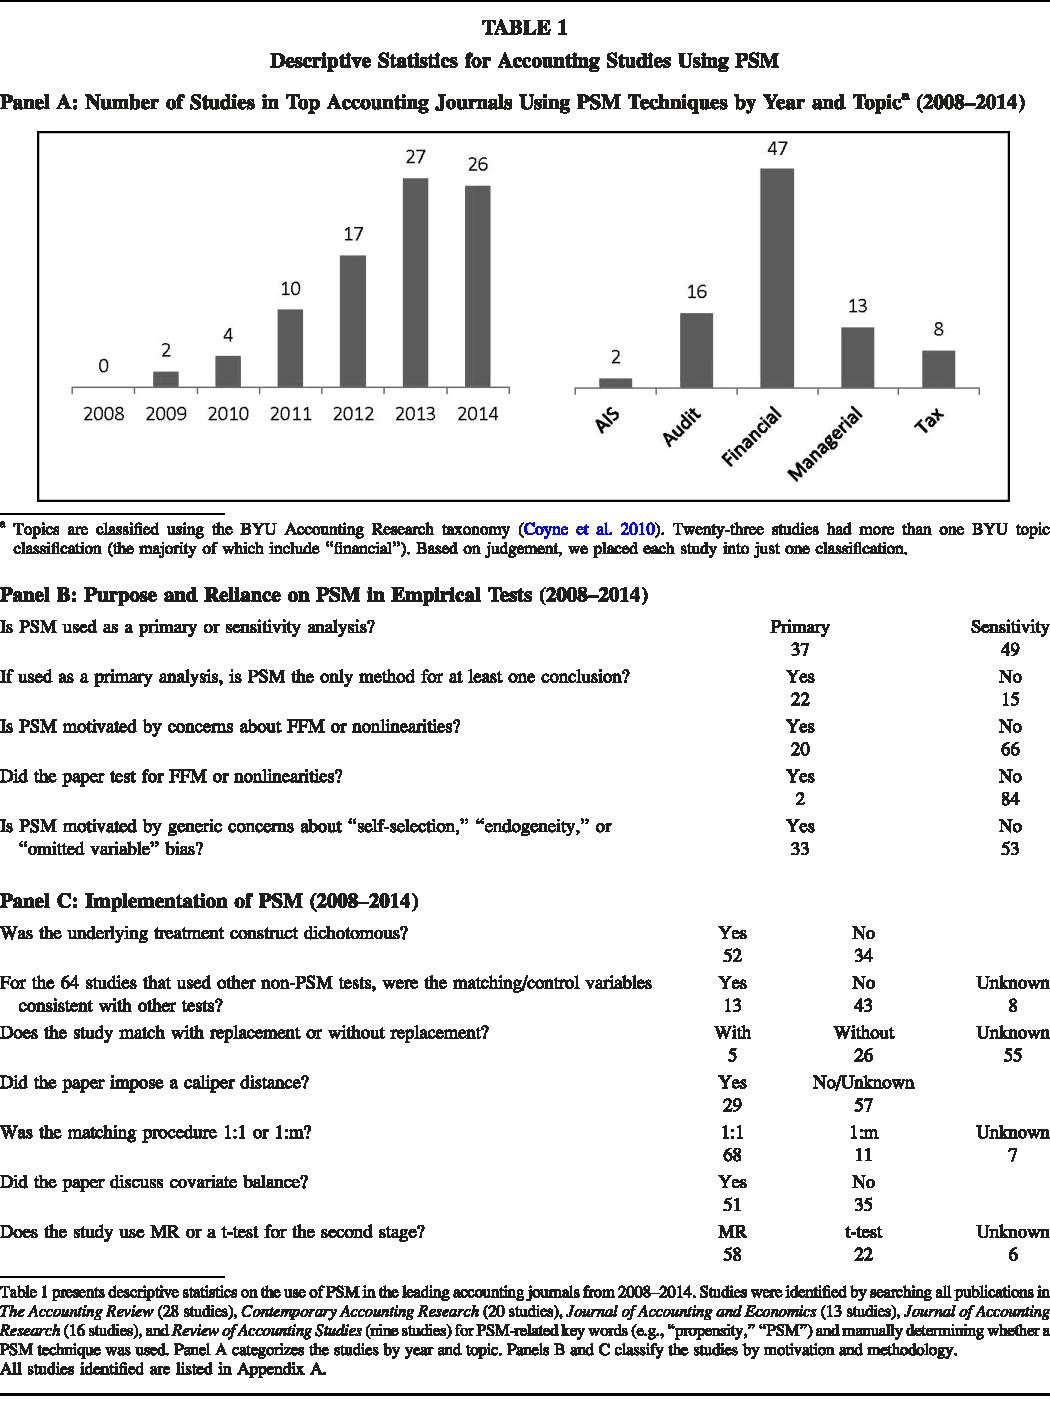
\includegraphics[width=16cm]{../table/tbl01.pdf}
\end{table}

\begin{itemize}
 \item 2008 $\sim$ 2014 年における、\textit{The Accounting Review,
       Contemporary Accounting Research, Journal of Accounting and
       Economics, Journal of Accounting Research, and Review of
       Accounting Studies} に掲載された論文延べ 86 件が対象。
 \item 会計研究で PSM が用いられはじめたのは最近 (86 件中 70 件は 2012
       $\sim$ 2014 の期間に刊行)。
\end{itemize}

\paragraph{各研究の PSM の位置付け (Table 1 Panel B)}

\begin{itemize}
 \item 主要な分析 (primary analyses) として用いている研究が 37 件である
       のに対し、ロバスト・チェック (sensitivity or robustness tests) と
       して用いている研究は 49 件。
 \item PSM を採用する理由として FFM や重回帰分析の線形性の仮定を挙げてい
       る研究はわずか 20 件。
 \item PSM が対処しうる内生性の問題を提示することなく、広く ``自己選択
       (self--selection),'' ``内生性 (endogeneity),'' および ``欠落変数
       バイアス (omitted variable bias)'' への対応として PSM を用いてい
       る研究が 33 件ある。
 \item Heckman (1979) の代わりとして誤用してしまっている研究も存在する。
\end{itemize}

\paragraph{処置群の選択の方法 (Table 1 Panel C)}

\begin{itemize}
 \item 問題の所在
       \begin{itemize}
        \item 処置が 2 値変数 (dichotomous) であるならば、PSM の実施は単純である。
        \item しかしながら、多様な状況でマッチングを実施するため、連続 (あるい
              は順序) 変数に閾値を設けて変換することがある\footnote{2 値
              変数を用いた処置群の選択について、例えば修正再表示のアナウ
              ンスメントや IFRS のアドプションがあげられる。一方で、非 2
              値変数を用いた処置群の選択について、企業の所有構造や監査人
              の産業特殊性 (auditor industry specialization) があげられ
              る}。
       \end{itemize}
 \item 問題点
       \begin{itemize}
        \item このような場合、閾値の近傍の観測値が over--represent される
              傾向があり、それによって、効果の大きさ (および平均処置効果)
              が消失し、第 II 種の過誤が生じる可能性が増大する。
       \end{itemize}
 \item 連続変数を用いている研究の数
       \begin{itemize}
        \item 34 件。また、この影響により、効果の大きさのみならずサンプ
              ル・サイズも低下する。
        \item 59 (12) 件の研究において、MR のサンプル・サイズの大きさは
              PSM の 3 (10) 倍である。
        \item サンプルサイズが小さいほど、サブサンプルは母集団を代表しな
              くなる。
       \end{itemize}
\end{itemize}

\paragraph{コントロール変数の選択 (Table 1 Panel C)}

\begin{itemize}
 \item MR と PSM のいずれを用いるにせよ、同様のコントロール変数を用いる
       べきであるにもかかわらず、しばしば異なるコントロール変数が用いら
       れていることがわかった。
 \item MR からマッチングに用いた変数を除外することは、その変数が処置変数
       (treatment) にも結果変数 (outcome) にも影響を与えないこと、
       ひいては、その変数によるマッチングが不必要であることを意味するに
       他ならない。
 \item 分析においては、\textit{post hoc} なモデルの特定 (model
       specification) をおこなっているという疑念 (appearance; 外観) を避
       けるため、PSM と他のテストとの説明変数の不一致を検討すべきである。
\end{itemize}

\paragraph{傾向スコア推定後のマッチング・プロシージャ (Table 1 Panel C)}

\begin{itemize}
 \item 置換処理 (replace)
       \begin{itemize}
        \item 55 件の研究において、マッチングに際して置換処理がおこなわ
              れているか否か (matching is performed with or without
              replacement) 開示されていない。
        \item 開示している 31 件の研究のうち、5 件が置換あり、26 件が置
              換なしであった。
       \end{itemize}
 \item キャリパー距離 (caliper distance)
       \begin{itemize}
        \item マッチング・プロシージャとしてキャリパー距離を開示して
              いる研究は 29 件のみ。
        \item 開示されているキャリパー距離の分布は、0.00005 から
              0.23 までで、よく用いられている距離は 0.01 (4 件)、0.03 (6
              件)、および 0.10 (5 件) である。
       \end{itemize}
 \item 1 対 1 と 1 対多のどちらのマッチングを用いるか
       \begin{itemize}
        \item 1 対 1 (one--to--one) が 68 instances であるのに対し、1 対
              多 (one--to--many) が 11 instances である。
       \end{itemize}
\end{itemize}

\paragraph{covariate balance (Table 1 Panel C)}

\begin{itemize}
 \item マッチング変数の数 (number of matching variables)、キャリパー距離
       (caliper distance)、グループ・サイズ (group size) などの要因は、
       PSM によってサンプルに covariate balance が生じる程度に影響する。
 \item しかしながら、covariate balance の決定はマッチング・クオリティ
       についての主観的な判断を要求するため、マッチングが実際に適切な
       (sufficient) balance を達成しているか否か、しばしば不透明である。
 \item サーベイの結果、35 件はマッチされたサンプル (matched sample) の
       covariate balance について議論しておらず、4 件のみ傾向スコ
       アの平均差について議論している。
 \item 研究においては、残存した covariate imbalance の効果を緩和するため
       に、PSM のサブサンプルにおいて MR を使うことができる。
 \item サーベイの結果、58 件は (第 2 段階の) ATE を推定する際に MR を用
       いている、22 件は結果変数の距離を t 検定することによって、処置効
       果を推定している、そして、6 件は推定手法を開示していないというこ
       とが明らかとなった。
\end{itemize}

\paragraph{サーベイの結論}

\begin{itemize}
 \item 本節で指摘した問題点は現在の文献でも改善されていない。
 \item Heckman (1979) モデルについて含意を示した Lennox et al. (2012,
       589) の結論と同様に、われわれは、多数の研究が ``重要な計量経済学
       上の問題点および PSM の利用をとりまく問題点に対する理解
       (appreciation) がほとんど無いままに、'' PSM を実施していると結論
       付ける。 
\end{itemize}
\section{EMPIRICAL EXAMPLES OF PROPENSITY SCORE MATICHNG IN ACCOUNTING SETTINGS}
監査法人の規模、内部統制、アナリストのフォロー数が財務報告の質に与える影響を検証する。

\subsection*{Sample Selection and Descriptive Statistics}

\paragraph{サンプルの選択}

\begin{itemize}
 \item 期間は、Sarbanes-Oxley (SOX) 法にかかる観測値が取得可能な2004〜2012年である。
 \item 以下の要件に該当するサンプルを除外する。
   \begin{itemize}
    \item 海外企業、および金融業(2桁SICコードの60--69)に属する観測値
    \item 総資産が500ドル以下の観測値
    \item 2桁SICコードに基づく産業年が10観測値未満のもの(裁量的会計発生高を計算するための要件)
    \item 欠損値のある観測値
   \end{itemize}
 \item 最終サンプルは、監査法人の規模の分析とアナリストのフォローの分析で29,227観測値、内部統制の弱さの分析で20,385観測値である。
 \item 最終サンプルの内訳は、以下のとおりである。
    \begin{itemize}
    \item Big 4に監査されている($\mathit{BIG}4_{it}=1$)のが19,988企業年
    \item 少なくとも1つの内部統制の弱さを監査報告書で指摘されている($\mathit{WEAK}_{it}=1$)のが1,422企業年
    \item 少なくとも1人のアナリストがついている($\mathit{ANALYST}_{it}=1$)21,144企業年
   \end{itemize}
\end{itemize}

\paragraph{データソース}

\begin{itemize}
 \item 監査法人、内部統制の弱さ、財務諸表の再報告にかかるデータ:Audit Analytics
 \item アナリストにかかるデータ:the Institutional Brokers’ Estimate System (I/B/E/S)
 \item 財務データ:Compustat
  \begin{itemize}
   \item Table 2:記述統計量
  \end{itemize}
\end{itemize}

\subsection*{Research Design}

$\mathit{BIG}4_{it}$、$\mathit{WEAK}_{it}$、$\mathit{ANALYST}_{it}$のそれぞれを割り当て変数とし、PSMを行い、ATEを推定する。

\paragraph{予測モデル(第1段階)}

\begin{equation}
\mathit{D}_{it} = \alpha_0 + \alpha_1 \mathit{X}_{it} + \varepsilon_{it}
\end{equation}

\begin{itemize}
 \item $\mathit{D}_{it}$は、$\mathit{BIG}4_{it}$、$\mathit{WEAK}_{it}$、$\mathit{ANALYST}_{it}$で、処置群と対照群に割り当てるダミー変数
 \item PSMのキャリパー距離は、0.03とする。
\end{itemize}

\paragraph{結果モデル(第2段階)}

\begin{equation}
\mathit{QUALITY}_{it} = \beta_0 + \beta_1 \mathit{D}_{it} + \beta_2 \mathit{X}_{it} +\varepsilon_{it}
\end{equation}

\begin{itemize}
 \item $\mathit{QUALITY}_{it}$は、財務報告の質を示し、本分析では、裁量的会計発生高($\mathit{ABSACC}_{it}$)、および財務諸表の再報告($\mathit{RESTATE}_{it}$)のそれぞれで評価している。
 \item $X_{it}$は、企業規模($\mathit{LNASSETS}_{it}$)、パフォーマンス($\mathit{ROA}_{it}$、$\mathit{ATURN}_{it}$)、財政状態($\mathit{CURR}_{it}$、$\mathit{LEV}_{it}$、$\mathit{DISTRESS}_{it}$)、設立年数($\mathit{AGE}_{it}$)、成長性($\mathit{GROWTH}_{it}$)、企業価値($\mathit{BTM}_{it}$)、年度固定効果を用いる。
  \begin{itemize}
   \item Appendix B:変数の定義
  \end{itemize}
 \item 本分析で観察したいATEは、(5)式の$\beta_1$で示される。
\end{itemize}

\subsection*{Diagnosing Function Form Misspecification}
\begin{itemize}
 \item MRにおいて、FFMが懸念されるのかについて判定する。
 \item Ramsey(1969)のRESETテストがFFMを見る手法として用いられることがある(Lawrence et al. 2011を見よ)。
 \item ただし、これは、変数の非線形性が追加的な説明を与えているのかどうかについて検証するものであり、結果変数と非線形な関係にある変数がATEの推定にバイアスを与えてるのかどうかを見るものではない。
\end{itemize}

\paragraph{変数を追加してFFMを判定する方法(Table 3)}

\begin{itemize}
 \item ここで、MRにおけるFFMを判定する手法として、コントロール変数(たとえば、変数を2乗したもの、3乗したもの)を追加する手法を提唱する。
 \item もし、元のモデルと変数を追加したモデルの結果が異なるのなら、FFMに対する懸念がある。
 \item (5)式を推定した結果を見ると、変数を追加したとしても((2)列と(5)列)、基本的な結果は元のモデル((1)列と(4)列)大きくは変わらない。
 \item しかし、監査法人の規模とアナリストのフォローで割り当てた場合、Chow(1960)の検定をすると、元のモデルのATEと変数を追加したモデルのATEの間で有意な差が認められる。
  \begin{itemize}
   \item これは、$X$と結果変数が非線形な関係にあることを示す。
  \end{itemize}
\end{itemize}

\subsection*{First-Stage Prediction Model}

\paragraph{第1段階((4)式)の推定結果(Table 4)}

\begin{itemize}
 \item 先行研究では、pseudo-${\rm R^2}$が高ければ高いほど、PSMは良い状態であることが示唆されている。
 \item しかし、この説明力は、割り当てが大きく影響を与えている。
 \item つまり、処置群の$X$が対照群の$X$とより大きく相違しているのなら、回帰式の説明力は大きくなる。
 \item overlapが大きければ大きいほど、pseudo-${\rm R^2}$は小さくなるとも言える。
  \begin{itemize}
   \item ただし、説明力がPSMの有効性を必ずしも示しているわけではない。
  \end{itemize}
\end{itemize}

\subsection*{Demonstration of Propensity Score Overlap}

処置群と対照群の傾向スコアのoverlapについて確認するため、Shaikh, Simonsen, Vydacil, and Yildiz(2009)と同様に、傾向スコアの密度をプロットする。

\paragraph{監査法人の規模で割り当てた場合の傾向スコアのプロット(Figure 1, Panel A)}

\begin{figure}
 \centering
 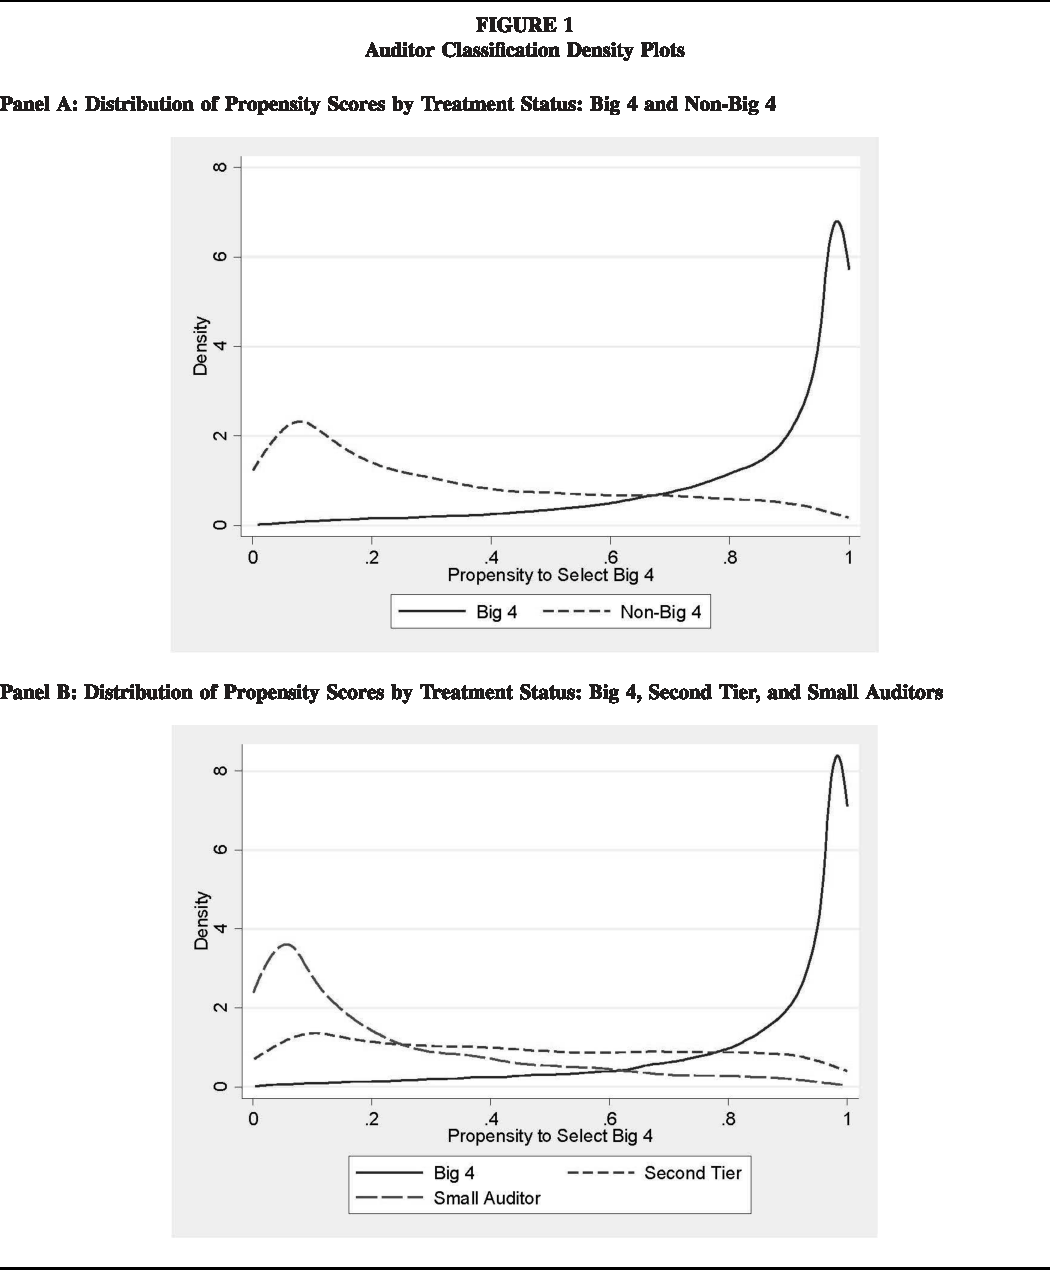
\includegraphics[width=16cm]{../fig/fig01.pdf}
\end{figure}

\begin{itemize}
 \item Big 4の監査法人のクライアントの傾向スコアは、0.9〜1の範囲内に集中し、非Big 4の監査法人のクライアントの傾向スコアは、0〜0.2に集中している。
 \item これは、共変量が割り当ての決定に大きく影響していることを示している。
 \item 結果的に、マッチングは、主として極端でない傾向スコアの範囲(ここでは、0.2〜0.9)の範囲内でなされることになる。
\end{itemize}

\paragraph{Second Tierを考慮して割り当てた場合の傾向スコアのプロット(Figure 1, Panel B)}

\begin{itemize}
 \item 非Big 4のクライアントから、Second Tierの監査法人のクライアントを識別する。
 \item この識別をしたプロットを見ると、Second Tierのクライアントは、0〜0.2の範囲内で、小規模監査法人のクライアントよりも傾向スコアが小さいが、0.2以上では小規模監査法人よりも大きな傾向スコアであることがわかる。
 \item これは、Second TierのクライアントがBig 4のクライアントとより多くマッチングが成立することを示す。
\end{itemize}

\paragraph{内部統制の弱さで割り当てた場合の傾向スコアの密度のプロット(Figure 2, Panel A)}

\begin{figure}
 \centering
 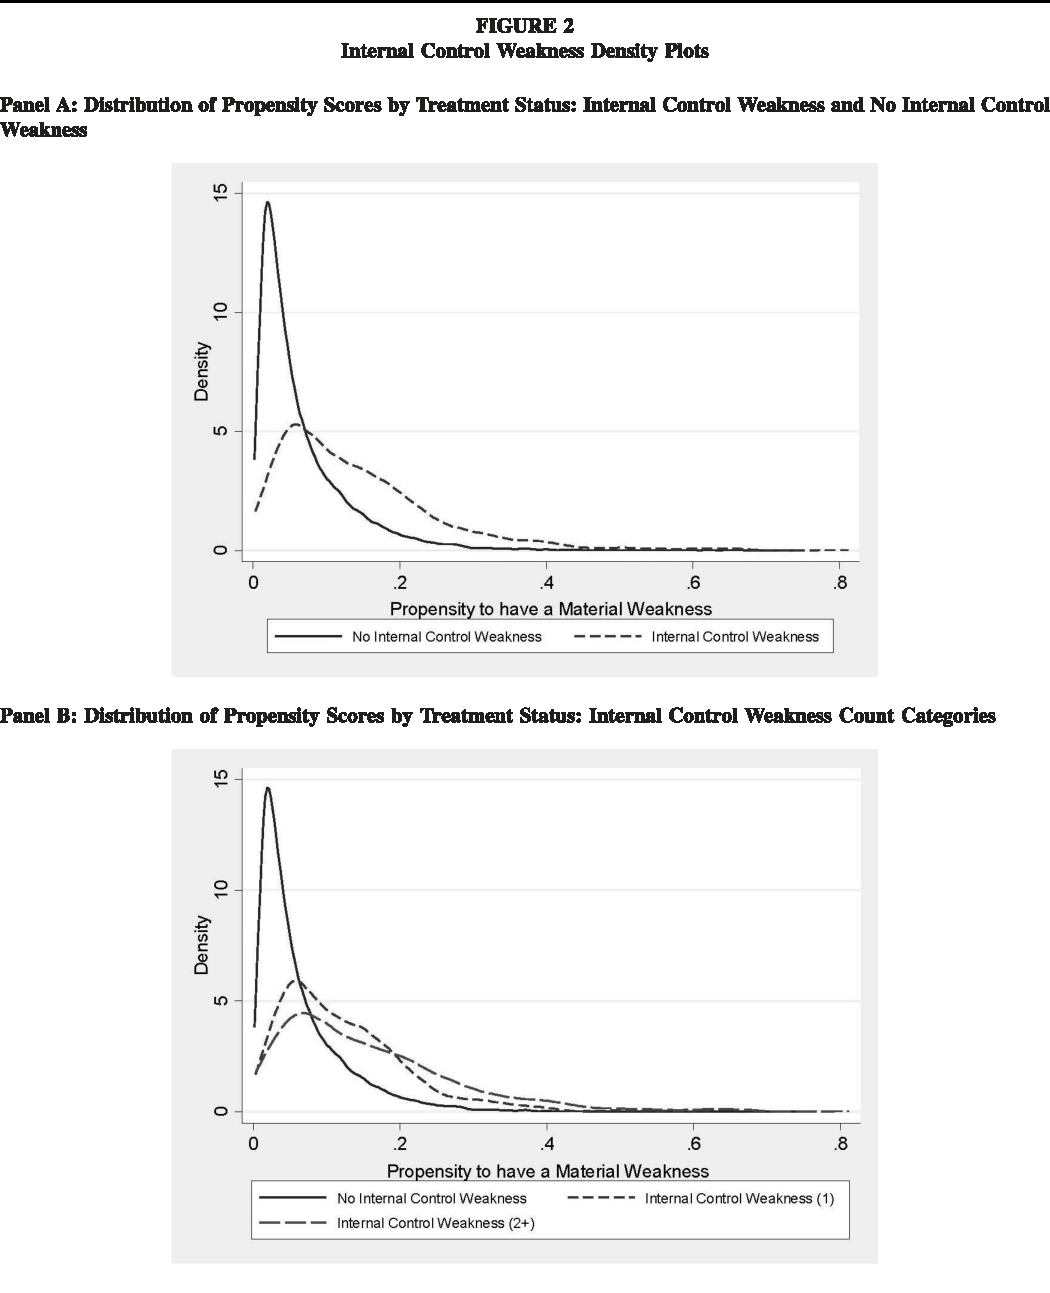
\includegraphics[width=16cm]{../fig/fig02.pdf}
\end{figure}

\begin{itemize}
 \item 監査法人の規模のときよりも、overlapの範囲が大きいことがわかる。
 \item Table 4のpseudo-${\rm R^2}$も、低い値であることもこのことを示唆している。
\end{itemize}

\paragraph{内部統制の弱さの判定を詳細にした場合の傾向スコアの密度のプロット(Figure 2, Panel B)}

\begin{itemize}
 \item 内部統制の弱さの判定をより詳細にする(No ICW、1 ICW、2+ICW)。
 \item 監査法人の規模の場合と同様に、overlapは、No ICWと2+ICWの間よりも、No ICWと1 ICWの間の方がより大きいことがわかる。
\end{itemize}

\paragraph{アナリストのフォローで割り当てた場合の傾向スコアの密度のプロット(Figure 3, Panel A)}

\begin{itemize}
 \item 監査法人の場合と同様に、処置群と対照群との間で傾向スコアの密度の範囲は異なっており、overlapが限定的なものであることがわかる。
\end{itemize}

\paragraph{アナリストのフォロー数を詳細にした場合の傾向スコアの密度のプロット(Figure 3, Panel B)}

\begin{itemize}
 \item アナリストのフォロー数を詳細にみる(1〜5人、6〜10人、11人以上)。
 \item プロットした結果、アナリストの数が少なければ少ないほど、アナリストに全くフォローされてない観測値とのoverlapが大きくなることがわかる。
 \item これは、マッチングがフォローしているアナリストの数の少ない企業となされる可能性が高いことを示している。
\end{itemize}

\subsection*{Matching without Replacement}

置き換えを認めず、1対1でマッチングを行う。

\paragraph{サンプルの構成(Table 5, Panel A)}

\begin{itemize}
 \item 置き換えをせず1対1でマッチングすると、かなりの数の観測値を除去することになる。
 \item 事実、“full sample”を比較して、監査法人の規模で30\%、内部統制の弱さで14\%、アナリストのフォローで28\%のサンプルしか確保できなかった。
 \item また、マッチングしたサンプルは、Second Tierのクライアントや、アナリストのフォロー数が少ない観測値で構成されていることもわかる。
  \begin{itemize}
   \item サンプルが小さいことは、外的な妥当性を減少させる、もしくは欠落させてしまう可能性を有している。
  \end{itemize}
\end{itemize}

\paragraph{MRとPSM間における共変量とATEの比較(Table 5, Panel B)}

\begin{itemize}
 \item 共変量は、PSMを行うことにより、バランスが向上していることがわかる。
  \begin{itemize}
   \item これは、MRにおいて、処置群と対照群の相違が残ったまま、ATEを推定していることを示す。
  \end{itemize}
 \item 裁量的会計発生高を従属変数とした場合、MRのATEはすべて有意であるが、PSMはすべて非有意であり、Chow(1960)の検定も、すべての係数間で有意である。
 \item 一方、財務諸表の再報告を従属変数とした場合は、MRとPSMのATEともにすべて類似した結果を示すが、係数を比較すると、有意な差が検出されるものが存在している。
\end{itemize}

\paragraph{まとめ}
\begin{itemize}
 \item 以上の分析から、MRとPSMでは推定される ATEが有意に異なっていることが明らかとなった。
 \item もし、PSMのみで分析すると、監査法人の規模、内部統制の弱さ、およびアナリストのフォローは、財務報告の質に影響を与えていないという結果のみを得ることになる。
 \item しかし、この ``帰無仮説を採択する'' (accept the null hypothesis) のは結論を急ぎ過ぎ (premature) であるかもしれない。
 \item 以下で、PSMの手法を変更することで、結果が変化することを示す。
\end{itemize}

\subsection*{Matching with Replacement}

置き換えを認めて、1対1でマッチングを行う。

\paragraph{サンプルの構成(Table 6, Panel B)}

\begin{itemize}
 \item (2)列目は、サンプルサイズが小さい方の群を処置群とし、サンプルサイズの大きな方の群にマッチングの置き換えを認める場合の結果である(Panel A)。
 \item サンプルサイズが大きくなっており、キャリパー距離(0.03)の間でより多くの対照群の観測値がマッチングしていることがわかる。
 \item (3)列目は、サンプルサイズの大きな方の群を処置群とし、サンプルサイズの小さい方の群にマッチングの置き換えを認める場合の結果である。
 \item サンプルサイズがかなり大きくなっており、ウェイトがいずれも5以上であることから、対照群の観測値がより多くの回数マッチングしていることがわかる。
 \item マッチングの手法ごとにサンプルの構成を比較した結果、9個の比較中8個で有意な差が認められる。
 \item 特に、Second Tierのクライアントの割合と、アナリストのフォロー数の平均値は、マッチングの手法間で顕著な差がある。
  \begin{itemize}
   \item マッチング手法の違いが、サンプルサイズとサンプルの構成に影響を与えてしまうことが示唆されている。
  \end{itemize}
\end{itemize}

\paragraph{ATEの比較(Table 6, Panel B, C)}

\begin{itemize}
 \item 監査法人の規模で割り当てた場合の結果は、いずれも非有意である。
 \item しかし、ATEの差が有意に検出されているものが存在する(6個の比較中3個)。
 \item 内部統制の弱さ、およびアナリストのフォローで割り当てた場合の結果は、マッチングの手法ごとに異なっており、ATEの差も有意に検出されているものがある(12個の比較中7個)。
  \begin{itemize}
   \item マッチングの手法が統計的な結果に影響を与えてしまう。
  \end{itemize}
\end{itemize}

\subsection*{The Influence of Matching Variables on Estimates of the ATE}

\paragraph{変数を置き換えてマッチングを行なった場合のサンプルの構成(Table 7, Panel A)}

\begin{itemize}
 \item 企業規模を示す変数を、総資産の自然対数($\mathit{LNASSETS}_{it}$)から時価総額の自然対数($\mathit{LNMARKET}_{it}$)に入れ替える。
 \item マッチングの手法間でサンプルを比較すると、共通の観測値は、58.9〜71.4\%の割合である。
 \item さらに、内部統制の弱さで割り当てた場合の対照群(内部統制の弱さが指摘されていない観測値)は、マッチングの手法間で、わずか18.2\%しかサンプルが共通してない。
\end{itemize}

\paragraph{変数を置き換えてマッチングを行なった場合のATE(Table 7, Panel B)}

\begin{itemize}
 \item $\mathit{LNASSETS}_{it}$のATEよりも、$\mathit{LNMARKET}_{it}$のATEの方が、有意であるものが多いことがわかる。
 \item 特に、アナリストのフォローで割り当てとし、財務諸表の再報告を従属変数とした時のATEは、Table 5の全サンプルとマッチングサンプルで非有意だったにもかかわらず、変数を置き換えると有意な結果が確認される。
 \item Chow(1960)の検定によれば、6個の比較中、3個でATEが有意な差であることが確認される。
\end{itemize}

\paragraph{変数を追加してマッチングを行った場合の結果(Table 8)}

\begin{itemize}
 \item 以下のとおり、変数を追加してマッチングを行う。
  \begin{itemize}
   \item 監査法人の規模:営業活動にかかるキャッシュフロー($\mathit{CFO}_{it}$)、海外売上高($\mathit{FOREIGN}_{it}$)
   \item 内部統制の弱さ:損失ダミー($\mathit{LOSS}_{it}$)
   \item アナリストのフォロー:$\mathit{LNMARKET}_{it}$
  \end{itemize}
 \item このマッチングからATEを求めた結果は、(2)列目と(5)列目に示されているが、いずれも有意であることがわかる。
 \item さらに以下のとおり変数を追加する。
  \begin{itemize}
   \item 監査法人の規模:$\mathit{LNASSETS}_{it-1}$、$LOSS_{it}$、棚卸資産($\mathit{INVENTORY}_{it}$)
   \item 内部統制の弱さ:$\mathit{FOREIGN}_{it}$
   \item アナリストのフォロー:$\mathit{BTM}_{it-1}$
  \end{itemize}
 \item 以上でマッチングし、ATEを求めた結果は、(3)列目と(6)列目に示されているが、これまでの検証で一貫して有意である内部統制の弱さで割り当て、財務諸表の再報告を従属変数としたATE以外、すべて非有意である。
  \begin{itemize}
   \item 以上から、ATEの推定は、PSMのモデルの設定から影響を受けやすいことが明らかである。
  \end{itemize}
 \item 以上の変数の選択は、結果の頑健性を示すために、``事後的''に選択されたことに留意するべきである。
 \item すべての$X$は、結果に同じような影響を与えるとは限らない。
  \begin{itemize}
   \item ここから、PSMの変数の選択において、十分な考慮をするこの重要さが示唆される。
  \end{itemize}
\end{itemize}

\section{Suggestions and consideration for future research}
\paragraph{本節の検討内容}
\begin{itemize}
 \item 内生性問題に対する``特効薬''は存在しないため、
       あらゆる方法で慎重に検討する必要がある。
 \item PSMは、観測不可能な要因を選択する上での内生性を特定するものではないが、
       FFMに関する内生性については、有用であると考えられる。
 \item 本節では、PSMを利用する上でより説得力を高めるための提言と、
       PSMを利用した分析結果を評価する際に検討すべき事項について述べる。
\end{itemize}

\subsection{Suggestions for improved application of propensity score matching}
\paragraph{PSMの利用を検討している研究に対する提言}
\begin{enumerate}
 \item FFMに関する識別問題に取り組むための手段としてPSMを利用すべきあり、PSMが
       ``内生性''``自己選択''``欠落変数バイアス''に関する一般的な懸念事項を緩和すると
       示唆するのは避けるべきである。
 \item PSMを利用した単一の (もしくは小数の) の結果だけをもとに、推論を行うべきではない。
       \begin{itemize}
        \item ``マッチング手法は回帰の修正 (regression adjustment) と
              対立するものではないと認識されるべきであり、実際、その2つの手法は補完的であり、
              組み合わせて使用することが望ましい。'' (Stuart, 2010, 2)
       \end{itemize}
 \item PSMとMRの両方を利用する場合、
       PSMのマッチング段階において、MRから除かれる変数を含めるべきではない。
       \begin{itemize}
        \item MRで除かれる変数についてマッチングを行うことで、
              MRとPSMが不均一 (unequal) になり、一方もしくは両者の特性 (specifications) に
              疑問が生じることになる。
        \item PSMの第2段階において、
              全てのコントロール変数を含めてMRを推定した場合の処置効果を推定すべき (``二重にロバストな推定'' (``doubly robust''estimation))
       \end{itemize}
 \item リサーチ・デザインの再現可能性と明瞭性を高めるために、
       PSMの設定を開示すべきである。具体的な内容は以下の通りである。
       \begin{enumerate}
        \item 傾向スコアを推定するためのモデル (第1段階)
        \item ATEを推定するためのモデル (第2段階)
        \item マッチング手法によって観測値を置き替えるか否か
        \item 処置済みの各観測値 (treated observation) に対して、マッチさせたコントロールの観測値数
        \item (実施する場合、) キャリパー距離 (caliper distance)
        \item マッチングの質 (共変量のバランス (covariate balance))
       \end{enumerate}
\end{enumerate}

\subsection{Considerations when using propensity score matching}
\paragraph{PSMを利用している場合の検討事項}
\begin{enumerate}
 \item 処置特性 (treatment specification) に関する検討
       \begin{itemize}
        \item 適切なマッチングの数が十分に存在している場合、
              効果量が最大となるような、母集団から抽出した部分集合に焦点をあてるために、
              ``最大限の''処置を施された観測値を``最小限の''処置を施された観測値に
              マッチさせることを、代替的手法として推奨する。
       \end{itemize}
 \item マッチング変数と処置効果の関係に関する検討
       \begin{itemize}
        \item treatmentの選択を決定する性質も、因果効果 (the effect of treatment) に関連している
              可能性がある。
        \item 機械的に、``最大の''因果効果を持つ観測値を選択し、また、``最小の''効果を維持させることで、
              PSMはバイアスのかかった推定 (inference) を実施することになる (Heckman et al., 1998)。
       \end{itemize}
 \item 代替的なマッチング設定 (design choiced) が同様の結果を生みだすか否かの検討
       \begin{itemize}
        \item DeFond et al. (2015) は、PSMの設定を無作為に実施し、
              証拠が誤りである可能性の評価についても明記している。
       \end{itemize}
\end{enumerate}

\subsection{Alternatives to propensity score matching for alleviating functional form misspecification}
\begin{itemize}
 \item 以下の方法を実施することで、common supportの範囲外の観測値に関するFFMを緩和することができる一方で、
       PSMにおける裁量性と標本分散の一部を排除することができる。
       \begin{enumerate}
        \item 重複を制限するうえで有効な要因 (例. 企業規模、収益性) を特定し、common supportに該当するサンプルを制限する。
        \item 傾向スコアを推定し、そのスコアが、[$\alpha$, $1-\alpha$] (ただし、$\alpha$は、
              客観的に決定されるcutoff point (例えば、0.10)) の範囲外となるような極端な値をとるサンプルを除く (Crump, Hotz, Imbens and Mitnik 2009)。
       \end{enumerate}
 \item その他にも様々な対処法があるが、どちらか一方を代替するのではなく、FFMを緩和するために補完しあうものである。
 \item PSMで得た結果の頑健性の確認 (stress testing) こそ重要であり、
       証拠の妥当性に対する信頼性を向上させる。
\end{itemize}

% \section{Suggestions and consideration for future research}
% \paragraph{PSMの利用を検討している研究に対する提言}
% \begin{itemize}
%  \item 内生性問題に対する``特効薬''は存在しない。
%  \item 研究者は、適切なリサーチ・デザインを選択する際に、
%        内生性問題についてあらゆる方法で慎重に検討する必要がある。
%  \item 前述のとおり、PSMは観測不可能な要因の選択に関する内生性を特定するものではない。
%  \item ただし、FFMに関する内生性については、有用である可能性がある。
%  \item PSMを利用する上でより説得力のあるものにするための提言と、
%        PSMを利用した結果を評価する際に検討する事項について述べる。
% \end{itemize}

% \subsection{Suggestions for improved application of propensity score matching}
% \begin{enumerate}
%  \item FFMに関する識別問題に取り組むための手段としてPSMを利用すべきあり、PSMが
%        ``内因性''``自己選択''``欠落変数バイアス''に関する一般的な懸念事項を緩和すると
%        示唆するのは避けるべきである。
%  \item 一般に、PSMとMRを組みあわせて使用する場合には慎重になった方が良いと考えられる。
%        Stuart (2010, 2) によると、``マッチング手法は回帰の修正 (regression adjustment) と
%        対立するものではないと認識されるべきであり、実際、その2つの手法は補完的であり、
%        組み合わせて使用することが望ましい。''と指摘されている。
%        このように、PSMを利用した単一の (もしくは小数の) の結果だけをもとに
%        推論を行う前に、慎重に検討した方がよい。
%  \item PSMとMRの両方を利用する場合、
%        PSMのマッチング段階において、MRから除かれる変数を含めることは
%        やめた方が良い。
%        MRにおいて除かれる変数についてマッチングを行うことで、
%        MRとPSMが不均一 (unequal) になり、一方もしくは両者の特性 (specifications) に
%        疑問が生じることになる。同様に、PSMの第2段階において、
%        全てのコントロール変数 (``二重の頑健性''チェック (``doubly robust''estimation)) を
%        含めて、MRを推定した場合の処置効果を推定すべきである。
%  \item リサーチ・デザインの再現可能性と明瞭性に役立てるために、
%        PSMの研究上の設定を開示すべきである。具体的な内容は以下の通りである。
%        \begin{enumerate}
%         \item 傾向スコアを推定するためのモデル (第1段階)
%         \item ATEを推定するためのモデル (第2段階)
%         \item マッチング手法によって観測値を置き替えるか否か
%         \item 処置済みの各観測値に対して、マッチさせたコントロールの観測値数
%         \item (実施する場合には、) キャリパー距離 (caliper distance)
%         \item マッチングの質 (共変量のbalance)
%        \end{enumerate}
% \end{enumerate}

% \subsection{Considerations when using propensity score matching}
% \begin{enumerate}
%  \item 処置特性 (treatment specification) に関する検討
%        \begin{itemize}
%         \item continuous constructの水準に基づいて因果を検証した場合、
%               PSMはcutoff周辺の観測値と優先的させる傾向がある。
%         \item この場合、マッチしたサンプルから得られた結果を母集団に一般化できるか
%               かどうかを検討しなければならない。
%         \item 適切なマッチングの数が十分に存在している場合、
%               効果量が最大となるような、母集団から抽出した部分集合に焦点をあてるために、
%               ``最大限の''処置を施された観測値を``最小限の''処置を施された観測値に
%               マッチさせることを、代替的手法として推奨する。
%        \end{itemize}
%  \item マッチング変数と処置効果の関係に関する検討
%        \begin{itemize}
%         \item treatmentの選択を決定する性質も、因果効果 (the effect of treatment) に関連している
%               可能性がある。
%         \item 例えば、規模の大きいクライアントは、
%               小規模な監査人よりも4大監査法人から得られるベネフィットが多いと想定する。
%         \item 規模の大きいクライアントは、
%               合理的な反実仮想 (counterfactuals) 
%               (規模の大きいクライアントが小規模な監査人から得られるベネフィットは、
%               4大監査法人から得られるベネフィットよりも大きい)  
%               を有するとは考えられないため、PSMはそれらを放棄する。
%         \item この場合、マッチしたサンプルから得られるthe likelihood of exclusion (除外される傾向?)
%               は、因果効果と関連する。
%         \item 機械的に、``最大の''因果効果を持つ観測値を選択し、また、``最小の''効果を維持させることで、
%               PSMはバイアスのかかった推定 (inference) を実施することになる (Heckman et al., 1998)。
%        \end{itemize}
%  \item 代替的なマッチング設定 (design choiced) が同様の結果を生みだすか否かの検討
%        \begin{itemize}
%         \item 代替的なリサーチ・デザインを推定するためにPSMを利用する際には、
%               慎重になる必要がある。
%               この点について、DeFond et al. (2015) は、PSMの設定を無作為に実施し、
%               証拠が誤りである可能性の評価についても明記している。
%        \end{itemize}
% \end{enumerate}

% \subsection{Alternatives to propensity score matching for alleviating functional form misspecification}
% \begin{itemize}
%  \item 以下の方法を実施することで、common supportの範囲外の観測値に関するFFMを緩和することができる一方で、
%        PSMにおける裁量性と標本分散の一部を排除することができる。
%        \begin{enumerate}
%         \item 重複を制限するうえで有効な要因 (例. 企業規模、収益性) を特定し、common supportに該当するサンプルを制限する
%         \item 傾向スコアを推定し、そのスコアが、[$\alpha$, $1-\alpha$] (ただし、$\alpha$は、
%               客観的に決定されるcutoff point (例えば、0.10)) の範囲外となるような極端な値をとるサンプルを除く (Crump, Hotz, Imbens and Mitnik 2009)。
%        \end{enumerate}
%  \item その他にも様々な対処法があるが、どちらか一方を代替するのではなく、FFMを緩和するために補完しあうものである。
%  \item PSMで得た結果の頑健性の確認 (stress testing) こそ重要であり、
%        証拠の妥当性に対する信頼性を向上させる。
% \end{itemize}

\section{CONCLUSION}

\begin{itemize}
 \item Shipman, Swanquist, and Whited の分析対象
       \begin{itemize}
        \item PSM の理論的基礎を議論し、昨今の会計研究における PSM の利
              用を調査し、そして、デザインの選択 (design choice) にかん
              する実践的なインプリケーションを例示した。
       \end{itemize}
 \item 会計研究における PSM の利用 (第 3 節) の要約
       \begin{itemize}
        \item 観察不能なデータによって生じる内生性を緩和するための
              Heckman (1979) モデルの代わりとして、誤って利用しているケー
              スがしばしば確認される。
        \item デザインの選択を開示していない、あるいは、PSM と MR とでコ
              ントロール変数が不一致である研究が散見される。
       \end{itemize}
 \item デザインの選択 (第 4 節) の要約
       \begin{itemize}
        \item カットオフ・ポイント (cutoff point) が処置群を決定する場合、
              カットオフの近傍の観測値は over--represent し、第 II 種の
              過誤が生じる可能性が増大する。
        \item PSM による推定は変化しやすく (fickle) リプリケートが難しい
              ため、マッチド・サンプルに対して ``ストレス・テスト''
              (stress testing) を実施し、また、代替的なリサーチ・デザイ
              ンで PSM の追加検証を実施することが要求される。
       \end{itemize}
 \item 将来研究への提言
       \begin{itemize}
        \item 重要なデザインの選択を開示すること。
        \item PSM の利用目的を適切に理解すること。
        \item マッチド・サンプル以外の specification concerns も調査する
              こと。
        \item PSM に対して他のリサーチ・デザインをもとに追加分析を実施す
              ること、および、FFM に対処する新たな手法を模索すること。
       \end{itemize}
\end{itemize}
\appendix
\setcounter{section}{1}
\section{Appendix B}
\begin{longtable}[c]{ll}
 \caption{Variable Descriptions}
 \label{tab:appB}
 \\
 % -- ページの表の最上部 --
 \hline
  Variable Name & \hspace{5cm} Variable Definition \\ \hline
 \endhead
 % -- ページの表の最下部 --
 \hline
 \endfoot
 % ------------------------
  $\text{ABSACC}_{it}$ & 全ての産業--年度において最低10個の観測値をもとに以下の回帰式を推定し、\\
  & 得られた誤差を業績とマッチさせて算定した裁量的会計発生高 \vspace{0.5cm} \\
  \vspace{0.3cm}
  & {$\!
      \begin{aligned}
     \frac{TA}{A} = \alpha + \lambda_{0} 
       \frac{1}{A} + \lambda_{1} \frac{\Delta REV - \Delta REC}{A} 
       + \lambda_{2}\frac{PPE}{A}
      \end{aligned} $} \\
  & \begin{tabular}{ll} \hline
     $A$ & 総資産の平均値 \\
     $\text{TA}$ & 総会計発生高 (= 経常利益 - 営業活動によるキャッシュ・フロー) \\
     $\Delta REV$ & 売上高の変化額 \\
     $\Delta REC$ & 売上債権の変化額 \\
     $PPE$ & 有形固定資産 \\ \hline
    \end{tabular} \vspace{0.3cm} \\ 
  & 上記の回帰式から得られた各観測値の誤差を、\\
  & 同じSIC (two-digit) コードでROAが最も近似している観測値から引いた絶対値を \\
  & $\text{ABSACC}$ としている。\\
  $\text{ANALYST}_{it}$ & 1人以上のアナリストがフォローしている企業であれば1、\\
  & そうでなければ0を与えるダミー変数 \\
  $\text{AGE}_{it}$ & t年時点でCompustatに収録されている企業年数 \\
  $\text{ATURN}_{it}$ & 売上高÷総資産の平均値 \\
  $\text{BIG4}_{it}$ & 監査人が4大監査法人であれば1、そうでなければ0を与えるダミー変数\\
  $\text{BTM}_{it}$ & 簿価時価比率 \\
  $\text{CFO}_{it}$ & 営業活動によるキャッシュ・フロー÷総資産額の平均値\\
  $\text{CURR}_{it}$ & 流動比率\\
  $\text{DISTRESS}_{it}$ & Altman (1983) に基づいて算定したZスコア\\
  & {$\!
      \begin{aligned}
       0.717 \times \frac{\text{運転資本}}{\text{総資産}} &+ 0.847 \times \frac{\text{留保利益}}{\text{総資産}} 
       + 3.107 \times \frac{\text{利息・税控除前利益}}{\text{総資産}} \\
       &+ 0.42 \times \frac{\text{自己資本簿価}}{\text{総負債}}
       + 0.998 \times \frac{\text{売上高}}{\text{総資産}}
      \end{aligned} $} \\
  $\text{FOREIGN}_{it}$ & 外国為替損益が0でなければ1、そうでなければ0を与えるダミー変数 \\
  $\text{GROWTH}_{it}$ & t-1期からt期への売上高の変化額÷t-1時点の売上高 \\
  $\text{INVENTORY}_{it}$ & 棚卸資産÷総資産\\
  $\text{LEV}_{it}$ & 長期借入金 (long-term debt) と短期借入金の合計額÷総資産 \\
  $\text{LNASSETS}_{it}$ & 総資産額 (単位: 100万) の自然対数 \\
  $\text{LNMARKET}_{it}$ & 時価総額 (単位: 100万) の自然対数 \\
  $\text{LOSS}_{it}$ & operating income after depreciationが\\ 
  & マイナスであれば1、そうでなければ0を与えるダミー変数 \\
  $\text{RESTATE}_{it}$ & t期の財務諸表について、後に訂正財務諸表を提出していれば1、\\
  & そうでなければ0を与えるダミー変数 \\
  $\text{ROA}_{it}$ & 当期純利益÷総資産の平均値\\
  $\text{WEAK}_{it}$ & 監査報告書において、内部統制に関する脆弱性が1点以上指摘されていれば1、\\
  & そうでなければ0を与えるダミー変数\\ 
\end{longtable}
\bibliography{./bib/myrefs}
\end{document}
tclass[10pt,uplatex,dvipdfmx]{jsarticle} %times new roman
\usepackage{ascmac}	% required for `\itembox' (yatex added)
\usepackage{amsmath}    % \dfrac 等の数式内の関数を使用する際に必要
\usepackage{graphicx}   % graphicx Excel から図を入れたいときは、
                        % \special{pdf:minorversion=6}
                        % Excel から pdf をとりこみたい場合、"pdfcrop"
                        % をかましておくと余白が効率化される
\usepackage{tikz}
\usepackage{ulem}       % \uline (下線) \uuline (二重下線) を使用する際に必要
\usepackage{natbib}     % jecon を使用する際に必要
\usepackage{bm}         % ベクトルを表記する際に必要
\usepackage{threeparttable} % 表注; includegraphics する場合は
                            % threeparttable 環境を minipage 環境にいれ
\usepackage{newtxtext,newtxmath}        % 数式を Times フォントに変更する
\usepackage{url}
\usepackage{lscape,rotating}    % sideways 環境でその部分だけ rotate。
                                % caption もまとめて rotate したい場合は
                                % sidewaystable 環境もしくは
                                % sidewaysfigure 環境を用いる
\usepackage{dcolumn}
\usepackage{longtable}
\usepackage{booktabs}
\usepackage{pxrubrica}          % \ruby[オプション]{親文字}{ルビ文字}
\usepackage{fancyhdr}
\pagestyle{fancy}

\rhead{担当: 井上謙仁・久多里桐子・大洲裕司}
\lhead{PATW@北海道情報大学 \\ 2017年8月25日 (金)}

% \rhead{井上謙仁・久多里桐子・大洲裕司}
% \lhead{PATW 於 北海道情報大学 (2017--08--25)}
\begin{document}
% \renewcommand{\rmdefault}{ptm}	%{\rmfamily ...} または \textrm を Times に
\bibliographystyle{./bib/jecon}
\title{Propensity Score Matching in Accounting Research}
\author{Shipman, Jonathan E. \and Swanquist, Quinn T. \and Whited, Robert L.}
\date{\textit{The Accounting Review} (2017), 92 (1), pp. 213--244}
\maketitle
\thispagestyle{fancy}
\begin{abstract}
会計研究において、
傾向スコア・マッチング (propensity score matching, PSM) は
平均処置効果 (ATEs) を推定するための一般的な手法として利用されるようになった。
本論文では、PSMの有用性と限界について、伝統的な重回帰 (MR) 分析と比較して議論する。
さまざまなPSMの設定 (design choice) について検討し、
2008〜2014年に主たる会計雑誌に掲載された、PSMを採用している
論文86本をレビューする。
2008年には、PSMを採用している論文数は0本であったのに対し、
2014年では26本と、顕著な増加が確認できる。
しかしながら、PSMの特性を過大評価したり、
重要な設定を開示していなかったり、および/あるいは、PSM の理論的背景を誤っ
 て解釈している研究が散見される。
そこで、はじめに、会計研究における3つの例から、
PSMの複雑性について実証的に明らかにする。
まず、処置群を表す変数 (treatment) がバイナリ変数でない場合、
PSMを利用することで、
効果量が最小になるようなサブサンプルを対象とした分析になってしまうという例を示す。
また、一見問題ないように思われる設定が、
サンプルの構成 (sample composition) および
ATEの推定に深刻な影響を及ぼすという例も提示する。
さいごに、
マッチング手法の利用を検討している将来の研究に対して、
いくつかの示唆を提供する。
\end{abstract}

\section{Introduction}

\paragraph{研究の背景: 内生性の問題に対する従来の手法の問題点}
\begin{itemize}
 \item 実証的会計研究において、因果処置効果 (causal treatment effects) を推定することが、
       主たる目的とされることがある (Gow, Larcker, and Reiss, 2016)。
 \item 非実験的データを利用した研究では、
       処置群が無作為割り当てではない (non-random treatment assignment) ために、
       内生性の問題が生じてしまう。
 \item 内生性を緩和させるための従来の手法
       \b\section{Introduction}

\paragraph{研究の背景: 内生性の問題に対する従来の手法の問題点}
\begin{itemize}
 \item 実証的会計研究において、因果処置効果 (causal treatment effects) を推定することが、
       主たる目的とされることがある (Gow, Larcker, and Reiss, 2016)。
 \item 非実験的データを利用した研究では、
       処置群が無作為割り当てではない (non-random treatment assignment) ために、
       内生性の問題が生じてしまう。
 \item 内生性を緩和させるための従来の手法
       \begin{itemize}
        \item アーカイバル研究では、伝統的には
              重回帰 (multiple regression, MR) モデルを利用
        \item ただし、MRを利用してバイアスのかかっていない推定値を得るためには、
              結果変数 (Y) と説明変数 (X) の関係に適切な仕様 (前提) を満たす必要がある。
        \item YとXの関係が前提を満たしていない場合、
              MRは``回帰式の特定ミス (functional form misspecification, FFM)''の影響を受けることになり、
              バイアスのかかった推定値を得ることになり得る。
        \item FFMによる潜在的なバイアスは、処置群 (treatment groups) が似ていないほど、
              強くなってしまう。
       \end{itemize}
\end{itemize}

\paragraph{Propensity score matching (PSM)}
\begin{itemize}
 \item 変数間の特定の仮定を少なくすることで、
       上記のような問題を緩和
 \item 処置群から選択された観測値と
       処置を受ける傾向の推定値を利用して、機械的に、様々な側面から判断したコントロール・グループを
       マッチ
 \item 変数間の関係 (functional relation) に関する
       緩い (relaxed) 仮定のもとで、処置効果を直接的かつ直感的に推定可能
 \item ただし、
       PSMは伝統的なMRの手法が持つ理論的有用性を損なう。
\end{itemize}

\paragraph{本論文の検討事項}
\begin{itemize}
 \item 内生性、MRの手法、FFMに関する問題、マッチング手法のメリット、PSMの設定のインプリケーションについて議論
 \item 以下の雑誌に掲載されている、PSMを利用した86本の論文に対する議論
       \begin{itemize}
        \item \textit{The Accounting Review},\textit{Contemporary Accounting Research},\textit{Journal of Accounting and Economics},
              \textit{Journal of Accounitng Reserach},\textit{Review of Accounting Studies}
        \item PSMを利用した論文数は増加 (2008年: 0本、2014年: 26本)
        \item 各論文について、PSMの利用および設定が正当なものであるのかを評価
       \end{itemize}
 \item 財務報告に関する研究における3つの設定において、PSMを利用した場合に問題が生じる例
       \begin{enumerate}
        \item 監査人の規模
        \item 内部統制の弱さ
        \item フォローしているアナリスト数
       \end{enumerate}
 \item マッチング手法の利用もしくは、FFMに基づく内生性問題に取り組む他の手法の利用を検討している研究に対するいくつかの提言
\end{itemize}

\paragraph{本論文の貢献}
\begin{itemize}
 \item DeFond, Erkens and Zhang (2015) を補完
       \begin{itemize}
        \item DeFond, Erkens and Zhang (2015)
              \begin{itemize}
               \item マッチング手法を利用して、監査人の規模および監査の質の関係について分析
               \item 設定 (design) をランダムに数千回実行し、総合的な結果を提示
               \item 分析結果の多くは、4大監査法人は、それ以外の監査法人よりも優れた監査の質を提供していることを示唆
               \item Lawrence, Minutti-Meza and Zhang (2011) の結果と整合
              \end{itemize}
        \item 本論文とDeFond et al. (2015) の違い
              \begin{itemize}
               \item DeFond et al. (2015) の主たる目的は、4大監査法人の影響に関する実証的証拠を提供すること
               \item 本研究も同様のテーマを共有
               \item ただし、
                     会計研究においてPSMを利用している論文をレビューし、
                     PSMの有用性および限界に関する議論を提供し、
                     一般的な会計研究における設定 (setting) の、
                     固有の設定 (design choices) に関する影響について明示する、という点で異なる。
               \item 本論文におけるどの設定 (settings) においても、実証的証拠を提供するものではない。
              \end{itemize}
       \end{itemize}
 \item PSMの利用を検討している将来の研究に対する情報提供
\end{itemize}

\paragraph{構成}
\begin{description}
 \item[Introduction] \mbox{}\\
            本論文の目的と意義 (担当: 久多里)
 \item[Background on propensity score matching] \mbox{}\\
            PSMの有用性、誤解、適切なリサーチ・デザインの設計に関する議論 (担当: 井上)
 \item[Propensity score matching in accounting research] \mbox{}\\
            主な会計雑誌に掲載されたPSMを利用した研究のサーベイ (担当: 大洲)
 \item[Empirical examples of propensity score matching in accounitng settings] \mbox{}\\
            3つの会計的な設定を例として、PSMが引き起こす問題に関する実例 (担当: 井上)
 \item[Suggestion and consideration for future research] \mbox{}\\
            マッチング手法の利用を検討している研究に対する提言  (担当: 久多里)
 \item[Conclusion] \mbox{}\\
            本論文の発見事項とインプリケーション  (担当: 大洲)
\end{description}


% \paragraph{問題意識: 内生性の問題に対する従来の手法}
% \begin{itemize}
%  \item 実証的会計研究において、因果的処置効果 (causal treatment effects) を推定することが、
%        主たる目的とされることがある (Gow, Larcker, and Reiss, 2016)。
%  \item 非実験的データ (観測されたデータ?) を利用した研究は、
%        処置群が無作為割り当てではないこと (non-random treatment assignment、マッチングサンプルがランダムにわりあてられていない、
%        ということを言いたい?) によって、内生性の問題を生じさせてしまう。
%  \item 伝統的には、観測されたデータにおける内生性を緩和させるために、アーカイバル研究では
%        重回帰 (multiple regression, MR) モデルを利用している。
%  \item しかしながら、MRを利用してバイアスのかかっていない推定値を得るためには、
%        結果変数 (Y) と説明変数 (X) の関係に適切な仕様 (誤差の分散が1で平均が0とか…) が認められる必要がある。
%  \item YとXの関係が誤って指定されたものである場合、
%        MRは``functional form misspecification (FFM)''の影響を受けることになり、
%        バイアスのかかった推定値を得ることになり得る。
%  \item FFMによる潜在的なバイアスは、処置群 (treatment groups) が似ていないほど、
%        強くなってしまう。
% \end{itemize}


% \paragraph{問題意識}

% \begin{itemize}
%  \item Propensity score matching (PSM)
%        \begin{itemize}
%         \item 変数間の特定の関係に対する依存を減少させることで、
%               上記のような問題を緩和
%         \item 機械的に、PSMは、処置群から選択された観測値と、
%               処置を受ける傾向 (likelihood) の推定値を利用して様々な側面から判断したコントロール・グループを
%               マッチさせる。
%         \item PSMの反事実的本質により、変数間の関数関係に関する
%               緩い (relaxed) 仮定のもとで、処置効果を直接的かつ直感的に推定することができる。
%         \item しかしながら、FFMの影響を緩和する以外に、PSMは伝統的なMRの手法が持つ理論的有用性を損なうことになる。
%        \end{itemize}
% \end{itemize}

% \paragraph{本論文の検討事項}
% \begin{itemize}
%  \item はじめに、内生性、MRの手法、FFMに関する問題、マッチング手法のメリットについて議論
%  \item いくつかのPSMのリサーチ・デザインの設計のインプリケーションについて議論
%  \item 以下の雑誌に掲載されているPSMを利用している86本の論文について
%        \begin{itemize}
%         \item \textit{The Accounting Review},\textit{Contemporary Accounting Research},\textit{Journal of Accounting and Economics},
%               \textit{Journal of Accounitng Reserach},\textit{Review of Accounting Studies}
%        \end{itemize}
%  \item PSMを利用した論文は、2008年には0本だったのに対し、2014年には26本とかなり増加しており、
%        他の手法を上回って、PSMに対するアクセプトが増加している (あるいは、同じくらい好まれている) ことを示唆
%  \item 実際に、今回サーベイした論文のうち22本は、少なくとも1つの仮説を検証するために、
%        PSMのみを分析手法として採用している。
%  \item 新たに採用されたどの手法について言えることだが、
%        PSMのメットと限界を適切に理解し、正確に適用することが重要である。
%  \item 各論文について、PSMの利用および分析手法 (design choiced) が正当なものであるのかを評価する。
%  \item 懸念事項として、
%        20本の論文しか、PSMを利用する動機として、FFMを特定 (adress) するため、あるいは、MRの分析における
%        線形仮定を緩和させるためであると明記していない。
%  \item しかしながら、33本の論文は、PSMを利用することの動機として、
%        内生性に関する一般的問題 (concerns) や、自己選択問題 (self-selection)、欠落変数バイアスについて触れている。
%  \item 分析手法は会計研究において一般的でない、もしくは、
%        明記されていることはほとんどないことも確認された。
%  \item 総合的にみて、会計研究では、研究の特性に対する全体的な評価を行なうことなく、PSMが実施されることが多い。
%        そのような誤解が、PSMの利用が飛躍的に増加したことを部分的に説明している (皆ちゃんと
%        理解せずに使ってるから、すごくPSMを利用した研究が増えたんだよねーたぶん)。
% \end{itemize}

% \paragraph{財務報告における3つのsettingsにおけるPSMを利用した事例}
% \begin{enumerate}
%  \item 監査人の規模
%  \item 内部統制の弱さ
%  \item フォローしているアナリスト数
% \end{enumerate}

% \begin{itemize}
%  \item 連続した処置構成を二分するような、ある一般的なdesign choiceは、
%        コントロールグループの処置水準が処置群の処置水準と似かよっている
%        マッチサンプルを生みだす傾向があり、そのため、効果量を減少させる。
%  \item PSMの分析においてreduced sample size inherentに加えて、
%        検定力を大幅に減少させ、偽陰性 (False negative: 対立仮説が真なのに帰無仮説を採択してしまうこと) の
%        確率を高めてしまう。
%  \item PSMのdesignにおいて、
%        問題ないように思われる変更が、サンプルの構成および推定に対して、どのように
%        多大な影響を与えるのかを、デモンストレーションする。
%  \item 他の手法を利用した場合の研究は、それ自体は、正当性があるものの、
%        固有の性質をマッチングすることは、処置効果の程度もしくは存在について、
%        異なる結論に帰着させるかもしれない。
%  \item つまり、PSMを利用した研究は、発見事項が今回利用したリサーチ・デザインに依存するものではなく、
%        処置効果を推定する他の方法を利用した場合にも頑健であることを厳密に証明するべきである (Leamer 1983)。
%  \item 本論文の結論は、マッチング手法の利用もしくはFFMに基づく内生性問題に取り組む他の手法の利用を考慮する研究に対するいくつかの提言
%        を提供する。
% \end{itemize}

% \begin{itemize}
%  \item 本論文は、マッチング手法を利用した監査人の規模および監査の質の関係について分析したDeFond, Erkens and Zhang (2015) を
%        補完するものである。
%        \begin{itemize}
%         \item designをランダムに数千回実行した総合的な結果を提示
%         \item 分析結果の多くは、4大監査法人は、それ以外の監査法人よりも優れた監査の質を提供していることを示唆
%         \item Lawrence, Minutti-Meza and Zhang (2011) の結果と整合
%         \item DeFond et al. (2015) の主な目的は、4大監査法人の影響に関する実証的証拠を提供すること
%        \end{itemize}
%  \item 本研究も同様のテーマを共有しているが、
%        会計研究においてPSMを利用している論文をレビューし、
%        PSMの有用性および限界に関する議論を提供し、
%        一般的なaccounting settingsにおける固有のdesign choicesの影響について明示する、という点で異なる
%  \item DeFond et al. (2015) とは違い、
%        本論文におけるどのsettingsにおいても、実証的証拠を提供するものではない。
%  \item さらに、本論文の主眼はPSMの利用を検討している将来の研究に対して情報を提供することにある。
% \end{itemize}

% \paragraph{構成}
% \begin{enumerate}
%  \item Background on propensity score matching: PSMの有用性、誤解、適切なリサーチ・デザインの設計に関する議論
%  \item Propensity score matching in accounting research: 主な会計雑誌に掲載されたPSMを利用した研究のサーベイ
%  \item Empirical examples of propensity score matching in accounitng settings: 3つのリサーチ・を設定した場合における、PSMが引き起こす問題に関するデモンストレーション
%  \item Suggestion and consideration for future research: マッチング手法に関する今後の課題の提示 
%  \item Conclusion: 本論文の発見事項とインプリケーション 
% \end{enumerate}egin{itemize}
        \item アーカイバル研究では、伝統的には
              重回帰 (multiple regression, MR) モデルを利用
        \item ただし、MRを利用してバイアスのかかっていない推定値を得るためには、
              結果変数 (Y) と説明変数 (X) の関係に適切な仕様 (前提) を満たす必要がある。
        \item YとXの関係が前提を満たしていない場合、
              MRは``回帰式の特定ミス (functional form misspecification, FFM)''の影響を受けることになり、
              バイアスのかかった推定値を得ることになり得る。
        \item FFMによる潜在的なバイアスは、処置群 (treatment groups) が似ていないほど、
              強くなってしまう。
       \end{itemize}
\end{itemize}

\paragraph{Propensity score matching (PSM)}
\begin{itemize}
 \item 変数間の特定の仮定を少なくすることで、
       上記のような問題を緩和
 \item 処置群から選択された観測値と
       処置を受ける傾向の推定値を利用して、機械的に、様々な側面から判断したコントロール・グループを
       マッチ
 \item 変数間の関係 (functional relation) に関する
       緩い (relaxed) 仮定のもとで、処置効果を直接的かつ直感的に推定可能
 \item ただし、
       PSMは伝統的なMRの手法が持つ理論的有用性を損なう。
\end{itemize}

\paragraph{本論文の検討事項}
\begin{itemize}
 \item 内生性、MRの手法、FFMに関する問題、マッチング手法のメリット、PSMの設定のインプリケーションについて議論
 \item 以下の雑誌に掲載されている、PSMを利用した86本の論文に対する議論
       \begin{itemize}
        \item \textit{The Accounting Review},\textit{Contemporary Accounting Research},\textit{Journal of Accounting and Economics},
              \textit{Journal of Accounitng Reserach},\textit{Review of Accounting Studies}
        \item PSMを利用した論文数は増加 (2008年: 0本、2014年: 26本)
        \item 各論文について、PSMの利用および設定が正当なものであるのかを評価
       \end{itemize}
 \item 財務報告に関する研究における3つの設定において、PSMを利用した場合に問題が生じる例
       \begin{enumerate}
        \item 監査人の規模
        \item 内部統制の弱さ
        \item フォローしているアナリスト数
       \end{enumerate}
 \item マッチング手法の利用もしくは、FFMに基づく内生性問題に取り組む他の手法の利用を検討している研究に対するいくつかの提言
\end{itemize}

\paragraph{本論文の貢献}
\begin{itemize}
 \item DeFond, Erkens and Zhang (2015) を補完
       \begin{itemize}
        \item DeFond, Erkens and Zhang (2015)
              \begin{itemize}
               \item マッチング手法を利用して、監査人の規模および監査の質の関係について分析
               \item 設定 (design) をランダムに数千回実行し、総合的な結果を提示
               \item 分析結果の多くは、4大監査法人は、それ以外の監査法人よりも優れた監査の質を提供していることを示唆
               \item Lawrence, Minutti-Meza and Zhang (2011) の結果と整合
              \end{itemize}
        \item 本論文とDeFond et al. (2015) の違い
              \begin{itemize}
               \item DeFond et al. (2015) の主たる目的は、4大監査法人の影響に関する実証的証拠を提供すること
               \item 本研究も同様のテーマを共有
               \item ただし、
                     会計研究においてPSMを利用している論文をレビューし、
                     PSMの有用性および限界に関する議論を提供し、
                     一般的な会計研究における設定 (setting) の、
                     固有の設定 (design choices) に関する影響について明示する、という点で異なる。
               \item 本論文におけるどの設定 (settings) においても、実証的証拠を提供するものではない。
              \end{itemize}
       \end{itemize}
 \item PSMの利用を検討している将来の研究に対する情報提供
\end{itemize}

\paragraph{構成}
\begin{enumerate}
 \item Background on propensity score matching: PSMの有用性、誤解、適切なリサーチ・デザインの設計に関する議論
 \item Propensity score matching in accounting research: 主な会計雑誌に掲載されたPSMを利用した研究のサーベイ
 \item Empirical examples of propensity score matching in accounitng settings: 3つの会計的な例を設定した場合における、PSMが引き起こす問題に関する実例
 \item Suggestion and consideration for future research: マッチング手法の利用を検討している研究に対する提言 
 \item Conclusion: 本論文の発見事項とインプリケーション 
\end{enumerate}


% \paragraph{問題意識: 内生性の問題に対する従来の手法}
% \begin{itemize}
%  \item 実証的会計研究において、因果的処置効果 (causal treatment effects) を推定することが、
%        主たる目的とされることがある (Gow, Larcker, and Reiss, 2016)。
%  \item 非実験的データ (観測されたデータ?) を利用した研究は、
%        処置群が無作為割り当てではないこと (non-random treatment assignment、マッチングサンプルがランダムにわりあてられていない、
%        ということを言いたい?) によって、内生性の問題を生じさせてしまう。
%  \item 伝統的には、観測されたデータにおける内生性を緩和させるために、アーカイバル研究では
%        重回帰 (multiple regression, MR) モデルを利用している。
%  \item しかしながら、MRを利用してバイアスのかかっていない推定値を得るためには、
%        結果変数 (Y) と説明変数 (X) の関係に適切な仕様 (誤差の分散が1で平均が0とか…) が認められる必要がある。
%  \item YとXの関係が誤って指定されたものである場合、
%        MRは``functional form misspecification (FFM)''の影響を受けることになり、
%        バイアスのかかった推定値を得ることになり得る。
%  \item FFMによる潜在的なバイアスは、処置群 (treatment groups) が似ていないほど、
%        強くなってしまう。
% \end{itemize}


% \paragraph{問題意識}

% \begin{itemize}
%  \item Propensity score matching (PSM)
%        \begin{itemize}
%         \item 変数間の特定の関係に対する依存を減少させることで、
%               上記のような問題を緩和
%         \item 機械的に、PSMは、処置群から選択された観測値と、
%               処置を受ける傾向 (likelihood) の推定値を利用して様々な側面から判断したコントロール・グループを
%               マッチさせる。
%         \item PSMの反事実的本質により、変数間の関数関係に関する
%               緩い (relaxed) 仮定のもとで、処置効果を直接的かつ直感的に推定することができる。
%         \item しかしながら、FFMの影響を緩和する以外に、PSMは伝統的なMRの手法が持つ理論的有用性を損なうことになる。
%        \end{itemize}
% \end{itemize}

% \paragraph{本論文の検討事項}
% \begin{itemize}
%  \item はじめに、内生性、MRの手法、FFMに関する問題、マッチング手法のメリットについて議論
%  \item いくつかのPSMのリサーチ・デザインの設計のインプリケーションについて議論
%  \item 以下の雑誌に掲載されているPSMを利用している86本の論文について
%        \begin{itemize}
%         \item \textit{The Accounting Review},\textit{Contemporary Accounting Research},\textit{Journal of Accounting and Economics},
%               \textit{Journal of Accounitng Reserach},\textit{Review of Accounting Studies}
%        \end{itemize}
%  \item PSMを利用した論文は、2008年には0本だったのに対し、2014年には26本とかなり増加しており、
%        他の手法を上回って、PSMに対するアクセプトが増加している (あるいは、同じくらい好まれている) ことを示唆
%  \item 実際に、今回サーベイした論文のうち22本は、少なくとも1つの仮説を検証するために、
%        PSMのみを分析手法として採用している。
%  \item 新たに採用されたどの手法について言えることだが、
%        PSMのメットと限界を適切に理解し、正確に適用することが重要である。
%  \item 各論文について、PSMの利用および分析手法 (design choiced) が正当なものであるのかを評価する。
%  \item 懸念事項として、
%        20本の論文しか、PSMを利用する動機として、FFMを特定 (adress) するため、あるいは、MRの分析における
%        線形仮定を緩和させるためであると明記していない。
%  \item しかしながら、33本の論文は、PSMを利用することの動機として、
%        内生性に関する一般的問題 (concerns) や、自己選択問題 (self-selection)、欠落変数バイアスについて触れている。
%  \item 分析手法は会計研究において一般的でない、もしくは、
%        明記されていることはほとんどないことも確認された。
%  \item 総合的にみて、会計研究では、研究の特性に対する全体的な評価を行なうことなく、PSMが実施されることが多い。
%        そのような誤解が、PSMの利用が飛躍的に増加したことを部分的に説明している (皆ちゃんと
%        理解せずに使ってるから、すごくPSMを利用した研究が増えたんだよねーたぶん)。
% \end{itemize}

% \paragraph{財務報告における3つのsettingsにおけるPSMを利用した事例}
% \begin{enumerate}
%  \item 監査人の規模
%  \item 内部統制の弱さ
%  \item フォローしているアナリスト数
% \end{enumerate}

% \begin{itemize}
%  \item 連続した処置構成を二分するような、ある一般的なdesign choiceは、
%        コントロールグループの処置水準が処置群の処置水準と似かよっている
%        マッチサンプルを生みだす傾向があり、そのため、効果量を減少させる。
%  \item PSMの分析においてreduced sample size inherentに加えて、
%        検定力を大幅に減少させ、偽陰性 (False negative: 対立仮説が真なのに帰無仮説を採択してしまうこと) の
%        確率を高めてしまう。
%  \item PSMのdesignにおいて、
%        問題ないように思われる変更が、サンプルの構成および推定に対して、どのように
%        多大な影響を与えるのかを、デモンストレーションする。
%  \item 他の手法を利用した場合の研究は、それ自体は、正当性があるものの、
%        固有の性質をマッチングすることは、処置効果の程度もしくは存在について、
%        異なる結論に帰着させるかもしれない。
%  \item つまり、PSMを利用した研究は、発見事項が今回利用したリサーチ・デザインに依存するものではなく、
%        処置効果を推定する他の方法を利用した場合にも頑健であることを厳密に証明するべきである (Leamer 1983)。
%  \item 本論文の結論は、マッチング手法の利用もしくはFFMに基づく内生性問題に取り組む他の手法の利用を考慮する研究に対するいくつかの提言
%        を提供する。
% \end{itemize}

% \begin{itemize}
%  \item 本論文は、マッチング手法を利用した監査人の規模および監査の質の関係について分析したDeFond, Erkens and Zhang (2015) を
%        補完するものである。
%        \begin{itemize}
%         \item designをランダムに数千回実行した総合的な結果を提示
%         \item 分析結果の多くは、4大監査法人は、それ以外の監査法人よりも優れた監査の質を提供していることを示唆
%         \item Lawrence, Minutti-Meza and Zhang (2011) の結果と整合
%         \item DeFond et al. (2015) の主な目的は、4大監査法人の影響に関する実証的証拠を提供すること
%        \end{itemize}
%  \item 本研究も同様のテーマを共有しているが、
%        会計研究においてPSMを利用している論文をレビューし、
%        PSMの有用性および限界に関する議論を提供し、
%        一般的なaccounting settingsにおける固有のdesign choicesの影響について明示する、という点で異なる
%  \item DeFond et al. (2015) とは違い、
%        本論文におけるどのsettingsにおいても、実証的証拠を提供するものではない。
%  \item さらに、本論文の主眼はPSMの利用を検討している将来の研究に対して情報を提供することにある。
% \end{itemize}

% \paragraph{構成}
% \begin{enumerate}
%  \item Background on propensity score matching: PSMの有用性、誤解、適切なリサーチ・デザインの設計に関する議論
%  \item Propensity score matching in accounting research: 主な会計雑誌に掲載されたPSMを利用した研究のサーベイ
%  \item Empirical examples of propensity score matching in accounitng settings: 3つのリサーチ・を設定した場合における、PSMが引き起こす問題に関するデモンストレーション
%  \item Suggestion and consideration for future research: マッチング手法に関する今後の課題の提示 
%  \item Conclusion: 本論文の発見事項とインプリケーション 
% \end{enumerate}

%理解が及んでない部分については、拙訳をそのまま載せています。
%4節でその理解が進む可能性がありますので、確認次第修正します。

\section{BACKGROUND ON PROPENSITY SCORE MATCHING}

\subsection*{Endogeneity, Functional Form Misspecification, and Propensity Score Matching}

\begin{itemize}
 \item 大学の学位($D_i$)が個人の所得($W_i$)に与える影響を検討する。
 \item 実験ならば、大学の学位がある($D_i=1$)と、大学の学位がない($D_i=0$)を無作為に割り当て、このグループ間で$W_i$を比較し、平均処置効果(average treatment effect: ATE)を得ることになる。
 \item この場合、所得の決定要因(たとえば、能力や動機)は、大学の学位を得ることと独立であることが仮定され、内生性の懸念はない(つまり、$E[W_{0i} | D_i=1]=E[W_{0i} | D_{i}=0]$)。
 \item ここで、実験ではなく、観察的な研究の場合を考え、(1)式を提示する。
\end{itemize}

\begin{equation}
W_i = \beta_0 + \beta_1 D_i + \varepsilon_i
\end{equation}

\begin{itemize}
 \item (1)式で求められた$\hat{\beta_1}$は、大学の学位が所得に与える影響を十分に説明していない。
 \item 大学在籍の決定要因(たとえば、家庭の事情、能力、動機、キャリアに対する興味)が、所得も決定している(この要因を$X_i$とする)
 \item これらの要因をコントロールしないと、$X_i$の影響が(1)式の誤差項($\varepsilon_i$)に入り込んでしまい、$\hat{\beta_1}$は、バイアスのある推定値となる(つまり、$E[W_{0i} | D_1=1] \neq E[W_{0i} | D_i=0]$)。
 \item ここで、(1)式の独立変数に$X_i$を含めると
\end{itemize}

\begin{equation}
W_i = \beta_0 + \beta_1 D_i + \beta X_i + \varepsilon_i
\end{equation}

\begin{itemize}
 \item たとえば、知能($IQ_i$)が大学在籍と所得の両方に関連するただひとつの要因だとする。
 \item $IQ_i$を(2)式に含めることで、$\hat{\beta_1}$は、バイアスのない推定値となるはず。
 \item つまり、$X_i$が交絡因子(confounds)を十分に捉えているのなら、(2)式は、バイアスのない推定を行う。
 \item ここで考慮しないといけないのは、$W_i$と$X_i$の関係である。
 \item この関係が不正確(misspecified)に考えられているのなら、“zero conditional mean assumption”($E[\varepsilon | X_i] = 0$)が守られておらず、(2)式は、バイアスのある推定を行うことになる。
 \item これは、functional form missepecification(FFM)と呼ばれる内生性の一形態の問題
 \item マッチングは、FFMの問題を緩和するのに有効である。
 \item つまり、大学の学位を有する人($D_i=1$)と同じ$IQ_i$($X_i$)を有する、大学の学位を有していない人($D_i=0$)をマッチングし、処置群と対照群の差異を低下させる。
 \item こうすれば、$W_i$と$X_i$の関係の仮定を置く必要なく、$IQ_i$($X_i$)の影響を調整できる。
 \item 会計研究のようなアーカイバルデータを用いた研究では、処置群と対照群への割り当ての決定要因は複数存在する。
 \item Rosendaum and Rubin(1983)は、$X_i$が複数想定される場合に、処置群に割り当てられる確率を$X_i$にもとづいて求め、その確率を用いてマッチングを行う手法を提案した。
 \item その確率のことを「傾向スコア(propensity score)」という。
 \item 傾向スコアは、以下の(3)式で推定される。
\end{itemize}

\begin{equation}
D_i = \beta_0 + \beta_1 X_i + \varepsilon_i
\end{equation}

\begin{itemize}
 \item 処置群($D_i=1$)に属する観測値は、(3)式で推定された傾向スコアが近似している対照群($D_i=0$)に属する観測値とマッチングされる。
 \item つまり、処置群と対照群は、$X_i$が類似している観測値同士の組み合わせとなる。
 \item これは、$D_i$と$X_i$の相関を最小にし、FFMの懸念を緩和する。
\end{itemize}

\paragraph{マッチングの質と外的妥当性}

\begin{itemize}
 \item PSMは、“common supprt”(あるいはoverlap)の範囲内に存在する観測値をサンプルとすることになる。
 \item もし、$IQ_i$が大学の学位取得に強く影響を与えるのなら、サンプルをマッチングしたのち、大学の学位を有して(有してなくて)、かつ$IQ_i$の高い(低い)観測値の多くを排除する可能性がある。
 \item つまり、$IQ_i$と$D_i$間の関連性が強まるごとに、マッチングの質の程度が減少する。
 \item っまt、PSMの外的妥当性は、サンプルのATEと母集団のATEの近似性で判断されるが、サンプルサイズが小さくなることは、その妥当性に影響を与えるかもしれない(Cram, Karan, and Stuart 2009; Heckman, Ichimura, and Todd 1998)。
\end{itemize}
 
\paragraph{以上の例の重要な仮定}

\begin{enumerate}
 \item モデルには、大学の在籍と所得のいずれにも関連する、すべての要因が含まれている。
 \item 共変量(covariates)は、以上の要因から正確に計算できる。
\end{enumerate}
\begin{itemize}
 \item しかし、実証分析では、要因の特定や測定が困難であることから、以上の仮定が必ず遵守されるわけではない。
 \item このことは、MRとPSMのいずれにもバイアスがもたらされていることを意味する。
 \item 以下でこの限界について議論を行う。
\end{itemize}

\subsection*{Propensity Score Matching in Accounting ResearchーMisconceptions and Limitations}

\paragraph{MRに対するPSMの優位性}

\begin{itemize}
 \item MRは、ATEを推定するのに柔軟なフレームワークを提供しており、観察的な研究のスタートポイントとなる。
 \item しかし近年、MRの頑健性を証明するためや、FFMの問題を緩和するために、PSMを用いる研究が存在している(Armstrong, Ittner, and Larcker 2012b; Armstrong, Jagolinzer, and Larcker 2010; Laerence et al. 2011; Miunutti-Meza 2013)。
 \item たとえば、クライアント企業の規模とBig 4の監査法人を選択することには、強い関連性があると考えられる。
 \item この場合、MRのモデルにクライアント企業の規模を組み込みコントロールしようとするが、それと結果変数との関連が不適切に特定されている場合、Big 4の監査法人を選択した効果についての推定にバイアスがもたらされる。
 \item PSMは、企業規模や他の要因を用いてマッチングを行うことで、クライアント企業の規模と監査法人の選択の効果を最小にする。
 \item この場合、変数同士の関係の仮定を置く必要がなく、PSMはFFMの問題を緩和することになる。
 \item ここに、MRに対するPSMの優位性がある。
\end{itemize}

\paragraph{先行研究の誤解}

\begin{itemize}
 \item しかし、この優位さを認識している先行研究は少ない
 \item 先行研究は、「内生性」「(自己)選択バイアス」「欠落変数バイアス」を広く是正する手法として、あるいは、操作変数法(instrumental variables approaches)の代替法として、PSMを用いている。
 \item MRと同様に、PSMは、自己選択や内生性の懸念に対処するような、処置と結果に関連するすべての要素を正確に特定したり測定したりする能力はない。
 \item つまり、PSMがHeckman(1979)のタイプの選択モデルの代用ではなく、「内生性」「欠落変数」あるいは「自己選択」に関連する広い懸念を緩和するわけではない。
\end{itemize}

\paragraph{PSMは、実験研究を完全に再現するわけではない}

\begin{enumerate}
 \item 観察不能な要因の存在は、観察可能な要因のみでマッチングした場合に、処置への割り当てが完全にランダムになるわけではないことを示している。
  \begin{itemize}
   \item 実験研究は、処置への割り当てが完全にランダムなので、観察可能な要因「と」観察不能な要因の両方ともコントロールできる。
  \end{itemize}
 \item 実験とは異なり、PSMは、観測値を処置に実際に割り当てているわけではない。
  \begin{itemize}
   \item PSMは、あくまでサンプルの選択や重み付けを行なっている。
  \end{itemize}
\end{enumerate}
 
\begin{itemize}
%internal control weaknessesは、SOX法で登場した内部統制の甘さみたいな尺度のようです。これは4節の分析の割り当て変数として登場していますので、ここのパラグラフは4節を読んだ後の方が理解が進むと思いますので、一旦保留します。
 \item PSMの追加的な議論は、外的妥当性と関連する。限定された重なりを有するセッテングにおいて、PSMは、ATEの推定値がサンプルの外側に一般化しうる程度を妥協する、欠落した反事実のある観測値をシステマティックに除外する。重なりの範囲内でさえも、PSMの発見は、デザインの選択に敏感となりうる。多くの“overlapping”な観測値は、適切な反事実の欠如以外の要因を原因として釣り合いが取れない(go unmatched)かもしれない。具体的には、我々のサンプルにおける観測値のたった7\%が、internal control weaknesses(ICW)を有する。もし我々がICWの観測値と非ICWの観測値を1対1で置き換えもなくマッチングするなら(これは会計研究で普通)、マッチングされたサンプルは、多くの非ICWの観測値を除外するだろう。さらにいえば、多くの除外された非ICWの観測値が適切なマッチングであるが、わずかにより良いマッチングが存在するためにそれは廃棄される。事実、たとえ、より多くの共通の支持があるにしても、1対1でマッチされたサンプルは、すべての非ICW観測値のせいぜい7.5\%を含む。ゆえに、外見上問題なく見える特定の変化は、「再サンプル」を認め、テストの再現性を毀損する。したがって、代替的な特定は類似した結果を生むことを保証するそれぞれの研究に義務がある(このコンセプトを描いたDeFond et al.[2015]を見よ)。
\end{itemize}

\paragraph{PSMを手法として用いる時の注意}

\begin{itemize}
 \item 以上の問題は、マッチングされたサンプルで分析する妥当性、PSMとMRの結果の相違時の解釈、および母集団のATEとサンプルのATEを比較することで判断される結果の一般化に影響を与える。
 \item 観察的な研究では、分析手法を事後的に(post hoc)選択することが可能なので、PSMを軽々に使ってしまいがちになる。
 \item そうではなく、基本的には先行研究のリサーチデザインにならい、PSMを用いる場合は、その妥当性を判断した上で利用するべきである。
\end{itemize}

\subsection*{Primary Design Choices in Propensity Score Matching}

\begin{itemize}
 \item PSMの手法は標準化されてないため、同じデータを用いたとしても、研究ごとにその結果が異なる可能性がある(Angrist and Pischke, 2009, 86)。
 \item 以下で、PSMの手法について議論する。
\end{itemize}

\subsubsection*{Primary Design Choices for Estimating the Propensity Score}

\begin{enumerate}
 \item 処置群と対照群の区別
   \begin{itemize}
    \item 観測値を処置群と対照群に割り当てる場合、その割り当ての基準に問題が生じる。
    \item たとえば、IFRSを適用している企業とそうでない企業のような、はっきりと2つに分けられるものについては、割り当ての際に問題が生じないだろう。
    \item 一方、監査法人の規模、アナリストのカバレッジ、あるいは経営者予想のような場合、処置群と対照群の分かれ目であるカットオフの時点の選択の際に問題が生じる。
    \item また、連続的な要因で割り当てを行う場合、マッチングは、カットオフの付近にある観測値同士で行われる可能性が高まる。
    \item この場合、第二種の過誤の可能性が高まってしまう。
   \end{itemize}
 \item 交絡因子の特定
   \begin{itemize}
    \item 交絡因子(confounding factors)の選択は、サンプルの構成や結果に影響を与える。
    \item ここで、交絡因子は、理論的な裏付けによって選択されるべきである。
    \item モデルの適合度(fit)や予測力(predicive power)にもとづくべきというのは誤解である(Peel and Makepeace,2012)。
    \item また、PSMは、MRと同様の変数を用いるべきであり、当該変数が理論によってMRに導入するべきでないとするなら、PSMにも導入するべきではない。
    \item MRとPSMで変数が異なることは、内的な一貫性がないことや事後的なリサーチデザインの選択という点から批判を招く恐れがある。
   \end{itemize}
\end{enumerate}

\subsubsection*{Primary Design Choices for Forming the Matched Sample}

\begin{enumerate}
 \item マッチングの置換を認めるか認めないか
   \begin{itemize}
    \item マッチングの置換を認めないとは、マッチングを1回のみ行うことである。
    \item この場合、ある対照群の観測値が、処置群の観測値いくつかとマッチングすることが最良としても、そのうちのひとつの処置群の観測値としかマッチングしないことになってしまう。
    \item そうなると、マッチングの質が低くなったり、置換を認めている場合よりサンプルサイズが小さくなったりする。
    \item マッチングの置換を認める場合、ある対照群の観測値は、複数の処置群の観測値とマッチングされる。
    \item 1回だけマッチングを行う場合よりも、バイアスが低減されたり、サンプルサイズが大きくなったりする可能性がある。
%以下、実際の分析で置換マッチングをしている場面がありますので、そこを読んでからまとめます。
    \item ATEの推定の際、反復のマッチングは、マッチングの回数を反映して適切に重み付けされなければならず、標準誤差は、反復のマッチングの程度によって調整されなければならない(Armstrong et al. 2010; Stuart 2010)。置き換えのあるマッチングの際の有意さの議論は、過度の傾向スコアを有する置き換えられた観測値が多くの回数マッチングされ、それゆえに大きく重み付けされる可能性がたいていより高いということである。もし、傾向スコアの外れ値を有する観測値が代替できないのなら、この問題は、欠陥のある結果をもたらしうる。最後に、置き換えのあるマッチングの際、研究者は、どのグループが対照群として設計され、置き換えられるかもしれないのかについて考慮しなければならない(つまり、より大きいグループか、より小さいグループか)。これは、サンプルの構成に対する有意な効果がありうるからである。
   \end{itemize}
 \item キャリパー距離(Caliper Distance)
   \begin{itemize}
    \item 処置群と対照群がマッチングする傾向スコアの距離を制限する。
    \item こうすることで、傾向スコアの距離が過度に大きいのにマッチングされてしまい、マッチングの質が低下する問題を防ぐことができる。
   \end{itemize}
 \item 「1対1」か「1対多」か
   \begin{itemize}
    \item 会計研究では、処置群と対照群の観測値を1対1でマッチングするのが主流である。
    \item ただし、“common support”の部分に対照群の観測値が処置群の観測値よりも多く存在する場合、1対多のマッチングの方が有効となるかもしれない。
    \item この部分に、処置群の観測値の反事実(counterfactual)となりうる、対照群の観測値が多く存在すると考えられるから。
    \item 「1対多」のマッチングは、マッチングの質の低下を招く恐れがある。
    \item しかし、本稿とDeFond et al.(2015)で指摘するように、サンプルの変動という問題を部分的に緩和するかもしれない。
    \item また、置換を認めたマッチングと同様に、1対多のマッチングを行なった場合、観測値を重み付けするべきである。
   \end{itemize}
\end{enumerate}

\subsubsection*{Evaluating Matched Sample}
\begin{enumerate}
 \item 
   \begin{itemize}
    \item PSMは、処置群と対照群の共変量を「バランスさせる」。
    \item しかし、PSMは、常に完璧なマッチングを行うとは限らない(特に、割り当てが連続変数による場合)。
    \item したがって、マッチングに対する評価を行う必要がある。
    \item 一般的には、処置群と対照群の共変量の平均値や中央値を検定することで、バランスしているかどうかを評価する。
    \item しかし、この差異が非有意であろうとも、FFMによるバイアスを除去できているとは限らない。
    \item 一方、この差異が有意であったとしても、マッチングしていない時よりは差異は小さいだろうし、FFMのバイアスも緩和されている可能性はある。
    \item 共変量のバランスを評価は、その差異の検定「および」仮設検定のインパクトに依存することとなる。
   \end{itemize}
\end{enumerate}
 
\subsubsection*{Estimating the Treatment Effect}
\begin{enumerate}
 \item $t$検定かMRか
   \begin{itemize}
    \item マッチングののち、ATEは、単純に$t$検定、もしくはMRにより評価されることになる。
    \item 共変量のバランスが達成されているのなら、$t$検定で妥当かもしれない。
    \item しかし、そうでないのなら、処置群と対照群に残っている共変量の相違をコントロールするために、MRを用いることが推奨される(Ho et al. 2007; Lawrence et al. 2011)。
   \end{itemize}
\end{enumerate}

\section{PROPENSITY SCORE MATCHING IN ACCOUNTING RESEARCH}

\paragraph{会計研究における PSM の利用 (Table 1 Panel A)}

\begin{table}
 \centering
 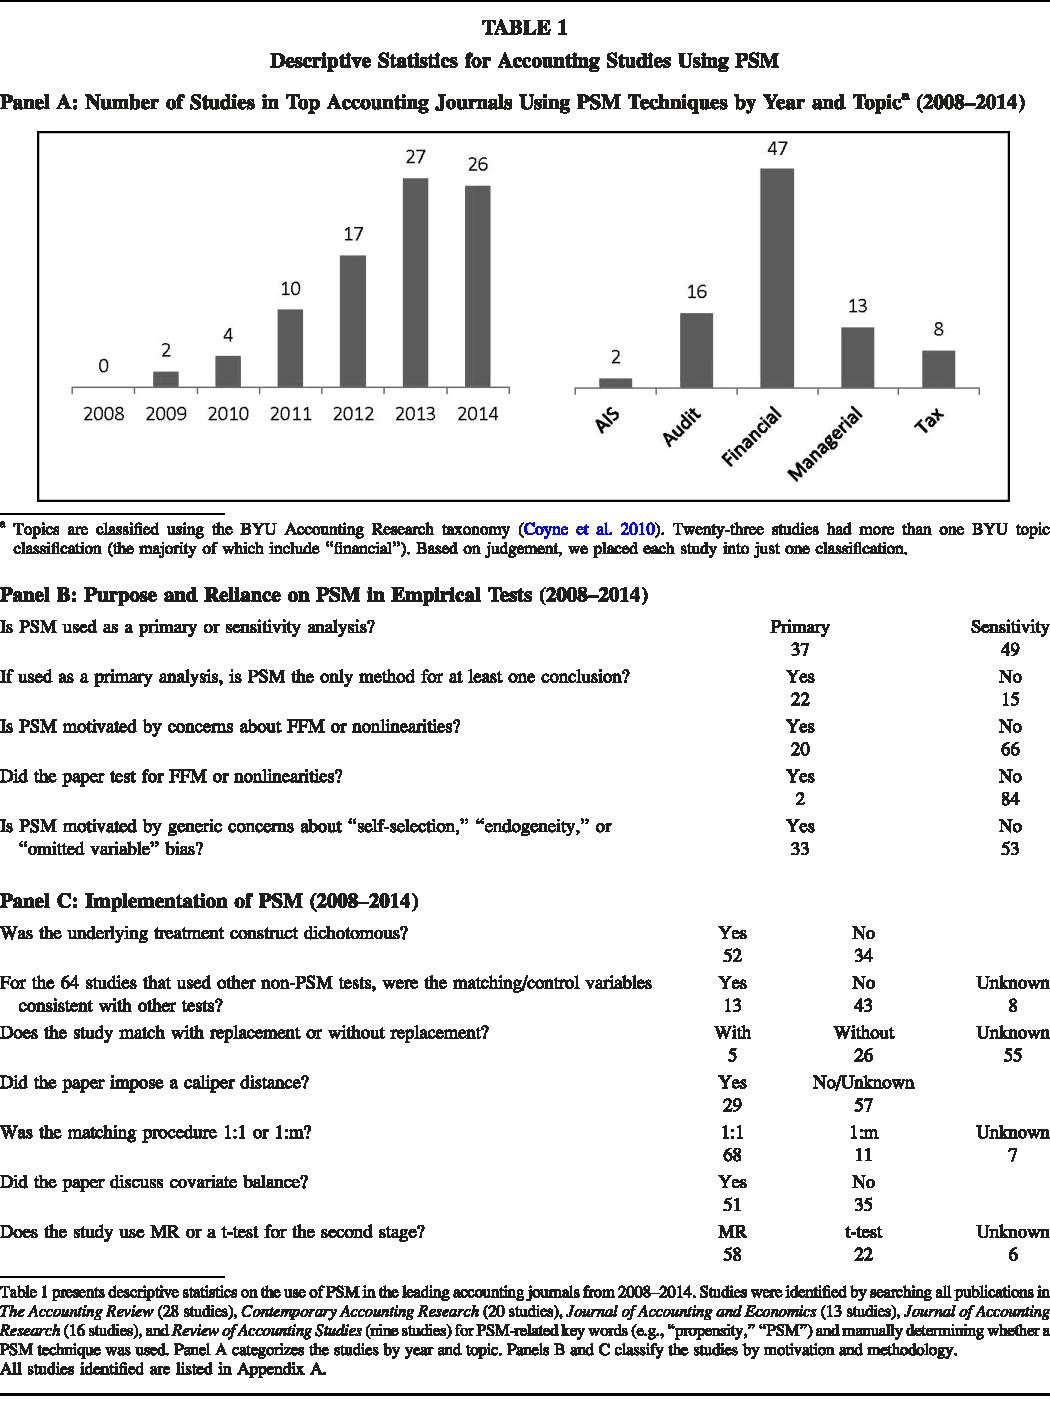
\includegraphics[width=16cm]{../table/tbl01.pdf}
\end{table}

\begin{itemize}
 \item 2008 $\sim$ 2014 年における、\textit{The Accounting Review,
       Contemporary Accounting Research, Journal of Accounting and
       Economics, Journal of Accounting Research, and Review of
       Accounting Studies} に掲載された論文延べ 86 件が対象。
 \item 会計研究で PSM が用いられはじめたのは最近 (86 件中 70 件は 2012
       $\sim$ 2014 の期間に刊行)。
\end{itemize}

\paragraph{各研究の PSM の位置付け (Table 1 Panel B)}

\begin{itemize}
 \item 主要な分析 (primary analyses) として用いている研究が 37 件である
       のに対し、ロバスト・チェック (sensitivity or robustness tests) と
       して用いている研究は 49 件。
 \item PSM を採用する理由として FFM や重回帰分析の線形性の仮定を挙げてい
       る研究はわずか 20 件。
 \item PSM が対処しうる内生性の問題を提示することなく、広く ``自己選択
       (self--selection),'' ``内生性 (endogeneity),'' および ``欠落変数
       バイアス (omitted variable bias)'' への対応として PSM を用いてい
       る研究が 33 件ある。
 \item Heckman (1979) の代わりとして誤用してしまっている研究も存在する。
\end{itemize}

\paragraph{処置群の選択の方法 (Table 1 Panel C)}

\begin{itemize}
 \item 問題の所在
       \begin{itemize}
        \item 処置が 2 値変数 (dichotomous) であるならば、PSM の実施は単純である。
        \item しかしながら、多様な状況でマッチングを実施するため、連続 (あるい
              は順序) 変数に閾値を設けて変換することがある\footnote{2 値
              変数を用いた処置群の選択について、例えば修正再表示のアナウ
              ンスメントや IFRS のアドプションがあげられる。一方で、非 2
              値変数を用いた処置群の選択について、企業の所有構造や監査人
              の産業特殊性 (auditor industry specialization) があげられ
              る}。
       \end{itemize}
 \item 問題点
       \begin{itemize}
        \item このような場合、閾値の近傍の観測値が over--represent される
              傾向があり、それによって、効果の大きさ (および平均処置効果)
              が消失し、第 II 種の過誤が生じる可能性が増大する。
       \end{itemize}
 \item 連続変数を用いている研究の数
       \begin{itemize}
        \item 34 件。また、この影響により、効果の大きさのみならずサンプ
              ル・サイズも低下する。
        \item 59 (12) 件の研究において、MR のサンプル・サイズの大きさは
              PSM の 3 (10) 倍である。
        \item サンプルサイズが小さいほど、サブサンプルは母集団を代表しな
              くなる。
       \end{itemize}
\end{itemize}

\paragraph{コントロール変数の選択 (Table 1 Panel C)}

\begin{itemize}
 \item MR と PSM のいずれを用いるにせよ、同様のコントロール変数を用いる
       べきであるにもかかわらず、しばしば異なるコントロール変数が用いら
       れていることがわかった。
 \item MR からマッチングに用いた変数を除外することは、その変数が処置変数
       (treatment) にも結果変数 (outcome) にも影響を与えないこと、
       ひいては、その変数によるマッチングが不必要であることを意味するに
       他ならない。
 \item 分析においては、\textit{post hoc} なモデルの特定 (model
       specification) をおこなっているという疑念 (appearance; 外観) を避
       けるため、PSM と他のテストとの説明変数の不一致を検討すべきである。
\end{itemize}

\paragraph{傾向スコア推定後のマッチング・プロシージャ (Table 1 Panel C)}

\begin{itemize}
 \item 置換処理 (replace)
       \begin{itemize}
        \item 55 件の研究において、マッチングに際して置換処理がおこなわ
              れているか否か (matching is performed with or without
              replacement) 開示されていない。
        \item 開示している 31 件の研究のうち、5 件が置換あり、26 件が置
              換なしであった。
       \end{itemize}
 \item キャリパー距離 (caliper distance)
       \begin{itemize}
        \item マッチング・プロシージャとしてキャリパー距離を開示して
              いる研究は 29 件のみ。
        \item 開示されているキャリパー距離の分布は、0.00005 から
              0.23 までで、よく用いられている距離は 0.01 (4 件)、0.03 (6
              件)、および 0.10 (5 件) である。
       \end{itemize}
 \item 1 対 1 と 1 対多のどちらのマッチングを用いるか
       \begin{itemize}
        \item 1 対 1 (one--to--one) が 68 instances であるのに対し、1 対
              多 (one--to--many) が 11 instances である。
       \end{itemize}
\end{itemize}

\paragraph{covariate balance (Table 1 Panel C)}

\begin{itemize}
 \item マッチング変数の数 (number of matching variables)、キャリパー距離
       (caliper distance)、グループ・サイズ (group size) などの要因は、
       PSM によってサンプルに covariate balance が生じる程度に影響する。
 \item しかしながら、covariate balance の決定はマッチング・クオリティ
       についての主観的な判断を要求するため、マッチングが実際に適切な
       (sufficient) balance を達成しているか否か、しばしば不透明である。
 \item サーベイの結果、35 件はマッチされたサンプル (matched sample) の
       covariate balance について議論しておらず、4 件のみ傾向スコ
       アの平均差について議論している。
 \item 研究においては、残存した covariate imbalance の効果を緩和するため
       に、PSM のサブサンプルにおいて MR を使うことができる。
 \item サーベイの結果、58 件は (第 2 段階の) ATE を推定する際に MR を用
       いている、22 件は結果変数の距離を t 検定することによって、処置効
       果を推定している、そして、6 件は推定手法を開示していないというこ
       とが明らかとなった。
\end{itemize}

\paragraph{サーベイの結論}

\begin{itemize}
 \item 本節で指摘した問題点は現在の文献でも改善されていない。
 \item Heckman (1979) モデルについて含意を示した Lennox et al. (2012,
       589) の結論と同様に、われわれは、多数の研究が ``重要な計量経済学
       上の問題点および PSM の利用をとりまく問題点に対する理解
       (appreciation) がほとんど無いままに、'' PSM を実施していると結論
       付ける。 
\end{itemize}
\section{EMPIRICAL EXAMPLES OF PROPENSITY SCORE MATICHNG IN ACCOUNTING SETTINGS}
監査法人の規模、内部統制、アナリストのフォロー数が財務報告の質に与える影響を検証する。

\subsection*{Sample Selection and Descriptive Statistics}

\paragraph{サンプルの選択}

\begin{itemize}
 \item 期間は、Sarbanes-Oxley (SOX) 法にかかる観測値が取得可能な2004〜2012年である。
 \item 以下の要件に該当するサンプルを除外する。
   \begin{itemize}
    \item 海外企業、および金融業(2桁SICコードの60--69)に属する観測値
    \item 総資産が500ドル以下の観測値
    \item 2桁SICコードに基づく産業年が10観測値未満のもの(裁量的会計発生高を計算するための要件)
    \item 欠損値のある観測値
   \end{itemize}
 \item 最終サンプルは、監査法人の規模の分析とアナリストのフォローの分析で29,227観測値、内部統制の弱さの分析で20,385観測値である。
 \item 最終サンプルの内訳は、以下のとおりである。
    \begin{itemize}
    \item Big 4に監査されている($\mathit{BIG}4_{it}=1$)のが19,988企業年
    \item 少なくとも1つの内部統制の弱さを監査報告書で指摘されている($\mathit{WEAK}_{it}=1$)のが1,422企業年
    \item 少なくとも1人のアナリストがついている($\mathit{ANALYST}_{it}=1$)21,144企業年
   \end{itemize}
\end{itemize}

\paragraph{データソース}

\begin{itemize}
 \item 監査法人、内部統制の弱さ、財務諸表の再報告にかかるデータ:Audit Analytics
 \item アナリストにかかるデータ:the Institutional Brokers’ Estimate System (I/B/E/S)
 \item 財務データ:Compustat
  \begin{itemize}
   \item Table 2:記述統計量
  \end{itemize}
\end{itemize}

\subsection*{Research Design}

$\mathit{BIG}4_{it}$、$\mathit{WEAK}_{it}$、$\mathit{ANALYST}_{it}$のそれぞれを割り当て変数とし、PSMを行い、ATEを推定する。

\paragraph{予測モデル(第1段階)}

\begin{equation}
\mathit{D}_{it} = \alpha_0 + \alpha_1 \mathit{X}_{it} + \varepsilon_{it}
\end{equation}

\begin{itemize}
 \item $\mathit{D}_{it}$は、$\mathit{BIG}4_{it}$、$\mathit{WEAK}_{it}$、$\mathit{ANALYST}_{it}$で、処置群と対照群に割り当てるダミー変数
 \item PSMのキャリパー距離は、0.03とする。
\end{itemize}

\paragraph{結果モデル(第2段階)}

\begin{equation}
\mathit{QUALITY}_{it} = \beta_0 + \beta_1 \mathit{D}_{it} + \beta_2 \mathit{X}_{it} +\varepsilon_{it}
\end{equation}

\begin{itemize}
 \item $\mathit{QUALITY}_{it}$は、財務報告の質を示し、本分析では、裁量的会計発生高($\mathit{ABSACC}_{it}$)、および財務諸表の再報告($\mathit{RESTATE}_{it}$)のそれぞれで評価している。
 \item $X_{it}$は、企業規模($\mathit{LNASSETS}_{it}$)、パフォーマンス($\mathit{ROA}_{it}$、$\mathit{ATURN}_{it}$)、財政状態($\mathit{CURR}_{it}$、$\mathit{LEV}_{it}$、$\mathit{DISTRESS}_{it}$)、設立年数($\mathit{AGE}_{it}$)、成長性($\mathit{GROWTH}_{it}$)、企業価値($\mathit{BTM}_{it}$)、年度固定効果を用いる。
  \begin{itemize}
   \item Appendix B:変数の定義
  \end{itemize}
 \item 本分析で観察したいATEは、(5)式の$\beta_1$で示される。
\end{itemize}

\subsection*{Diagnosing Function Form Misspecification}
\begin{itemize}
 \item MRにおいて、FFMが懸念されるのかについて判定する。
 \item Ramsey(1969)のRESETテストがFFMを見る手法として用いられることがある(Lawrence et al. 2011を見よ)。
 \item ただし、これは、変数の非線形性が追加的な説明を与えているのかどうかについて検証するものであり、結果変数と非線形な関係にある変数がATEの推定にバイアスを与えてるのかどうかを見るものではない。
\end{itemize}

\paragraph{変数を追加してFFMを判定する方法(Table 3)}

\begin{itemize}
 \item ここで、MRにおけるFFMを判定する手法として、コントロール変数(たとえば、変数を2乗したもの、3乗したもの)を追加する手法を提唱する。
 \item もし、元のモデルと変数を追加したモデルの結果が異なるのなら、FFMに対する懸念がある。
 \item (5)式を推定した結果を見ると、変数を追加したとしても((2)列と(5)列)、基本的な結果は元のモデル((1)列と(4)列)大きくは変わらない。
 \item しかし、監査法人の規模とアナリストのフォローで割り当てた場合、Chow(1960)の検定をすると、元のモデルのATEと変数を追加したモデルのATEの間で有意な差が認められる。
  \begin{itemize}
   \item これは、$X$と結果変数が非線形な関係にあることを示す。
  \end{itemize}
\end{itemize}

\subsection*{First-Stage Prediction Model}

\paragraph{第1段階((4)式)の推定結果(Table 4)}

\begin{itemize}
 \item 先行研究では、pseudo-${\rm R^2}$が高ければ高いほど、PSMは良い状態であることが示唆されている。
 \item しかし、この説明力は、割り当てが大きく影響を与えている。
 \item つまり、処置群の$X$が対照群の$X$とより大きく相違しているのなら、回帰式の説明力は大きくなる。
 \item overlapが大きければ大きいほど、pseudo-${\rm R^2}$は小さくなるとも言える。
  \begin{itemize}
   \item ただし、説明力がPSMの有効性を必ずしも示しているわけではない。
  \end{itemize}
\end{itemize}

\subsection*{Demonstration of Propensity Score Overlap}

処置群と対照群の傾向スコアのoverlapについて確認するため、Shaikh, Simonsen, Vydacil, and Yildiz(2009)と同様に、傾向スコアの密度をプロットする。

\paragraph{監査法人の規模で割り当てた場合の傾向スコアのプロット(Figure 1, Panel A)}

\begin{figure}
 \centering
 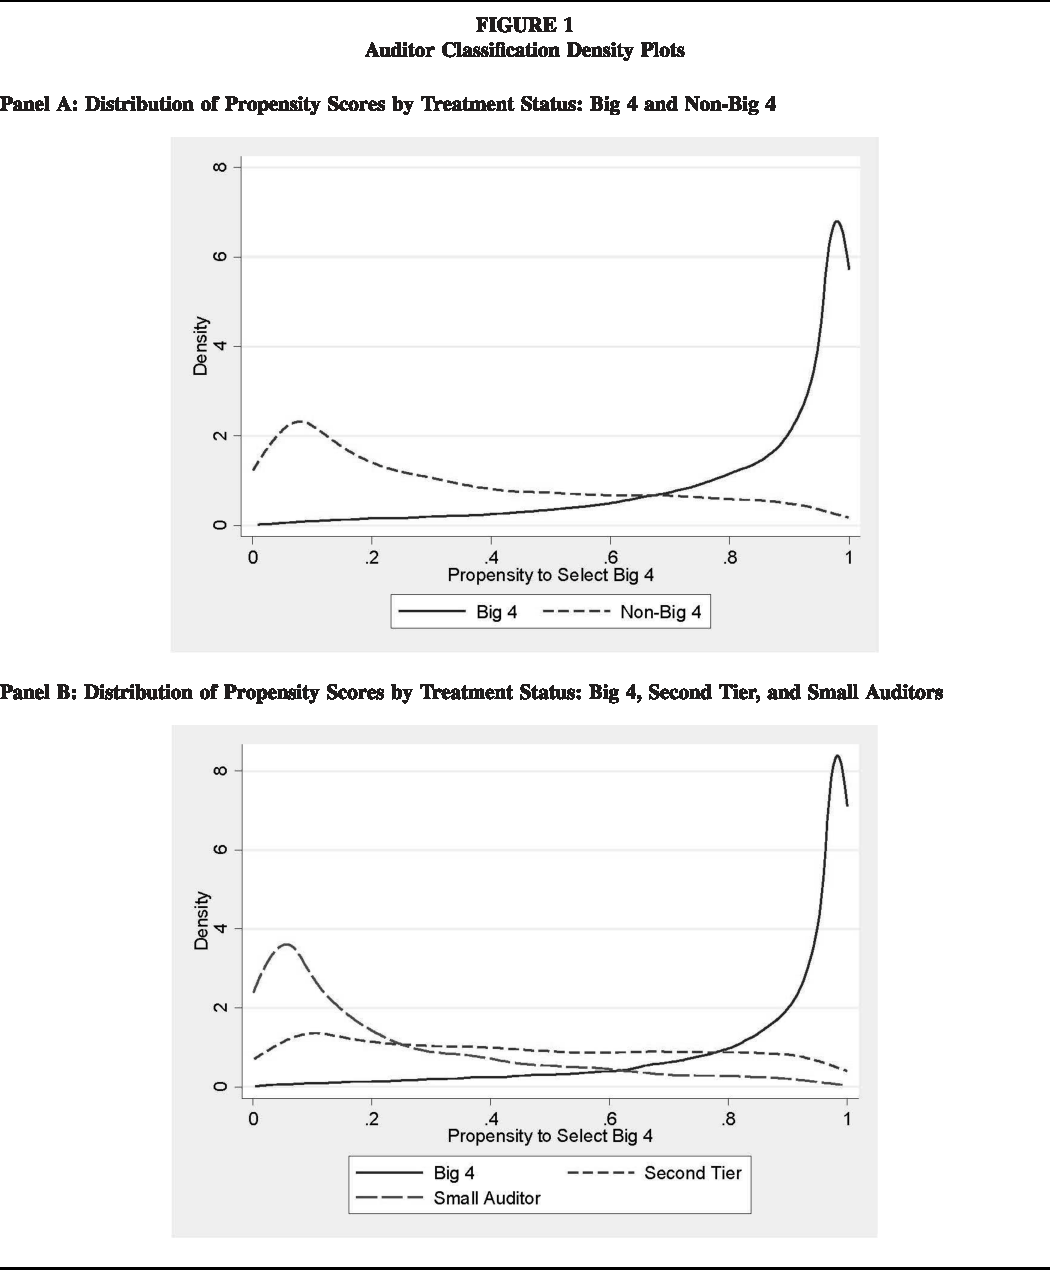
\includegraphics[width=16cm]{../fig/fig01.pdf}
\end{figure}

\begin{itemize}
 \item Big 4の監査法人のクライアントの傾向スコアは、0.9〜1の範囲内に集中し、非Big 4の監査法人のクライアントの傾向スコアは、0〜0.2に集中している。
 \item これは、共変量が割り当ての決定に大きく影響していることを示している。
 \item 結果的に、マッチングは、主として極端でない傾向スコアの範囲(ここでは、0.2〜0.9)の範囲内でなされることになる。
\end{itemize}

\paragraph{Second Tierを考慮して割り当てた場合の傾向スコアのプロット(Figure 1, Panel B)}

\begin{itemize}
 \item 非Big 4のクライアントから、Second Tierの監査法人のクライアントを識別する。
 \item この識別をしたプロットを見ると、Second Tierのクライアントは、0〜0.2の範囲内で、小規模監査法人のクライアントよりも傾向スコアが小さいが、0.2以上では小規模監査法人よりも大きな傾向スコアであることがわかる。
 \item これは、Second TierのクライアントがBig 4のクライアントとより多くマッチングが成立することを示す。
\end{itemize}

\paragraph{内部統制の弱さで割り当てた場合の傾向スコアの密度のプロット(Figure 2, Panel A)}

\begin{figure}
 \centering
 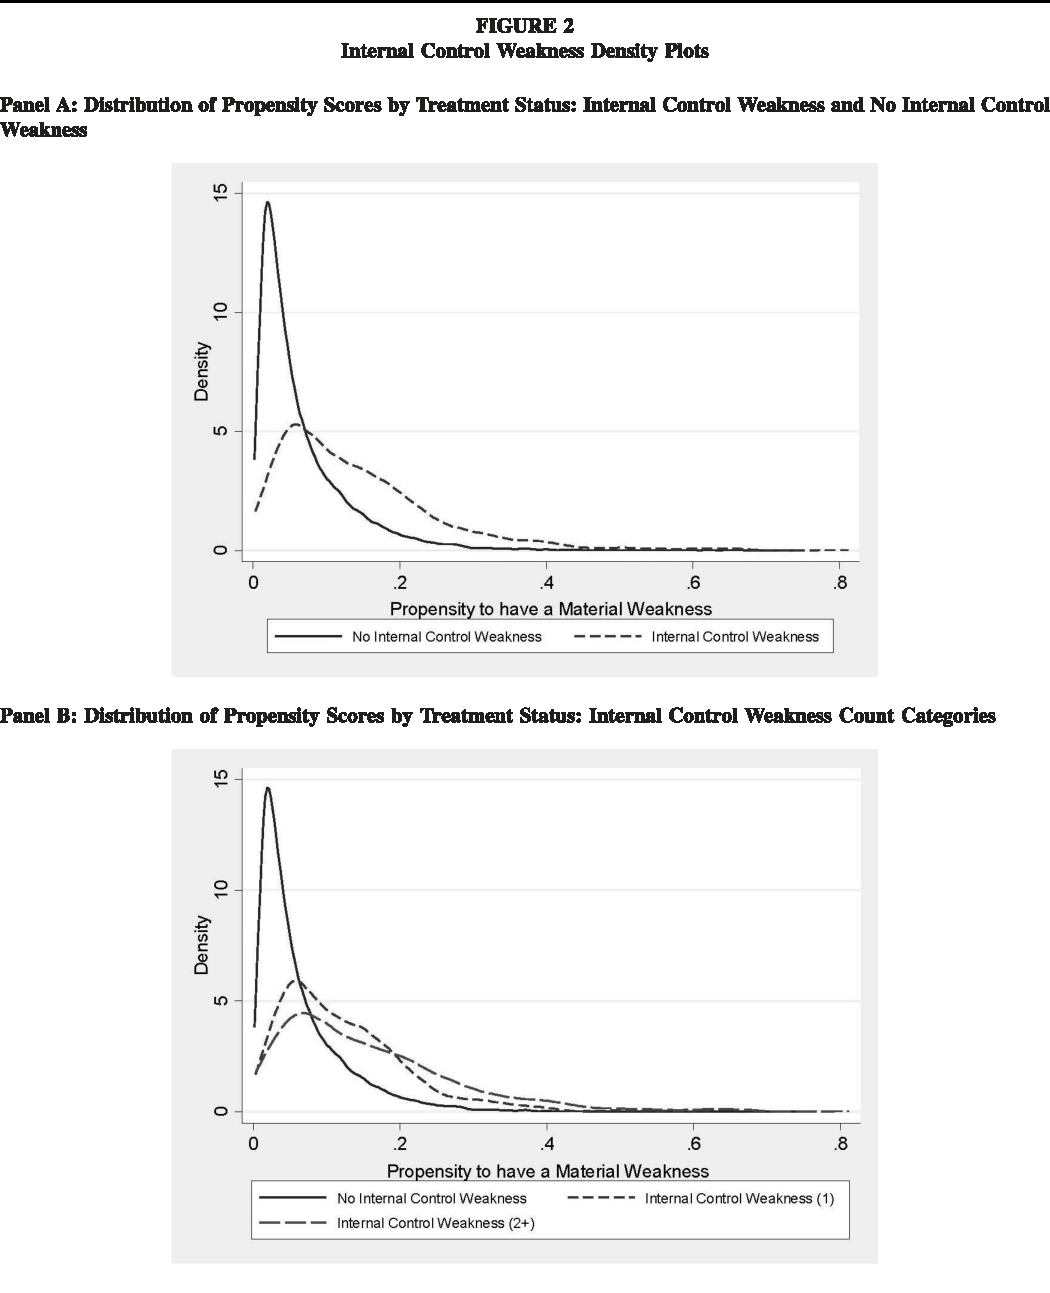
\includegraphics[width=16cm]{../fig/fig02.pdf}
\end{figure}

\begin{itemize}
 \item 監査法人の規模のときよりも、overlapの範囲が大きいことがわかる。
 \item Table 4のpseudo-${\rm R^2}$も、低い値であることもこのことを示唆している。
\end{itemize}

\paragraph{内部統制の弱さの判定を詳細にした場合の傾向スコアの密度のプロット(Figure 2, Panel B)}

\begin{itemize}
 \item 内部統制の弱さの判定をより詳細にする(No ICW、1 ICW、2+ICW)。
 \item 監査法人の規模の場合と同様に、overlapは、No ICWと2+ICWの間よりも、No ICWと1 ICWの間の方がより大きいことがわかる。
\end{itemize}

\paragraph{アナリストのフォローで割り当てた場合の傾向スコアの密度のプロット(Figure 3, Panel A)}

\begin{itemize}
 \item 監査法人の場合と同様に、処置群と対照群との間で傾向スコアの密度の範囲は異なっており、overlapが限定的なものであることがわかる。
\end{itemize}

\paragraph{アナリストのフォロー数を詳細にした場合の傾向スコアの密度のプロット(Figure 3, Panel B)}

\begin{itemize}
 \item アナリストのフォロー数を詳細にみる(1〜5人、6〜10人、11人以上)。
 \item プロットした結果、アナリストの数が少なければ少ないほど、アナリストに全くフォローされてない観測値とのoverlapが大きくなることがわかる。
 \item これは、マッチングがフォローしているアナリストの数の少ない企業となされる可能性が高いことを示している。
\end{itemize}

\subsection*{Matching without Replacement}

置き換えを認めず、1対1でマッチングを行う。

\paragraph{サンプルの構成(Table 5, Panel A)}

\begin{itemize}
 \item 置き換えをせず1対1でマッチングすると、かなりの数の観測値を除去することになる。
 \item 事実、“full sample”を比較して、監査法人の規模で30\%、内部統制の弱さで14\%、アナリストのフォローで28\%のサンプルしか確保できなかった。
 \item また、マッチングしたサンプルは、Second Tierのクライアントや、アナリストのフォロー数が少ない観測値で構成されていることもわかる。
  \begin{itemize}
   \item サンプルが小さいことは、外的な妥当性を減少させる、もしくは欠落させてしまう可能性を有している。
  \end{itemize}
\end{itemize}

\paragraph{MRとPSM間における共変量とATEの比較(Table 5, Panel B)}

\begin{itemize}
 \item 共変量は、PSMを行うことにより、バランスが向上していることがわかる。
  \begin{itemize}
   \item これは、MRにおいて、処置群と対照群の相違が残ったまま、ATEを推定していることを示す。
  \end{itemize}
 \item 裁量的会計発生高を従属変数とした場合、MRのATEはすべて有意であるが、PSMはすべて非有意であり、Chow(1960)の検定も、すべての係数間で有意である。
 \item 一方、財務諸表の再報告を従属変数とした場合は、MRとPSMのATEともにすべて類似した結果を示すが、係数を比較すると、有意な差が検出されるものが存在している。
\end{itemize}

\paragraph{まとめ}
\begin{itemize}
 \item 以上の分析から、MRとPSMでは推定される ATEが有意に異なっていることが明らかとなった。
 \item もし、PSMのみで分析すると、監査法人の規模、内部統制の弱さ、およびアナリストのフォローは、財務報告の質に影響を与えていないという結果のみを得ることになる。
 \item しかし、この ``帰無仮説を採択する'' (accept the null hypothesis) のは結論を急ぎ過ぎ (premature) であるかもしれない。
 \item 以下で、PSMの手法を変更することで、結果が変化することを示す。
\end{itemize}

\subsection*{Matching with Replacement}

置き換えを認めて、1対1でマッチングを行う。

\paragraph{サンプルの構成(Table 6, Panel B)}

\begin{itemize}
 \item (2)列目は、サンプルサイズが小さい方の群を処置群とし、サンプルサイズの大きな方の群にマッチングの置き換えを認める場合の結果である(Panel A)。
 \item サンプルサイズが大きくなっており、キャリパー距離(0.03)の間でより多くの対照群の観測値がマッチングしていることがわかる。
 \item (3)列目は、サンプルサイズの大きな方の群を処置群とし、サンプルサイズの小さい方の群にマッチングの置き換えを認める場合の結果である。
 \item サンプルサイズがかなり大きくなっており、ウェイトがいずれも5以上であることから、対照群の観測値がより多くの回数マッチングしていることがわかる。
 \item マッチングの手法ごとにサンプルの構成を比較した結果、9個の比較中8個で有意な差が認められる。
 \item 特に、Second Tierのクライアントの割合と、アナリストのフォロー数の平均値は、マッチングの手法間で顕著な差がある。
  \begin{itemize}
   \item マッチング手法の違いが、サンプルサイズとサンプルの構成に影響を与えてしまうことが示唆されている。
  \end{itemize}
\end{itemize}

\paragraph{ATEの比較(Table 6, Panel B, C)}

\begin{itemize}
 \item 監査法人の規模で割り当てた場合の結果は、いずれも非有意である。
 \item しかし、ATEの差が有意に検出されているものが存在する(6個の比較中3個)。
 \item 内部統制の弱さ、およびアナリストのフォローで割り当てた場合の結果は、マッチングの手法ごとに異なっており、ATEの差も有意に検出されているものがある(12個の比較中7個)。
  \begin{itemize}
   \item マッチングの手法が統計的な結果に影響を与えてしまう。
  \end{itemize}
\end{itemize}

\subsection*{The Influence of Matching Variables on Estimates of the ATE}

\paragraph{変数を置き換えてマッチングを行なった場合のサンプルの構成(Table 7, Panel A)}

\begin{itemize}
 \item 企業規模を示す変数を、総資産の自然対数($\mathit{LNASSETS}_{it}$)から時価総額の自然対数($\mathit{LNMARKET}_{it}$)に入れ替える。
 \item マッチングの手法間でサンプルを比較すると、共通の観測値は、58.9〜71.4\%の割合である。
 \item さらに、内部統制の弱さで割り当てた場合の対照群(内部統制の弱さが指摘されていない観測値)は、マッチングの手法間で、わずか18.2\%しかサンプルが共通してない。
\end{itemize}

\paragraph{変数を置き換えてマッチングを行なった場合のATE(Table 7, Panel B)}

\begin{itemize}
 \item $\mathit{LNASSETS}_{it}$のATEよりも、$\mathit{LNMARKET}_{it}$のATEの方が、有意であるものが多いことがわかる。
 \item 特に、アナリストのフォローで割り当てとし、財務諸表の再報告を従属変数とした時のATEは、Table 5の全サンプルとマッチングサンプルで非有意だったにもかかわらず、変数を置き換えると有意な結果が確認される。
 \item Chow(1960)の検定によれば、6個の比較中、3個でATEが有意な差であることが確認される。
\end{itemize}

\paragraph{変数を追加してマッチングを行った場合の結果(Table 8)}

\begin{itemize}
 \item 以下のとおり、変数を追加してマッチングを行う。
  \begin{itemize}
   \item 監査法人の規模:営業活動にかかるキャッシュフロー($\mathit{CFO}_{it}$)、海外売上高($\mathit{FOREIGN}_{it}$)
   \item 内部統制の弱さ:損失ダミー($\mathit{LOSS}_{it}$)
   \item アナリストのフォロー:$\mathit{LNMARKET}_{it}$
  \end{itemize}
 \item このマッチングからATEを求めた結果は、(2)列目と(5)列目に示されているが、いずれも有意であることがわかる。
 \item さらに以下のとおり変数を追加する。
  \begin{itemize}
   \item 監査法人の規模:$\mathit{LNASSETS}_{it-1}$、$LOSS_{it}$、棚卸資産($\mathit{INVENTORY}_{it}$)
   \item 内部統制の弱さ:$\mathit{FOREIGN}_{it}$
   \item アナリストのフォロー:$\mathit{BTM}_{it-1}$
  \end{itemize}
 \item 以上でマッチングし、ATEを求めた結果は、(3)列目と(6)列目に示されているが、これまでの検証で一貫して有意である内部統制の弱さで割り当て、財務諸表の再報告を従属変数としたATE以外、すべて非有意である。
  \begin{itemize}
   \item 以上から、ATEの推定は、PSMのモデルの設定から影響を受けやすいことが明らかである。
  \end{itemize}
 \item 以上の変数の選択は、結果の頑健性を示すために、``事後的''に選択されたことに留意するべきである。
 \item すべての$X$は、結果に同じような影響を与えるとは限らない。
  \begin{itemize}
   \item ここから、PSMの変数の選択において、十分な考慮をするこの重要さが示唆される。
  \end{itemize}
\end{itemize}

\section{EMPIRICAL EXAMPLES OF PROPENSITY SCORE MATICHNG IN ACCOUNTING SETTINGS}
監査法人の規模、内部統制、アナリストのフォロー数が財務報告の質に与える影響を検証する。

\subsection*{Sample Selection and Descriptive Statistics}

\paragraph{サンプルの選択}

\begin{itemize}
 \item 期間は、Sarbanes-Oxley (SOX) 法にかかる観測値が取得可能な2004〜2012年である。
 \item 以下の要件に該当するサンプルを除外する。
   \begin{itemize}
    \item 海外企業、および金融業(2桁SICコードの60--69)に属する観測値
    \item 総資産が500ドル以下の観測値
    \item 2桁SICコードに基づく産業年が10観測値未満のもの(裁量的会計発生高を計算するための要件)
    \item 欠損値のある観測値
   \end{itemize}
 \item 最終サンプルは、監査法人の規模の分析とアナリストのフォローの分析で29,227観測値、内部統制の弱さの分析で20,385観測値である。
 \item 最終サンプルの内訳は、以下のとおりである。
    \begin{itemize}
    \item Big 4に監査されている($\mathit{BIG}4_{it}=1$)のが19,988企業年
    \item 少なくとも1つの内部統制の弱さを監査報告書で指摘されている($\mathit{WEAK}_{it}=1$)のが1,422企業年
    \item 少なくとも1人のアナリストがついている($\mathit{ANALYST}_{it}=1$)21,144企業年
   \end{itemize}
\end{itemize}

\paragraph{データソース}

\begin{itemize}
 \item 監査法人、内部統制の弱さ、財務諸表の再報告にかかるデータ:Audit Analytics
 \item アナリストにかかるデータ:the Institutional Brokers’ Estimate System (I/B/E/S)
 \item 財務データ:Compustat
  \begin{itemize}
   \item Table 2:記述統計量
  \end{itemize}
\end{itemize}

\subsection*{Research Design}

$\mathit{BIG}4_{it}$、$\mathit{WEAK}_{it}$、$\mathit{ANALYST}_{it}$のそれぞれを割り当て変数とし、PSMを行い、ATEを推定する。

\paragraph{予測モデル(第1段階)}

\begin{equation}
\mathit{D}_{it} = \alpha_0 + \alpha_1 \mathit{X}_{it} + \varepsilon_{it}
\end{equation}

\begin{itemize}
 \item $\mathit{D}_{it}$は、$\mathit{BIG}4_{it}$、$\mathit{WEAK}_{it}$、$\mathit{ANALYST}_{it}$で、処置群と対照群に割り当てるダミー変数
 \item PSMのキャリパー距離は、0.03とする。
\end{itemize}

\paragraph{結果モデル(第2段階)}

\begin{equation}
\mathit{QUALITY}_{it} = \beta_0 + \beta_1 \mathit{D}_{it} + \beta_2 \mathit{X}_{it} +\varepsilon_{it}
\end{equation}

\begin{itemize}
 \item $\mathit{QUALITY}_{it}$は、財務報告の質を示し、本分析では、裁量的会計発生高($\mathit{ABSACC}_{it}$)、および財務諸表の再報告($\mathit{RESTATE}_{it}$)のそれぞれで評価している。
 \item $X_{it}$は、企業規模($\mathit{LNASSETS}_{it}$)、パフォーマンス($\mathit{ROA}_{it}$、$\mathit{ATURN}_{it}$)、財政状態($\mathit{CURR}_{it}$、$\mathit{LEV}_{it}$、$\mathit{DISTRESS}_{it}$)、設立年数($\mathit{AGE}_{it}$)、成長性($\mathit{GROWTH}_{it}$)、企業価値($\mathit{BTM}_{it}$)、年度固定効果を用いる。
  \begin{itemize}
   \item Appendix B:変数の定義
  \end{itemize}
 \item 本分析で観察したいATEは、(5)式の$\beta_1$で示される。
\end{itemize}

\subsection*{Diagnosing Function Form Misspecification}
\begin{itemize}
 \item MRにおいて、FFMが懸念されるのかについて判定する。
 \item Ramsey(1969)のRESETテストがFFMを見る手法として用いられることがある(Lawrence et al. 2011を見よ)。
 \item ただし、これは、変数の非線形性が追加的な説明を与えているのかどうかについて検証するものであり、結果変数と非線形な関係にある変数がATEの推定にバイアスを与えてるのかどうかを見るものではない。
\end{itemize}

\paragraph{変数を追加してFFMを判定する方法(Table 3)}

\begin{itemize}
 \item ここで、MRにおけるFFMを判定する手法として、コントロール変数(たとえば、変数を2乗したもの、3乗したもの)を追加する手法を提唱する。
 \item もし、元のモデルと変数を追加したモデルの結果が異なるのなら、FFMに対する懸念がある。
 \item (5)式を推定した結果を見ると、変数を追加したとしても((2)列と(5)列)、基本的な結果は元のモデル((1)列と(4)列)大きくは変わらない。
 \item しかし、監査法人の規模とアナリストのフォローで割り当てた場合、Chow(1960)の検定をすると、元のモデルのATEと変数を追加したモデルのATEの間で有意な差が認められる。
  \begin{itemize}
   \item これは、$X$と結果変数が非線形な関係にあることを示す。
  \end{itemize}
\end{itemize}

\subsection*{First-Stage Prediction Model}

\paragraph{第1段階((4)式)の推定結果(Table 4)}

\begin{itemize}
 \item 先行研究では、pseudo-${\rm R^2}$が高ければ高いほど、PSMは良い状態であることが示唆されている。
 \item しかし、この説明力は、割り当てが大きく影響を与えている。
 \item つまり、処置群の$X$が対照群の$X$とより大きく相違しているのなら、回帰式の説明力は大きくなる。
 \item overlapが大きければ大きいほど、pseudo-${\rm R^2}$は小さくなるとも言える。
  \begin{itemize}
   \item ただし、説明力がPSMの有効性を必ずしも示しているわけではない。
  \end{itemize}
\end{itemize}

\subsection*{Demonstration of Propensity Score Overlap}

処置群と対照群の傾向スコアのoverlapについて確認するため、Shaikh, Simonsen, Vydacil, and Yildiz(2009)と同様に、傾向スコアの密度をプロットする。

\paragraph{監査法人の規模で割り当てた場合の傾向スコアのプロット(Figure 1, Panel A)}

\begin{figure}
 \centering
 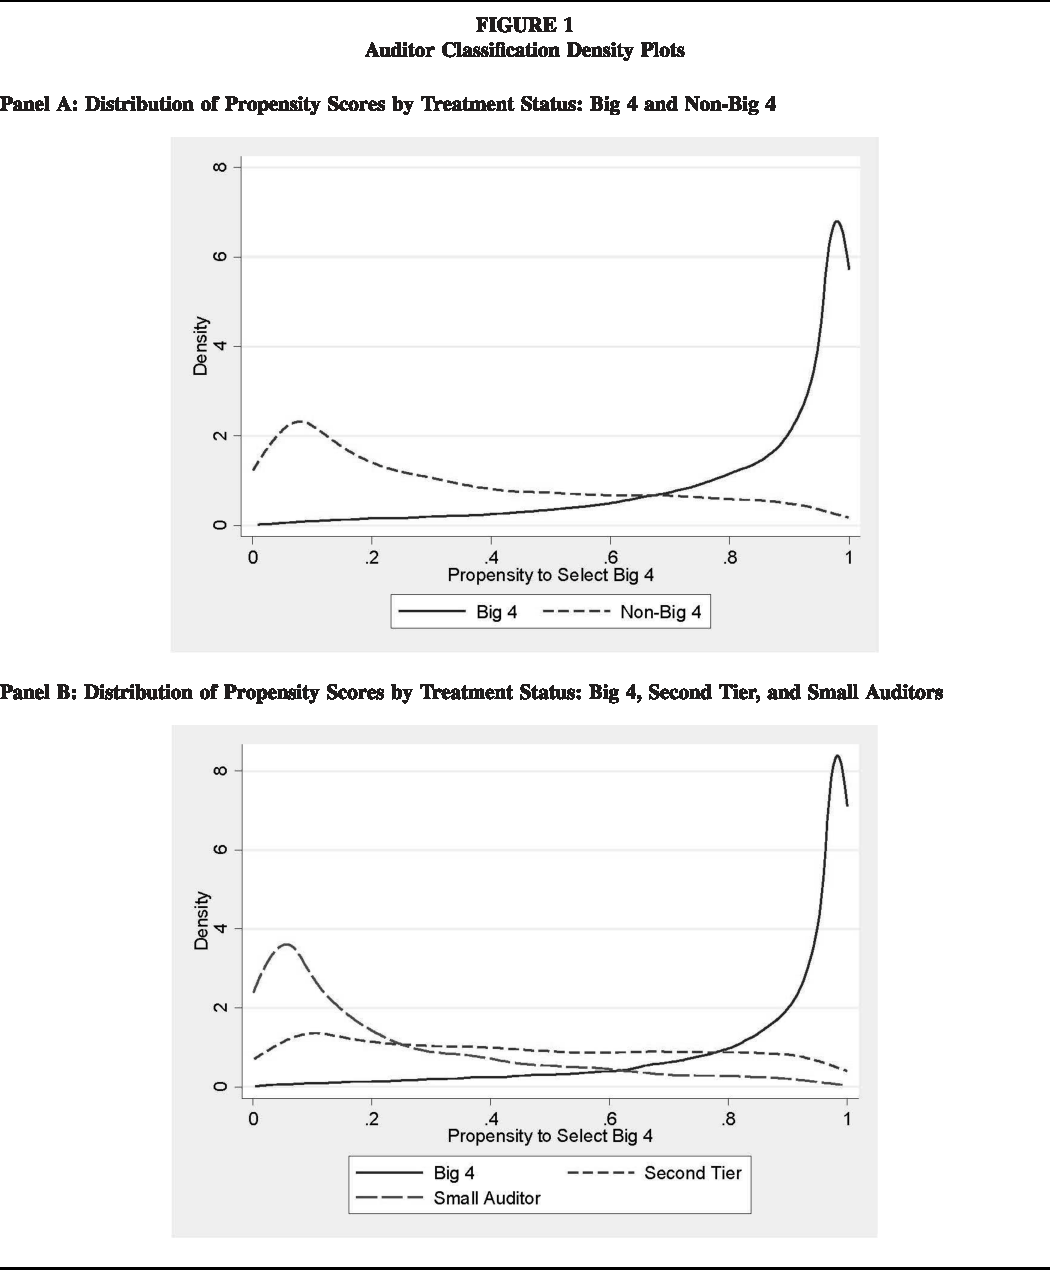
\includegraphics[width=16cm]{../fig/fig01.pdf}
\end{figure}

\begin{itemize}
 \item Big 4の監査法人のクライアントの傾向スコアは、0.9〜1の範囲内に集中し、非Big 4の監査法人のクライアントの傾向スコアは、0〜0.2に集中している。
 \item これは、共変量が割り当ての決定に大きく影響していることを示している。
 \item 結果的に、マッチングは、主として極端でない傾向スコアの範囲(ここでは、0.2〜0.9)の範囲内でなされることになる。
\end{itemize}

\paragraph{Second Tierを考慮して割り当てた場合の傾向スコアのプロット(Figure 1, Panel B)}

\begin{itemize}
 \item 非Big 4のクライアントから、Second Tierの監査法人のクライアントを識別する。
 \item この識別をしたプロットを見ると、Second Tierのクライアントは、0〜0.2の範囲内で、小規模監査法人のクライアントよりも傾向スコアが小さいが、0.2以上では小規模監査法人よりも大きな傾向スコアであることがわかる。
 \item これは、Second TierのクライアントがBig 4のクライアントとより多くマッチングが成立することを示す。
\end{itemize}

\paragraph{内部統制の弱さで割り当てた場合の傾向スコアの密度のプロット(Figure 2, Panel A)}

\begin{figure}
 \centering
 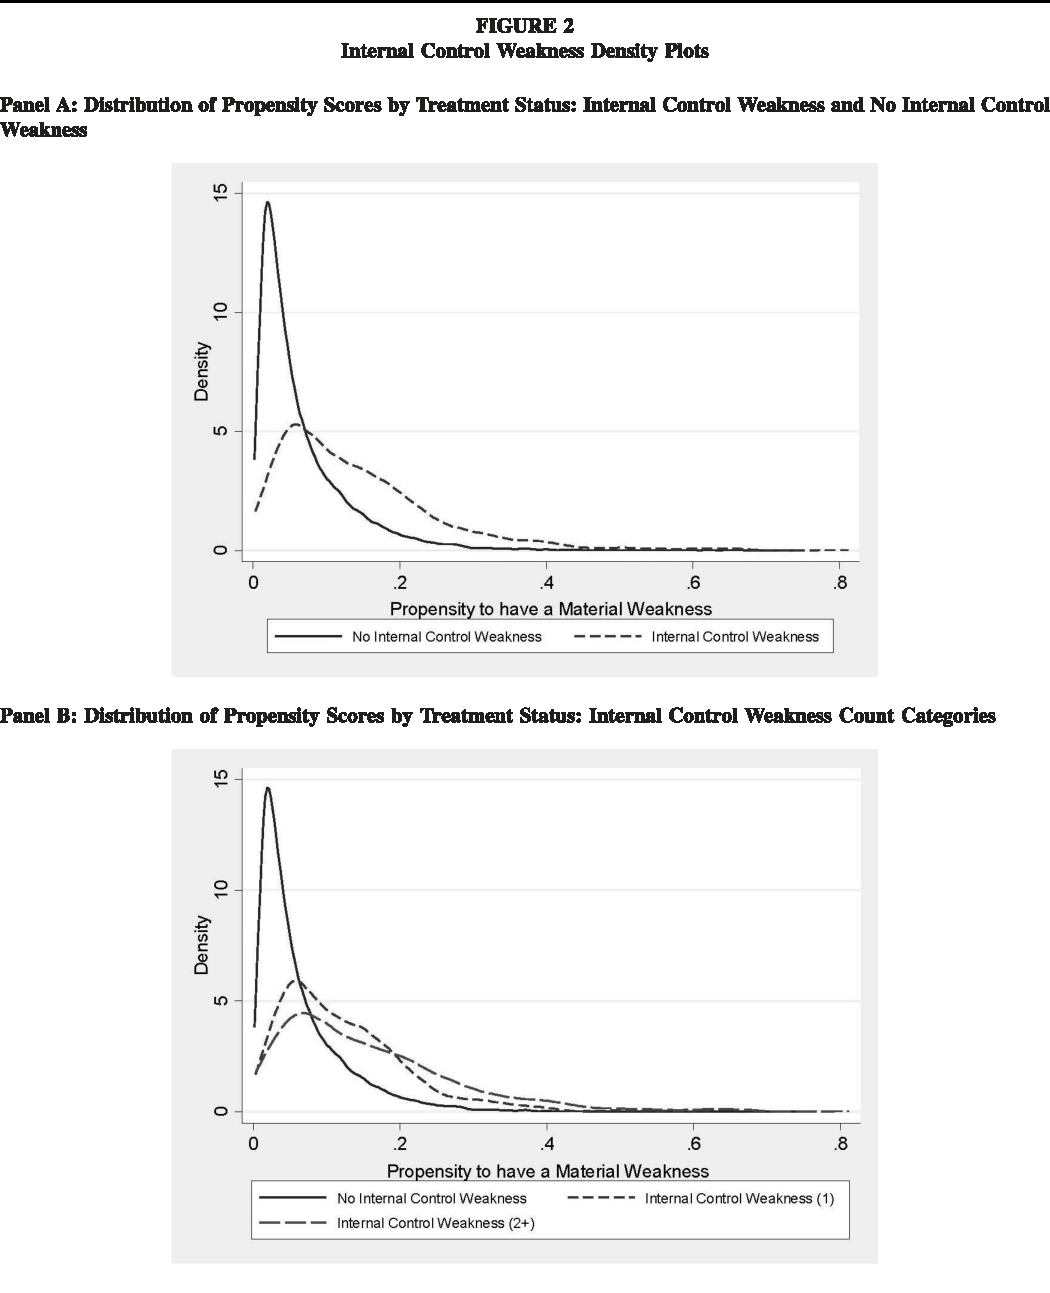
\includegraphics[width=16cm]{../fig/fig02.pdf}
\end{figure}

\begin{itemize}
 \item 監査法人の規模のときよりも、overlapの範囲が大きいことがわかる。
 \item Table 4のpseudo-${\rm R^2}$も、低い値であることもこのことを示唆している。
\end{itemize}

\paragraph{内部統制の弱さの判定を詳細にした場合の傾向スコアの密度のプロット(Figure 2, Panel B)}

\begin{itemize}
 \item 内部統制の弱さの判定をより詳細にする(No ICW、1 ICW、2+ICW)。
 \item 監査法人の規模の場合と同様に、overlapは、No ICWと2+ICWの間よりも、No ICWと1 ICWの間の方がより大きいことがわかる。
\end{itemize}

\paragraph{アナリストのフォローで割り当てた場合の傾向スコアの密度のプロット(Figure 3, Panel A)}

\begin{itemize}
 \item 監査法人の場合と同様に、処置群と対照群との間で傾向スコアの密度の範囲は異なっており、overlapが限定的なものであることがわかる。
\end{itemize}

\paragraph{アナリストのフォロー数を詳細にした場合の傾向スコアの密度のプロット(Figure 3, Panel B)}

\begin{itemize}
 \item アナリストのフォロー数を詳細にみる(1〜5人、6〜10人、11人以上)。
 \item プロットした結果、アナリストの数が少なければ少ないほど、アナリストに全くフォローされてない観測値とのoverlapが大きくなることがわかる。
 \item これは、マッチングがフォローしているアナリストの数の少ない企業となされる可能性が高いことを示している。
\end{itemize}

\subsection*{Matching without Replacement}

置き換えを認めず、1対1でマッチングを行う。

\paragraph{サンプルの構成(Table 5, Panel A)}

\begin{itemize}
 \item 置き換えをせず1対1でマッチングすると、かなりの数の観測値を除去することになる。
 \item 事実、“full sample”を比較して、監査法人の規模で30\%、内部統制の弱さで14\%、アナリストのフォローで28\%のサンプルしか確保できなかった。
 \item また、マッチングしたサンプルは、Second Tierのクライアントや、アナリストのフォロー数が少ない観測値で構成されていることもわかる。
  \begin{itemize}
   \item サンプルが小さいことは、外的な妥当性を減少させる、もしくは欠落させてしまう可能性を有している。
  \end{itemize}
\end{itemize}

\paragraph{MRとPSM間における共変量とATEの比較(Table 5, Panel B)}

\begin{itemize}
 \item 共変量は、PSMを行うことにより、バランスが向上していることがわかる。
  \begin{itemize}
   \item これは、MRにおいて、処置群と対照群の相違が残ったまま、ATEを推定していることを示す。
  \end{itemize}
 \item 裁量的会計発生高を従属変数とした場合、MRのATEはすべて有意であるが、PSMはすべて非有意であり、Chow(1960)の検定も、すべての係数間で有意である。
 \item 一方、財務諸表の再報告を従属変数とした場合は、MRとPSMのATEともにすべて類似した結果を示すが、係数を比較すると、有意な差が検出されるものが存在している。
\end{itemize}

\paragraph{まとめ}
\begin{itemize}
 \item 以上の分析から、MRとPSMでは推定される ATEが有意に異なっていることが明らかとなった。
 \item もし、PSMのみで分析すると、監査法人の規模、内部統制の弱さ、およびアナリストのフォローは、財務報告の質に影響を与えていないという結果のみを得ることになる。
 \item しかし、この ``帰無仮説を採択する'' (accept the null hypothesis) のは結論を急ぎ過ぎ (premature) であるかもしれない。
 \item 以下で、PSMの手法を変更することで、結果が変化することを示す。
\end{itemize}

\subsection*{Matching with Replacement}

置き換えを認めて、1対1でマッチングを行う。

\paragraph{サンプルの構成(Table 6, Panel B)}

\begin{itemize}
 \item (2)列目は、サンプルサイズが小さい方の群を処置群とし、サンプルサイズの大きな方の群にマッチングの置き換えを認める場合の結果である(Panel A)。
 \item サンプルサイズが大きくなっており、キャリパー距離(0.03)の間でより多くの対照群の観測値がマッチングしていることがわかる。
 \item (3)列目は、サンプルサイズの大きな方の群を処置群とし、サンプルサイズの小さい方の群にマッチングの置き換えを認める場合の結果である。
 \item サンプルサイズがかなり大きくなっており、ウェイトがいずれも5以上であることから、対照群の観測値がより多くの回数マッチングしていることがわかる。
 \item マッチングの手法ごとにサンプルの構成を比較した結果、9個の比較中8個で有意な差が認められる。
 \item 特に、Second Tierのクライアントの割合と、アナリストのフォロー数の平均値は、マッチングの手法間で顕著な差がある。
  \begin{itemize}
   \item マッチング手法の違いが、サンプルサイズとサンプルの構成に影響を与えてしまうことが示唆されている。
  \end{itemize}
\end{itemize}

\paragraph{ATEの比較(Table 6, Panel B, C)}

\begin{itemize}
 \item 監査法人の規模で割り当てた場合の結果は、いずれも非有意である。
 \item しかし、ATEの差が有意に検出されているものが存在する(6個の比較中3個)。
 \item 内部統制の弱さ、およびアナリストのフォローで割り当てた場合の結果は、マッチングの手法ごとに異なっており、ATEの差も有意に検出されているものがある(12個の比較中7個)。
  \begin{itemize}
   \item マッチングの手法が統計的な結果に影響を与えてしまう。
  \end{itemize}
\end{itemize}

\subsection*{The Influence of Matching Variables on Estimates of the ATE}

\paragraph{変数を置き換えてマッチングを行なった場合のサンプルの構成(Table 7, Panel A)}

\begin{itemize}
 \item 企業規模を示す変数を、総資産の自然対数($\mathit{LNASSETS}_{it}$)から時価総額の自然対数($\mathit{LNMARKET}_{it}$)に入れ替える。
 \item マッチングの手法間でサンプルを比較すると、共通の観測値は、58.9〜71.4\%の割合である。
 \item さらに、内部統制の弱さで割り当てた場合の対照群(内部統制の弱さが指摘されていない観測値)は、マッチングの手法間で、わずか18.2\%しかサンプルが共通してない。
\end{itemize}

\paragraph{変数を置き換えてマッチングを行なった場合のATE(Table 7, Panel B)}

\begin{itemize}
 \item $\mathit{LNASSETS}_{it}$のATEよりも、$\mathit{LNMARKET}_{it}$のATEの方が、有意であるものが多いことがわかる。
 \item 特に、アナリストのフォローで割り当てとし、財務諸表の再報告を従属変数とした時のATEは、Table 5の全サンプルとマッチングサンプルで非有意だったにもかかわらず、変数を置き換えると有意な結果が確認される。
 \item Chow(1960)の検定によれば、6個の比較中、3個でATEが有意な差であることが確認される。
\end{itemize}

\paragraph{変数を追加してマッチングを行った場合の結果(Table 8)}

\begin{itemize}
 \item 以下のとおり、変数を追加してマッチングを行う。
  \begin{itemize}
   \item 監査法人の規模:営業活動にかかるキャッシュフロー($\mathit{CFO}_{it}$)、海外売上高($\mathit{FOREIGN}_{it}$)
   \item 内部統制の弱さ:損失ダミー($\mathit{LOSS}_{it}$)
   \item アナリストのフォロー:$\mathit{LNMARKET}_{it}$
  \end{itemize}
 \item このマッチングからATEを求めた結果は、(2)列目と(5)列目に示されているが、いずれも有意であることがわかる。
 \item さらに以下のとおり変数を追加する。
  \begin{itemize}
   \item 監査法人の規模:$\mathit{LNASSETS}_{it-1}$、$LOSS_{it}$、棚卸資産($\mathit{INVENTORY}_{it}$)
   \item 内部統制の弱さ:$\mathit{FOREIGN}_{it}$
   \item アナリストのフォロー:$\mathit{BTM}_{it-1}$
  \end{itemize}
 \item 以上でマッチングし、ATEを求めた結果は、(3)列目と(6)列目に示されているが、これまでの検証で一貫して有意である内部統制の弱さで割り当て、財務諸表の再報告を従属変数としたATE以外、すべて非有意である。
  \begin{itemize}
   \item 以上から、ATEの推定は、PSMのモデルの設定から影響を受けやすいことが明らかである。
  \end{itemize}
 \item 以上の変数の選択は、結果の頑健性を示すために、``事後的''に選択されたことに留意するべきである。
 \item すべての$X$は、結果に同じような影響を与えるとは限らない。
  \begin{itemize}
   \item ここから、PSMの変数の選択において、十分な考慮をするこの重要さが示唆される。
  \end{itemize}
\end{itemize}

\section{Suggestions and consideration for future research}
\paragraph{本節の検討内容}
\begin{itemize}
 \item 内生性問題に対する``特効薬''は存在しないため、
       あらゆる方法で慎重に検討する必要がある。
 \item PSMは、観測不可能な要因を選択する上での内生性を特定するものではないが、
       FFMに関する内生性については、有用であると考えられる。
 \item 本節では、PSMを利用する上でより説得力を高めるための提言と、
       PSMを利用した分析結果を評価する際に検討すべき事項について述べる。
\end{itemize}

\subsection{Suggestions for improved application of propensity score matching}
\paragraph{PSMの利用を検討している研究に対する提言}
\begin{enumerate}
 \item FFMに関する識別問題に取り組むための手段としてPSMを利用すべきあり、PSMが
       ``内生性''``自己選択''``欠落変数バイアス''に関する一般的な懸念事項を緩和すると
       示唆するのは避けるべきである。
 \item PSMを利用した単一の (もしくは小数の) の結果だけをもとに、推論を行うべきではない。
       \begin{itemize}
        \item ``マッチング手法は回帰の修正 (regression adjustment) と
              対立するものではないと認識されるべきであり、実際、その2つの手法は補完的であり、
              組み合わせて使用することが望ましい。'' (Stuart, 2010, 2)
       \end{itemize}
 \item PSMとMRの両方を利用する場合、
       PSMのマッチング段階において、MRから除かれる変数を含めるべきではない。
       \begin{itemize}
        \item MRで除かれる変数についてマッチングを行うことで、
              MRとPSMが不均一 (unequal) になり、一方もしくは両者の特性 (specifications) に
              疑問が生じることになる。
        \item PSMの第2段階において、
              全てのコントロール変数を含めてMRを推定した場合の処置効果を推定すべき (``二重にロバストな推定'' (``doubly robust''estimation))
       \end{itemize}
 \item リサーチ・デザインの再現可能性と明瞭性を高めるために、
       PSMの設定を開示すべきである。具体的な内容は以下の通りである。
       \begin{enumerate}
        \item 傾向スコアを推定するためのモデル (第1段階)
        \item ATEを推定するためのモデル (第2段階)
        \item マッチング手法によって観測値を置き替えるか否か
        \item 処置済みの各観測値 (treated observation) に対して、マッチさせたコントロールの観測値数
        \item (実施する場合、) キャリパー距離 (caliper distance)
        \item マッチングの質 (共変量のバランス (covariate balance))
       \end{enumerate}
\end{enumerate}

\subsection{Considerations when using propensity score matching}
\paragraph{PSMを利用している場合の検討事項}
\begin{enumerate}
 \item 処置特性 (treatment specification) に関する検討
       \begin{itemize}
        \item 適切なマッチングの数が十分に存在している場合、
              効果量が最大となるような、母集団から抽出した部分集合に焦点をあてるために、
              ``最大限の''処置を施された観測値を``最小限の''処置を施された観測値に
              マッチさせることを、代替的手法として推奨する。
       \end{itemize}
 \item マッチング変数と処置効果の関係に関する検討
       \begin{itemize}
        \item treatmentの選択を決定する性質も、因果効果 (the effect of treatment) に関連している
              可能性がある。
        \item 機械的に、``最大の''因果効果を持つ観測値を選択し、また、``最小の''効果を維持させることで、
              PSMはバイアスのかかった推定 (inference) を実施することになる (Heckman et al., 1998)。
       \end{itemize}
 \item 代替的なマッチング設定 (design choiced) が同様の結果を生みだすか否かの検討
       \begin{itemize}
        \item DeFond et al. (2015) は、PSMの設定を無作為に実施し、
              証拠が誤りである可能性の評価についても明記している。
       \end{itemize}
\end{enumerate}

\subsection{Alternatives to propensity score matching for alleviating functional form misspecification}
\begin{itemize}
 \item 以下の方法を実施することで、common supportの範囲外の観測値に関するFFMを緩和することができる一方で、
       PSMにおける裁量性と標本分散の一部を排除することができる。
       \begin{enumerate}
        \item 重複を制限するうえで有効な要因 (例. 企業規模、収益性) を特定し、common supportに該当するサンプルを制限する。
        \item 傾向スコアを推定し、そのスコアが、[$\alpha$, $1-\alpha$] (ただし、$\alpha$は、
              客観的に決定されるcutoff point (例えば、0.10)) の範囲外となるような極端な値をとるサンプルを除く (Crump, Hotz, Imbens and Mitnik 2009)。
       \end{enumerate}
 \item その他にも様々な対処法があるが、どちらか一方を代替するのではなく、FFMを緩和するために補完しあうものである。
 \item PSMで得た結果の頑健性の確認 (stress testing) こそ重要であり、
       証拠の妥当性に対する信頼性を向上させる。
\end{itemize}

% \section{Suggestions and consideration for future research}
% \paragraph{PSMの利用を検討している研究に対する提言}
% \begin{itemize}
%  \item 内生性問題に対する``特効薬''は存在しない。
%  \item 研究者は、適切なリサーチ・デザインを選択する際に、
%        内生性問題についてあらゆる方法で慎重に検討する必要がある。
%  \item 前述のとおり、PSMは観測不可能な要因の選択に関する内生性を特定するものではない。
%  \item ただし、FFMに関する内生性については、有用である可能性がある。
%  \item PSMを利用する上でより説得力のあるものにするための提言と、
%        PSMを利用した結果を評価する際に検討する事項について述べる。
% \end{itemize}

% \subsection{Suggestions for improved application of propensity score matching}
% \begin{enumerate}
%  \item FFMに関する識別問題に取り組むための手段としてPSMを利用すべきあり、PSMが
%        ``内因性''``自己選択''``欠落変数バイアス''に関する一般的な懸念事項を緩和すると
%        示唆するのは避けるべきである。
%  \item 一般に、PSMとMRを組みあわせて使用する場合には慎重になった方が良いと考えられる。
%        Stuart (2010, 2) によると、``マッチング手法は回帰の修正 (regression adjustment) と
%        対立するものではないと認識されるべきであり、実際、その2つの手法は補完的であり、
%        組み合わせて使用することが望ましい。''と指摘されている。
%        このように、PSMを利用した単一の (もしくは小数の) の結果だけをもとに
%        推論を行う前に、慎重に検討した方がよい。
%  \item PSMとMRの両方を利用する場合、
%        PSMのマッチング段階において、MRから除かれる変数を含めることは
%        やめた方が良い。
%        MRにおいて除かれる変数についてマッチングを行うことで、
%        MRとPSMが不均一 (unequal) になり、一方もしくは両者の特性 (specifications) に
%        疑問が生じることになる。同様に、PSMの第2段階において、
%        全てのコントロール変数 (``二重の頑健性''チェック (``doubly robust''estimation)) を
%        含めて、MRを推定した場合の処置効果を推定すべきである。
%  \item リサーチ・デザインの再現可能性と明瞭性に役立てるために、
%        PSMの研究上の設定を開示すべきである。具体的な内容は以下の通りである。
%        \begin{enumerate}
%         \item 傾向スコアを推定するためのモデル (第1段階)
%         \item ATEを推定するためのモデル (第2段階)
%         \item マッチング手法によって観測値を置き替えるか否か
%         \item 処置済みの各観測値に対して、マッチさせたコントロールの観測値数
%         \item (実施する場合には、) キャリパー距離 (caliper distance)
%         \item マッチングの質 (共変量のbalance)
%        \end{enumerate}
% \end{enumerate}

% \subsection{Considerations when using propensity score matching}
% \begin{enumerate}
%  \item 処置特性 (treatment specification) に関する検討
%        \begin{itemize}
%         \item continuous constructの水準に基づいて因果を検証した場合、
%               PSMはcutoff周辺の観測値と優先的させる傾向がある。
%         \item この場合、マッチしたサンプルから得られた結果を母集団に一般化できるか
%               かどうかを検討しなければならない。
%         \item 適切なマッチングの数が十分に存在している場合、
%               効果量が最大となるような、母集団から抽出した部分集合に焦点をあてるために、
%               ``最大限の''処置を施された観測値を``最小限の''処置を施された観測値に
%               マッチさせることを、代替的手法として推奨する。
%        \end{itemize}
%  \item マッチング変数と処置効果の関係に関する検討
%        \begin{itemize}
%         \item treatmentの選択を決定する性質も、因果効果 (the effect of treatment) に関連している
%               可能性がある。
%         \item 例えば、規模の大きいクライアントは、
%               小規模な監査人よりも4大監査法人から得られるベネフィットが多いと想定する。
%         \item 規模の大きいクライアントは、
%               合理的な反実仮想 (counterfactuals) 
%               (規模の大きいクライアントが小規模な監査人から得られるベネフィットは、
%               4大監査法人から得られるベネフィットよりも大きい)  
%               を有するとは考えられないため、PSMはそれらを放棄する。
%         \item この場合、マッチしたサンプルから得られるthe likelihood of exclusion (除外される傾向?)
%               は、因果効果と関連する。
%         \item 機械的に、``最大の''因果効果を持つ観測値を選択し、また、``最小の''効果を維持させることで、
%               PSMはバイアスのかかった推定 (inference) を実施することになる (Heckman et al., 1998)。
%        \end{itemize}
%  \item 代替的なマッチング設定 (design choiced) が同様の結果を生みだすか否かの検討
%        \begin{itemize}
%         \item 代替的なリサーチ・デザインを推定するためにPSMを利用する際には、
%               慎重になる必要がある。
%               この点について、DeFond et al. (2015) は、PSMの設定を無作為に実施し、
%               証拠が誤りである可能性の評価についても明記している。
%        \end{itemize}
% \end{enumerate}

% \subsection{Alternatives to propensity score matching for alleviating functional form misspecification}
% \begin{itemize}
%  \item 以下の方法を実施することで、common supportの範囲外の観測値に関するFFMを緩和することができる一方で、
%        PSMにおける裁量性と標本分散の一部を排除することができる。
%        \begin{enumerate}
%         \item 重複を制限するうえで有効な要因 (例. 企業規模、収益性) を特定し、common supportに該当するサンプルを制限する
%         \item 傾向スコアを推定し、そのスコアが、[$\alpha$, $1-\alpha$] (ただし、$\alpha$は、
%               客観的に決定されるcutoff point (例えば、0.10)) の範囲外となるような極端な値をとるサンプルを除く (Crump, Hotz, Imbens and Mitnik 2009)。
%        \end{enumerate}
%  \item その他にも様々な対処法があるが、どちらか一方を代替するのではなく、FFMを緩和するために補完しあうものである。
%  \item PSMで得た結果の頑健性の確認 (stress testing) こそ重要であり、
%        証拠の妥当性に対する信頼性を向上させる。
% \end{itemize}

\section{CONCLUSION}

\begin{itemize}
 \item Shipman, Swanquist, and Whited の分析対象
       \begin{itemize}
        \item PSM の理論的基礎を議論し、昨今の会計研究における PSM の利
              用を調査し、そして、デザインの選択 (design choice) にかん
              する実践的なインプリケーションを例示した。
       \end{itemize}
 \item 会計研究における PSM の利用 (第 3 節) の要約
       \begin{itemize}
        \item 観察不能なデータによって生じる内生性を緩和するための
              Heckman (1979) モデルの代わりとして、誤って利用しているケー
              スがしばしば確認される。
        \item デザインの選択を開示していない、あるいは、PSM と MR とでコ
              ントロール変数が不一致である研究が散見される。
       \end{itemize}
 \item デザインの選択 (第 4 節) の要約
       \begin{itemize}
        \item カットオフ・ポイント (cutoff point) が処置群を決定する場合、
              カットオフの近傍の観測値は over--represent し、第 II 種の
              過誤が生じる可能性が増大する。
        \item PSM による推定は変化しやすく (fickle) リプリケートが難しい
              ため、マッチド・サンプルに対して ``ストレス・テスト''
              (stress testing) を実施し、また、代替的なリサーチ・デザイ
              ンで PSM の追加検証を実施することが要求される。
       \end{itemize}
 \item 将来研究への提言
       \begin{itemize}
        \item 重要なデザインの選択を開示すること。
        \item PSM の利用目的を適切に理解すること。
        \item マッチド・サンプル以外の specification concerns も調査する
              こと。
        \item PSM に対して他のリサーチ・デザインをもとに追加分析を実施す
              ること、および、FFM に対処する新たな手法を模索すること。
       \end{itemize}
\end{itemize}
\appendix
\setcounter{section}{1}
\section{Appendix B}
\begin{longtable}[c]{ll}
 \caption{Variable Descriptions}
 \label{tab:appB}
 \\
 % -- ページの表の最上部 --
 \hline
  Variable Name & \hspace{5cm} Variable Definition \\ \hline
 \endhead
 % -- ページの表の最下部 --
 \hline
 \endfoot
 % ------------------------
  $\text{ABSACC}_{it}$ & 全ての産業--年度において最低10個の観測値をもとに以下の回帰式を推定し、\\
  & 得られた誤差を業績とマッチさせて算定した裁量的会計発生高 \vspace{0.5cm} \\
  \vspace{0.3cm}
  & {$\!
      \begin{aligned}
     \frac{TA}{A} = \alpha + \lambda_{0} 
       \frac{1}{A} + \lambda_{1} \frac{\Delta REV - \Delta REC}{A} 
       + \lambda_{2}\frac{PPE}{A}
      \end{aligned} $} \\
  & \begin{tabular}{ll} \hline
     $A$ & 総資産の平均値 \\
     $\text{TA}$ & 総会計発生高 (= 経常利益 - 営業活動によるキャッシュ・フロー) \\
     $\Delta REV$ & 売上高の変化額 \\
     $\Delta REC$ & 売上債権の変化額 \\
     $PPE$ & 有形固定資産 \\ \hline
    \end{tabular} \vspace{0.3cm} \\ 
  & 上記の回帰式から得られた各観測値の誤差を、\\
  & 同じSIC (two-digit) コードでROAが最も近似している観測値から引いた絶対値を \\
  & $\text{ABSACC}$ としている。\\
  $\text{ANALYST}_{it}$ & 1人以上のアナリストがフォローしている企業であれば1、\\
  & そうでなければ0を与えるダミー変数 \\
  $\text{AGE}_{it}$ & t年時点でCompustatに収録されている企業年数 \\
  $\text{ATURN}_{it}$ & 売上高÷総資産の平均値 \\
  $\text{BIG4}_{it}$ & 監査人が4大監査法人であれば1、そうでなければ0を与えるダミー変数\\
  $\text{BTM}_{it}$ & 簿価時価比率 \\
  $\text{CFO}_{it}$ & 営業活動によるキャッシュ・フロー÷総資産額の平均値\\
  $\text{CURR}_{it}$ & 流動比率\\
  $\text{DISTRESS}_{it}$ & Altman (1983) に基づいて算定したZスコア\\
  & {$\!
      \begin{aligned}
       0.717 \times \frac{\text{運転資本}}{\text{総資産}} &+ 0.847 \times \frac{\text{留保利益}}{\text{総資産}} 
       + 3.107 \times \frac{\text{利息・税控除前利益}}{\text{総資産}} \\
       &+ 0.42 \times \frac{\text{自己資本簿価}}{\text{総負債}}
       + 0.998 \times \frac{\text{売上高}}{\text{総資産}}
      \end{aligned} $} \\
  $\text{FOREIGN}_{it}$ & 外国為替損益が0でなければ1、そうでなければ0を与えるダミー変数 \\
  $\text{GROWTH}_{it}$ & t-1期からt期への売上高の変化額÷t-1時点の売上高 \\
  $\text{INVENTORY}_{it}$ & 棚卸資産÷総資産\\
  $\text{LEV}_{it}$ & 長期借入金 (long-term debt) と短期借入金の合計額÷総資産 \\
  $\text{LNASSETS}_{it}$ & 総資産額 (単位: 100万) の自然対数 \\
  $\text{LNMARKET}_{it}$ & 時価総額 (単位: 100万) の自然対数 \\
  $\text{LOSS}_{it}$ & operating income after depreciationが\\ 
  & マイナスであれば1、そうでなければ0を与えるダミー変数 \\
  $\text{RESTATE}_{it}$ & t期の財務諸表について、後に訂正財務諸表を提出していれば1、\\
  & そうでなければ0を与えるダミー変数 \\
  $\text{ROA}_{it}$ & 当期純利益÷総資産の平均値\\
  $\text{WEAK}_{it}$ & 監査報告書において、内部統制に関する脆弱性が1点以上指摘されていれば1、\\
  & そうでなければ0を与えるダミー変数\\ 
\end{longtable}
\bibliography{./bib/myrefs}
\end{document}
le{Propensity Score Matching in Accounting Research}
\author{Shipman, Jonathan E. \and Swanquist, Quinn T. \and Whited, Robert L.}
\date{\textit{The Accounting Review} (2017), 92 (1), pp. 213--244}
\maketitle
\thispagestyle{fancy}
\begin{abstract}
会計研究において、
傾向スコア・マッチング (propensity score matching, PSM) は
平均処置効果 (ATEs) を推定するための一般的な手法として利用されるようになった。
本論文では、PSMの有用性と限界について、伝統的な重回帰 (MR) 分析と比較して議論する。
さまざまなPSMの設定 (design choice) について検討し、
2008〜2014年に主たる会計雑誌に掲載された、PSMを採用している
論文86本をレビューする。
2008年には、PSMを採用している論文数は0本であったのに対し、
2014年では26本と、顕著な増加が確認できる。
しかしながら、PSMの特性を過大評価したり、
重要な設定を開示していなかったり、および/あるいは、PSM の理論的背景を誤っ
 て解釈している研究が散見される。
そこで、はじめに、会計研究における3つの例から、
PSMの複雑性について実証的に明らかにする。
まず、処置群を表す変数 (treatment) がバイナリ変数でない場合、
PSMを利用することで、
効果量が最小になるようなサブサンプルを対象とした分析になってしまうという例を示す。
また、一見問題ないように思われる設定が、
サンプルの構成 (sample composition) および
ATEの推定に深刻な影響を及ぼすという例も提示する。
さいごに、
マッチング手法の利用を検討している将来の研究に対して、
いくつかの示唆を提供する。
\end{abstract}

\section{Introduction}

\paragraph{研究の背景: 内生性の問題に対する従来の手法の問題点}
\begin{itemize}
 \item 実証的会計研究において、因果処置効果 (causal treatment effects) を推定することが、
       主たる目的とされることがある (Gow, Larcker, and Reiss, 2016)。
 \item 非実験的データを利用した研究では、
       処置群が無作為割り当てではない (non-random treatment assignment) ために、
       内生性の問題が生じてしまう。
 \item 内生性を緩和させるための従来の手法
       \b\section{Introduction}

\paragraph{研究の背景: 内生性の問題に対する従来の手法の問題点}
\begin{itemize}
 \item 実証的会計研究において、因果処置効果 (causal treatment effects) を推定することが、
       主たる目的とされることがある (Gow, Larcker, and Reiss, 2016)。
 \item 非実験的データを利用した研究では、
       処置群が無作為割り当てではない (non-random treatment assignment) ために、
       内生性の問題が生じてしまう。
 \item 内生性を緩和させるための従来の手法
       \begin{itemize}
        \item アーカイバル研究では、伝統的には
              重回帰 (multiple regression, MR) モデルを利用
        \item ただし、MRを利用してバイアスのかかっていない推定値を得るためには、
              結果変数 (Y) と説明変数 (X) の関係に適切な仕様 (前提) を満たす必要がある。
        \item YとXの関係が前提を満たしていない場合、
              MRは``回帰式の特定ミス (functional form misspecification, FFM)''の影響を受けることになり、
              バイアスのかかった推定値を得ることになり得る。
        \item FFMによる潜在的なバイアスは、処置群 (treatment groups) が似ていないほど、
              強くなってしまう。
       \end{itemize}
\end{itemize}

\paragraph{Propensity score matching (PSM)}
\begin{itemize}
 \item 変数間の特定の仮定を少なくすることで、
       上記のような問題を緩和
 \item 処置群から選択された観測値と
       処置を受ける傾向の推定値を利用して、機械的に、様々な側面から判断したコントロール・グループを
       マッチ
 \item 変数間の関係 (functional relation) に関する
       緩い (relaxed) 仮定のもとで、処置効果を直接的かつ直感的に推定可能
 \item ただし、
       PSMは伝統的なMRの手法が持つ理論的有用性を損なう。
\end{itemize}

\paragraph{本論文の検討事項}
\begin{itemize}
 \item 内生性、MRの手法、FFMに関する問題、マッチング手法のメリット、PSMの設定のインプリケーションについて議論
 \item 以下の雑誌に掲載されている、PSMを利用した86本の論文に対する議論
       \begin{itemize}
        \item \textit{The Accounting Review},\textit{Contemporary Accounting Research},\textit{Journal of Accounting and Economics},
              \textit{Journal of Accounitng Reserach},\textit{Review of Accounting Studies}
        \item PSMを利用した論文数は増加 (2008年: 0本、2014年: 26本)
        \item 各論文について、PSMの利用および設定が正当なものであるのかを評価
       \end{itemize}
 \item 財務報告に関する研究における3つの設定において、PSMを利用した場合に問題が生じる例
       \begin{enumerate}
        \item 監査人の規模
        \item 内部統制の弱さ
        \item フォローしているアナリスト数
       \end{enumerate}
 \item マッチング手法の利用もしくは、FFMに基づく内生性問題に取り組む他の手法の利用を検討している研究に対するいくつかの提言
\end{itemize}

\paragraph{本論文の貢献}
\begin{itemize}
 \item DeFond, Erkens and Zhang (2015) を補完
       \begin{itemize}
        \item DeFond, Erkens and Zhang (2015)
              \begin{itemize}
               \item マッチング手法を利用して、監査人の規模および監査の質の関係について分析
               \item 設定 (design) をランダムに数千回実行し、総合的な結果を提示
               \item 分析結果の多くは、4大監査法人は、それ以外の監査法人よりも優れた監査の質を提供していることを示唆
               \item Lawrence, Minutti-Meza and Zhang (2011) の結果と整合
              \end{itemize}
        \item 本論文とDeFond et al. (2015) の違い
              \begin{itemize}
               \item DeFond et al. (2015) の主たる目的は、4大監査法人の影響に関する実証的証拠を提供すること
               \item 本研究も同様のテーマを共有
               \item ただし、
                     会計研究においてPSMを利用している論文をレビューし、
                     PSMの有用性および限界に関する議論を提供し、
                     一般的な会計研究における設定 (setting) の、
                     固有の設定 (design choices) に関する影響について明示する、という点で異なる。
               \item 本論文におけるどの設定 (settings) においても、実証的証拠を提供するものではない。
              \end{itemize}
       \end{itemize}
 \item PSMの利用を検討している将来の研究に対する情報提供
\end{itemize}

\paragraph{構成}
\begin{description}
 \item[Introduction] \mbox{}\\
            本論文の目的と意義 (担当: 久多里)
 \item[Background on propensity score matching] \mbox{}\\
            PSMの有用性、誤解、適切なリサーチ・デザインの設計に関する議論 (担当: 井上)
 \item[Propensity score matching in accounting research] \mbox{}\\
            主な会計雑誌に掲載されたPSMを利用した研究のサーベイ (担当: 大洲)
 \item[Empirical examples of propensity score matching in accounitng settings] \mbox{}\\
            3つの会計的な設定を例として、PSMが引き起こす問題に関する実例 (担当: 井上)
 \item[Suggestion and consideration for future research] \mbox{}\\
            マッチング手法の利用を検討している研究に対する提言  (担当: 久多里)
 \item[Conclusion] \mbox{}\\
            本論文の発見事項とインプリケーション  (担当: 大洲)
\end{description}


% \paragraph{問題意識: 内生性の問題に対する従来の手法}
% \begin{itemize}
%  \item 実証的会計研究において、因果的処置効果 (causal treatment effects) を推定することが、
%        主たる目的とされることがある (Gow, Larcker, and Reiss, 2016)。
%  \item 非実験的データ (観測されたデータ?) を利用した研究は、
%        処置群が無作為割り当てではないこと (non-random treatment assignment、マッチングサンプルがランダムにわりあてられていない、
%        ということを言いたい?) によって、内生性の問題を生じさせてしまう。
%  \item 伝統的には、観測されたデータにおける内生性を緩和させるために、アーカイバル研究では
%        重回帰 (multiple regression, MR) モデルを利用している。
%  \item しかしながら、MRを利用してバイアスのかかっていない推定値を得るためには、
%        結果変数 (Y) と説明変数 (X) の関係に適切な仕様 (誤差の分散が1で平均が0とか…) が認められる必要がある。
%  \item YとXの関係が誤って指定されたものである場合、
%        MRは``functional form misspecification (FFM)''の影響を受けることになり、
%        バイアスのかかった推定値を得ることになり得る。
%  \item FFMによる潜在的なバイアスは、処置群 (treatment groups) が似ていないほど、
%        強くなってしまう。
% \end{itemize}


% \paragraph{問題意識}

% \begin{itemize}
%  \item Propensity score matching (PSM)
%        \begin{itemize}
%         \item 変数間の特定の関係に対する依存を減少させることで、
%               上記のような問題を緩和
%         \item 機械的に、PSMは、処置群から選択された観測値と、
%               処置を受ける傾向 (likelihood) の推定値を利用して様々な側面から判断したコントロール・グループを
%               マッチさせる。
%         \item PSMの反事実的本質により、変数間の関数関係に関する
%               緩い (relaxed) 仮定のもとで、処置効果を直接的かつ直感的に推定することができる。
%         \item しかしながら、FFMの影響を緩和する以外に、PSMは伝統的なMRの手法が持つ理論的有用性を損なうことになる。
%        \end{itemize}
% \end{itemize}

% \paragraph{本論文の検討事項}
% \begin{itemize}
%  \item はじめに、内生性、MRの手法、FFMに関する問題、マッチング手法のメリットについて議論
%  \item いくつかのPSMのリサーチ・デザインの設計のインプリケーションについて議論
%  \item 以下の雑誌に掲載されているPSMを利用している86本の論文について
%        \begin{itemize}
%         \item \textit{The Accounting Review},\textit{Contemporary Accounting Research},\textit{Journal of Accounting and Economics},
%               \textit{Journal of Accounitng Reserach},\textit{Review of Accounting Studies}
%        \end{itemize}
%  \item PSMを利用した論文は、2008年には0本だったのに対し、2014年には26本とかなり増加しており、
%        他の手法を上回って、PSMに対するアクセプトが増加している (あるいは、同じくらい好まれている) ことを示唆
%  \item 実際に、今回サーベイした論文のうち22本は、少なくとも1つの仮説を検証するために、
%        PSMのみを分析手法として採用している。
%  \item 新たに採用されたどの手法について言えることだが、
%        PSMのメットと限界を適切に理解し、正確に適用することが重要である。
%  \item 各論文について、PSMの利用および分析手法 (design choiced) が正当なものであるのかを評価する。
%  \item 懸念事項として、
%        20本の論文しか、PSMを利用する動機として、FFMを特定 (adress) するため、あるいは、MRの分析における
%        線形仮定を緩和させるためであると明記していない。
%  \item しかしながら、33本の論文は、PSMを利用することの動機として、
%        内生性に関する一般的問題 (concerns) や、自己選択問題 (self-selection)、欠落変数バイアスについて触れている。
%  \item 分析手法は会計研究において一般的でない、もしくは、
%        明記されていることはほとんどないことも確認された。
%  \item 総合的にみて、会計研究では、研究の特性に対する全体的な評価を行なうことなく、PSMが実施されることが多い。
%        そのような誤解が、PSMの利用が飛躍的に増加したことを部分的に説明している (皆ちゃんと
%        理解せずに使ってるから、すごくPSMを利用した研究が増えたんだよねーたぶん)。
% \end{itemize}

% \paragraph{財務報告における3つのsettingsにおけるPSMを利用した事例}
% \begin{enumerate}
%  \item 監査人の規模
%  \item 内部統制の弱さ
%  \item フォローしているアナリスト数
% \end{enumerate}

% \begin{itemize}
%  \item 連続した処置構成を二分するような、ある一般的なdesign choiceは、
%        コントロールグループの処置水準が処置群の処置水準と似かよっている
%        マッチサンプルを生みだす傾向があり、そのため、効果量を減少させる。
%  \item PSMの分析においてreduced sample size inherentに加えて、
%        検定力を大幅に減少させ、偽陰性 (False negative: 対立仮説が真なのに帰無仮説を採択してしまうこと) の
%        確率を高めてしまう。
%  \item PSMのdesignにおいて、
%        問題ないように思われる変更が、サンプルの構成および推定に対して、どのように
%        多大な影響を与えるのかを、デモンストレーションする。
%  \item 他の手法を利用した場合の研究は、それ自体は、正当性があるものの、
%        固有の性質をマッチングすることは、処置効果の程度もしくは存在について、
%        異なる結論に帰着させるかもしれない。
%  \item つまり、PSMを利用した研究は、発見事項が今回利用したリサーチ・デザインに依存するものではなく、
%        処置効果を推定する他の方法を利用した場合にも頑健であることを厳密に証明するべきである (Leamer 1983)。
%  \item 本論文の結論は、マッチング手法の利用もしくはFFMに基づく内生性問題に取り組む他の手法の利用を考慮する研究に対するいくつかの提言
%        を提供する。
% \end{itemize}

% \begin{itemize}
%  \item 本論文は、マッチング手法を利用した監査人の規模および監査の質の関係について分析したDeFond, Erkens and Zhang (2015) を
%        補完するものである。
%        \begin{itemize}
%         \item designをランダムに数千回実行した総合的な結果を提示
%         \item 分析結果の多くは、4大監査法人は、それ以外の監査法人よりも優れた監査の質を提供していることを示唆
%         \item Lawrence, Minutti-Meza and Zhang (2011) の結果と整合
%         \item DeFond et al. (2015) の主な目的は、4大監査法人の影響に関する実証的証拠を提供すること
%        \end{itemize}
%  \item 本研究も同様のテーマを共有しているが、
%        会計研究においてPSMを利用している論文をレビューし、
%        PSMの有用性および限界に関する議論を提供し、
%        一般的なaccounting settingsにおける固有のdesign choicesの影響について明示する、という点で異なる
%  \item DeFond et al. (2015) とは違い、
%        本論文におけるどのsettingsにおいても、実証的証拠を提供するものではない。
%  \item さらに、本論文の主眼はPSMの利用を検討している将来の研究に対して情報を提供することにある。
% \end{itemize}

% \paragraph{構成}
% \begin{enumerate}
%  \item Background on propensity score matching: PSMの有用性、誤解、適切なリサーチ・デザインの設計に関する議論
%  \item Propensity score matching in accounting research: 主な会計雑誌に掲載されたPSMを利用した研究のサーベイ
%  \item Empirical examples of propensity score matching in accounitng settings: 3つのリサーチ・を設定した場合における、PSMが引き起こす問題に関するデモンストレーション
%  \item Suggestion and consideration for future research: マッチング手法に関する今後の課題の提示 
%  \item Conclusion: 本論文の発見事項とインプリケーション 
% \end{enumerate}egin{itemize}
        \item アーカイバル研究では、伝統的には
              重回帰 (multiple regression, MR) モデルを利用
        \item ただし、MRを利用してバイアスのかかっていない推定値を得るためには、
              結果変数 (Y) と説明変数 (X) の関係に適切な仕様 (前提) を満たす必要がある。
        \item YとXの関係が前提を満たしていない場合、
              MRは``回帰式の特定ミス (functional form misspecification, FFM)''の影響を受けることになり、
              バイアスのかかった推定値を得ることになり得る。
        \item FFMによる潜在的なバイアスは、処置群 (treatment groups) が似ていないほど、
              強くなってしまう。
       \end{itemize}
\end{itemize}

\paragraph{Propensity score matching (PSM)}
\begin{itemize}
 \item 変数間の特定の仮定を少なくすることで、
       上記のような問題を緩和
 \item 処置群から選択された観測値と
       処置を受ける傾向の推定値を利用して、機械的に、様々な側面から判断したコントロール・グループを
       マッチ
 \item 変数間の関係 (functional relation) に関する
       緩い (relaxed) 仮定のもとで、処置効果を直接的かつ直感的に推定可能
 \item ただし、
       PSMは伝統的なMRの手法が持つ理論的有用性を損なう。
\end{itemize}

\paragraph{本論文の検討事項}
\begin{itemize}
 \item 内生性、MRの手法、FFMに関する問題、マッチング手法のメリット、PSMの設定のインプリケーションについて議論
 \item 以下の雑誌に掲載されている、PSMを利用した86本の論文に対する議論
       \begin{itemize}
        \item \textit{The Accounting Review},\textit{Contemporary Accounting Research},\textit{Journal of Accounting and Economics},
              \textit{Journal of Accounitng Reserach},\textit{Review of Accounting Studies}
        \item PSMを利用した論文数は増加 (2008年: 0本、2014年: 26本)
        \item 各論文について、PSMの利用および設定が正当なものであるのかを評価
       \end{itemize}
 \item 財務報告に関する研究における3つの設定において、PSMを利用した場合に問題が生じる例
       \begin{enumerate}
        \item 監査人の規模
        \item 内部統制の弱さ
        \item フォローしているアナリスト数
       \end{enumerate}
 \item マッチング手法の利用もしくは、FFMに基づく内生性問題に取り組む他の手法の利用を検討している研究に対するいくつかの提言
\end{itemize}

\paragraph{本論文の貢献}
\begin{itemize}
 \item DeFond, Erkens and Zhang (2015) を補完
       \begin{itemize}
        \item DeFond, Erkens and Zhang (2015)
              \begin{itemize}
               \item マッチング手法を利用して、監査人の規模および監査の質の関係について分析
               \item 設定 (design) をランダムに数千回実行し、総合的な結果を提示
               \item 分析結果の多くは、4大監査法人は、それ以外の監査法人よりも優れた監査の質を提供していることを示唆
               \item Lawrence, Minutti-Meza and Zhang (2011) の結果と整合
              \end{itemize}
        \item 本論文とDeFond et al. (2015) の違い
              \begin{itemize}
               \item DeFond et al. (2015) の主たる目的は、4大監査法人の影響に関する実証的証拠を提供すること
               \item 本研究も同様のテーマを共有
               \item ただし、
                     会計研究においてPSMを利用している論文をレビューし、
                     PSMの有用性および限界に関する議論を提供し、
                     一般的な会計研究における設定 (setting) の、
                     固有の設定 (design choices) に関する影響について明示する、という点で異なる。
               \item 本論文におけるどの設定 (settings) においても、実証的証拠を提供するものではない。
              \end{itemize}
       \end{itemize}
 \item PSMの利用を検討している将来の研究に対する情報提供
\end{itemize}

\paragraph{構成}
\begin{enumerate}
 \item Background on propensity score matching: PSMの有用性、誤解、適切なリサーチ・デザインの設計に関する議論
 \item Propensity score matching in accounting research: 主な会計雑誌に掲載されたPSMを利用した研究のサーベイ
 \item Empirical examples of propensity score matching in accounitng settings: 3つの会計的な例を設定した場合における、PSMが引き起こす問題に関する実例
 \item Suggestion and consideration for future research: マッチング手法の利用を検討している研究に対する提言 
 \item Conclusion: 本論文の発見事項とインプリケーション 
\end{enumerate}


% \paragraph{問題意識: 内生性の問題に対する従来の手法}
% \begin{itemize}
%  \item 実証的会計研究において、因果的処置効果 (causal treatment effects) を推定することが、
%        主たる目的とされることがある (Gow, Larcker, and Reiss, 2016)。
%  \item 非実験的データ (観測されたデータ?) を利用した研究は、
%        処置群が無作為割り当てではないこと (non-random treatment assignment、マッチングサンプルがランダムにわりあてられていない、
%        ということを言いたい?) によって、内生性の問題を生じさせてしまう。
%  \item 伝統的には、観測されたデータにおける内生性を緩和させるために、アーカイバル研究では
%        重回帰 (multiple regression, MR) モデルを利用している。
%  \item しかしながら、MRを利用してバイアスのかかっていない推定値を得るためには、
%        結果変数 (Y) と説明変数 (X) の関係に適切な仕様 (誤差の分散が1で平均が0とか…) が認められる必要がある。
%  \item YとXの関係が誤って指定されたものである場合、
%        MRは``functional form misspecification (FFM)''の影響を受けることになり、
%        バイアスのかかった推定値を得ることになり得る。
%  \item FFMによる潜在的なバイアスは、処置群 (treatment groups) が似ていないほど、
%        強くなってしまう。
% \end{itemize}


% \paragraph{問題意識}

% \begin{itemize}
%  \item Propensity score matching (PSM)
%        \begin{itemize}
%         \item 変数間の特定の関係に対する依存を減少させることで、
%               上記のような問題を緩和
%         \item 機械的に、PSMは、処置群から選択された観測値と、
%               処置を受ける傾向 (likelihood) の推定値を利用して様々な側面から判断したコントロール・グループを
%               マッチさせる。
%         \item PSMの反事実的本質により、変数間の関数関係に関する
%               緩い (relaxed) 仮定のもとで、処置効果を直接的かつ直感的に推定することができる。
%         \item しかしながら、FFMの影響を緩和する以外に、PSMは伝統的なMRの手法が持つ理論的有用性を損なうことになる。
%        \end{itemize}
% \end{itemize}

% \paragraph{本論文の検討事項}
% \begin{itemize}
%  \item はじめに、内生性、MRの手法、FFMに関する問題、マッチング手法のメリットについて議論
%  \item いくつかのPSMのリサーチ・デザインの設計のインプリケーションについて議論
%  \item 以下の雑誌に掲載されているPSMを利用している86本の論文について
%        \begin{itemize}
%         \item \textit{The Accounting Review},\textit{Contemporary Accounting Research},\textit{Journal of Accounting and Economics},
%               \textit{Journal of Accounitng Reserach},\textit{Review of Accounting Studies}
%        \end{itemize}
%  \item PSMを利用した論文は、2008年には0本だったのに対し、2014年には26本とかなり増加しており、
%        他の手法を上回って、PSMに対するアクセプトが増加している (あるいは、同じくらい好まれている) ことを示唆
%  \item 実際に、今回サーベイした論文のうち22本は、少なくとも1つの仮説を検証するために、
%        PSMのみを分析手法として採用している。
%  \item 新たに採用されたどの手法について言えることだが、
%        PSMのメットと限界を適切に理解し、正確に適用することが重要である。
%  \item 各論文について、PSMの利用および分析手法 (design choiced) が正当なものであるのかを評価する。
%  \item 懸念事項として、
%        20本の論文しか、PSMを利用する動機として、FFMを特定 (adress) するため、あるいは、MRの分析における
%        線形仮定を緩和させるためであると明記していない。
%  \item しかしながら、33本の論文は、PSMを利用することの動機として、
%        内生性に関する一般的問題 (concerns) や、自己選択問題 (self-selection)、欠落変数バイアスについて触れている。
%  \item 分析手法は会計研究において一般的でない、もしくは、
%        明記されていることはほとんどないことも確認された。
%  \item 総合的にみて、会計研究では、研究の特性に対する全体的な評価を行なうことなく、PSMが実施されることが多い。
%        そのような誤解が、PSMの利用が飛躍的に増加したことを部分的に説明している (皆ちゃんと
%        理解せずに使ってるから、すごくPSMを利用した研究が増えたんだよねーたぶん)。
% \end{itemize}

% \paragraph{財務報告における3つのsettingsにおけるPSMを利用した事例}
% \begin{enumerate}
%  \item 監査人の規模
%  \item 内部統制の弱さ
%  \item フォローしているアナリスト数
% \end{enumerate}

% \begin{itemize}
%  \item 連続した処置構成を二分するような、ある一般的なdesign choiceは、
%        コントロールグループの処置水準が処置群の処置水準と似かよっている
%        マッチサンプルを生みだす傾向があり、そのため、効果量を減少させる。
%  \item PSMの分析においてreduced sample size inherentに加えて、
%        検定力を大幅に減少させ、偽陰性 (False negative: 対立仮説が真なのに帰無仮説を採択してしまうこと) の
%        確率を高めてしまう。
%  \item PSMのdesignにおいて、
%        問題ないように思われる変更が、サンプルの構成および推定に対して、どのように
%        多大な影響を与えるのかを、デモンストレーションする。
%  \item 他の手法を利用した場合の研究は、それ自体は、正当性があるものの、
%        固有の性質をマッチングすることは、処置効果の程度もしくは存在について、
%        異なる結論に帰着させるかもしれない。
%  \item つまり、PSMを利用した研究は、発見事項が今回利用したリサーチ・デザインに依存するものではなく、
%        処置効果を推定する他の方法を利用した場合にも頑健であることを厳密に証明するべきである (Leamer 1983)。
%  \item 本論文の結論は、マッチング手法の利用もしくはFFMに基づく内生性問題に取り組む他の手法の利用を考慮する研究に対するいくつかの提言
%        を提供する。
% \end{itemize}

% \begin{itemize}
%  \item 本論文は、マッチング手法を利用した監査人の規模および監査の質の関係について分析したDeFond, Erkens and Zhang (2015) を
%        補完するものである。
%        \begin{itemize}
%         \item designをランダムに数千回実行した総合的な結果を提示
%         \item 分析結果の多くは、4大監査法人は、それ以外の監査法人よりも優れた監査の質を提供していることを示唆
%         \item Lawrence, Minutti-Meza and Zhang (2011) の結果と整合
%         \item DeFond et al. (2015) の主な目的は、4大監査法人の影響に関する実証的証拠を提供すること
%        \end{itemize}
%  \item 本研究も同様のテーマを共有しているが、
%        会計研究においてPSMを利用している論文をレビューし、
%        PSMの有用性および限界に関する議論を提供し、
%        一般的なaccounting settingsにおける固有のdesign choicesの影響について明示する、という点で異なる
%  \item DeFond et al. (2015) とは違い、
%        本論文におけるどのsettingsにおいても、実証的証拠を提供するものではない。
%  \item さらに、本論文の主眼はPSMの利用を検討している将来の研究に対して情報を提供することにある。
% \end{itemize}

% \paragraph{構成}
% \begin{enumerate}
%  \item Background on propensity score matching: PSMの有用性、誤解、適切なリサーチ・デザインの設計に関する議論
%  \item Propensity score matching in accounting research: 主な会計雑誌に掲載されたPSMを利用した研究のサーベイ
%  \item Empirical examples of propensity score matching in accounitng settings: 3つのリサーチ・を設定した場合における、PSMが引き起こす問題に関するデモンストレーション
%  \item Suggestion and consideration for future research: マッチング手法に関する今後の課題の提示 
%  \item Conclusion: 本論文の発見事項とインプリケーション 
% \end{enumerate}

%理解が及んでない部分については、拙訳をそのまま載せています。
%4節でその理解が進む可能性がありますので、確認次第修正します。

\section{BACKGROUND ON PROPENSITY SCORE MATCHING}

\subsection*{Endogeneity, Functional Form Misspecification, and Propensity Score Matching}

\begin{itemize}
 \item 大学の学位($D_i$)が個人の所得($W_i$)に与える影響を検討する。
 \item 実験ならば、大学の学位がある($D_i=1$)と、大学の学位がない($D_i=0$)を無作為に割り当て、このグループ間で$W_i$を比較し、平均処置効果(average treatment effect: ATE)を得ることになる。
 \item この場合、所得の決定要因(たとえば、能力や動機)は、大学の学位を得ることと独立であることが仮定され、内生性の懸念はない(つまり、$E[W_{0i} | D_i=1]=E[W_{0i} | D_{i}=0]$)。
 \item ここで、実験ではなく、観察的な研究の場合を考え、(1)式を提示する。
\end{itemize}

\begin{equation}
W_i = \beta_0 + \beta_1 D_i + \varepsilon_i
\end{equation}

\begin{itemize}
 \item (1)式で求められた$\hat{\beta_1}$は、大学の学位が所得に与える影響を十分に説明していない。
 \item 大学在籍の決定要因(たとえば、家庭の事情、能力、動機、キャリアに対する興味)が、所得も決定している(この要因を$X_i$とする)
 \item これらの要因をコントロールしないと、$X_i$の影響が(1)式の誤差項($\varepsilon_i$)に入り込んでしまい、$\hat{\beta_1}$は、バイアスのある推定値となる(つまり、$E[W_{0i} | D_1=1] \neq E[W_{0i} | D_i=0]$)。
 \item ここで、(1)式の独立変数に$X_i$を含めると
\end{itemize}

\begin{equation}
W_i = \beta_0 + \beta_1 D_i + \beta X_i + \varepsilon_i
\end{equation}

\begin{itemize}
 \item たとえば、知能($IQ_i$)が大学在籍と所得の両方に関連するただひとつの要因だとする。
 \item $IQ_i$を(2)式に含めることで、$\hat{\beta_1}$は、バイアスのない推定値となるはず。
 \item つまり、$X_i$が交絡因子(confounds)を十分に捉えているのなら、(2)式は、バイアスのない推定を行う。
 \item ここで考慮しないといけないのは、$W_i$と$X_i$の関係である。
 \item この関係が不正確(misspecified)に考えられているのなら、“zero conditional mean assumption”($E[\varepsilon | X_i] = 0$)が守られておらず、(2)式は、バイアスのある推定を行うことになる。
 \item これは、functional form missepecification(FFM)と呼ばれる内生性の一形態の問題
 \item マッチングは、FFMの問題を緩和するのに有効である。
 \item つまり、大学の学位を有する人($D_i=1$)と同じ$IQ_i$($X_i$)を有する、大学の学位を有していない人($D_i=0$)をマッチングし、処置群と対照群の差異を低下させる。
 \item こうすれば、$W_i$と$X_i$の関係の仮定を置く必要なく、$IQ_i$($X_i$)の影響を調整できる。
 \item 会計研究のようなアーカイバルデータを用いた研究では、処置群と対照群への割り当ての決定要因は複数存在する。
 \item Rosendaum and Rubin(1983)は、$X_i$が複数想定される場合に、処置群に割り当てられる確率を$X_i$にもとづいて求め、その確率を用いてマッチングを行う手法を提案した。
 \item その確率のことを「傾向スコア(propensity score)」という。
 \item 傾向スコアは、以下の(3)式で推定される。
\end{itemize}

\begin{equation}
D_i = \beta_0 + \beta_1 X_i + \varepsilon_i
\end{equation}

\begin{itemize}
 \item 処置群($D_i=1$)に属する観測値は、(3)式で推定された傾向スコアが近似している対照群($D_i=0$)に属する観測値とマッチングされる。
 \item つまり、処置群と対照群は、$X_i$が類似している観測値同士の組み合わせとなる。
 \item これは、$D_i$と$X_i$の相関を最小にし、FFMの懸念を緩和する。
\end{itemize}

\paragraph{マッチングの質と外的妥当性}

\begin{itemize}
 \item PSMは、“common supprt”(あるいはoverlap)の範囲内に存在する観測値をサンプルとすることになる。
 \item もし、$IQ_i$が大学の学位取得に強く影響を与えるのなら、サンプルをマッチングしたのち、大学の学位を有して(有してなくて)、かつ$IQ_i$の高い(低い)観測値の多くを排除する可能性がある。
 \item つまり、$IQ_i$と$D_i$間の関連性が強まるごとに、マッチングの質の程度が減少する。
 \item っまt、PSMの外的妥当性は、サンプルのATEと母集団のATEの近似性で判断されるが、サンプルサイズが小さくなることは、その妥当性に影響を与えるかもしれない(Cram, Karan, and Stuart 2009; Heckman, Ichimura, and Todd 1998)。
\end{itemize}
 
\paragraph{以上の例の重要な仮定}

\begin{enumerate}
 \item モデルには、大学の在籍と所得のいずれにも関連する、すべての要因が含まれている。
 \item 共変量(covariates)は、以上の要因から正確に計算できる。
\end{enumerate}
\begin{itemize}
 \item しかし、実証分析では、要因の特定や測定が困難であることから、以上の仮定が必ず遵守されるわけではない。
 \item このことは、MRとPSMのいずれにもバイアスがもたらされていることを意味する。
 \item 以下でこの限界について議論を行う。
\end{itemize}

\subsection*{Propensity Score Matching in Accounting ResearchーMisconceptions and Limitations}

\paragraph{MRに対するPSMの優位性}

\begin{itemize}
 \item MRは、ATEを推定するのに柔軟なフレームワークを提供しており、観察的な研究のスタートポイントとなる。
 \item しかし近年、MRの頑健性を証明するためや、FFMの問題を緩和するために、PSMを用いる研究が存在している(Armstrong, Ittner, and Larcker 2012b; Armstrong, Jagolinzer, and Larcker 2010; Laerence et al. 2011; Miunutti-Meza 2013)。
 \item たとえば、クライアント企業の規模とBig 4の監査法人を選択することには、強い関連性があると考えられる。
 \item この場合、MRのモデルにクライアント企業の規模を組み込みコントロールしようとするが、それと結果変数との関連が不適切に特定されている場合、Big 4の監査法人を選択した効果についての推定にバイアスがもたらされる。
 \item PSMは、企業規模や他の要因を用いてマッチングを行うことで、クライアント企業の規模と監査法人の選択の効果を最小にする。
 \item この場合、変数同士の関係の仮定を置く必要がなく、PSMはFFMの問題を緩和することになる。
 \item ここに、MRに対するPSMの優位性がある。
\end{itemize}

\paragraph{先行研究の誤解}

\begin{itemize}
 \item しかし、この優位さを認識している先行研究は少ない
 \item 先行研究は、「内生性」「(自己)選択バイアス」「欠落変数バイアス」を広く是正する手法として、あるいは、操作変数法(instrumental variables approaches)の代替法として、PSMを用いている。
 \item MRと同様に、PSMは、自己選択や内生性の懸念に対処するような、処置と結果に関連するすべての要素を正確に特定したり測定したりする能力はない。
 \item つまり、PSMがHeckman(1979)のタイプの選択モデルの代用ではなく、「内生性」「欠落変数」あるいは「自己選択」に関連する広い懸念を緩和するわけではない。
\end{itemize}

\paragraph{PSMは、実験研究を完全に再現するわけではない}

\begin{enumerate}
 \item 観察不能な要因の存在は、観察可能な要因のみでマッチングした場合に、処置への割り当てが完全にランダムになるわけではないことを示している。
  \begin{itemize}
   \item 実験研究は、処置への割り当てが完全にランダムなので、観察可能な要因「と」観察不能な要因の両方ともコントロールできる。
  \end{itemize}
 \item 実験とは異なり、PSMは、観測値を処置に実際に割り当てているわけではない。
  \begin{itemize}
   \item PSMは、あくまでサンプルの選択や重み付けを行なっている。
  \end{itemize}
\end{enumerate}
 
\begin{itemize}
%internal control weaknessesは、SOX法で登場した内部統制の甘さみたいな尺度のようです。これは4節の分析の割り当て変数として登場していますので、ここのパラグラフは4節を読んだ後の方が理解が進むと思いますので、一旦保留します。
 \item PSMの追加的な議論は、外的妥当性と関連する。限定された重なりを有するセッテングにおいて、PSMは、ATEの推定値がサンプルの外側に一般化しうる程度を妥協する、欠落した反事実のある観測値をシステマティックに除外する。重なりの範囲内でさえも、PSMの発見は、デザインの選択に敏感となりうる。多くの“overlapping”な観測値は、適切な反事実の欠如以外の要因を原因として釣り合いが取れない(go unmatched)かもしれない。具体的には、我々のサンプルにおける観測値のたった7\%が、internal control weaknesses(ICW)を有する。もし我々がICWの観測値と非ICWの観測値を1対1で置き換えもなくマッチングするなら(これは会計研究で普通)、マッチングされたサンプルは、多くの非ICWの観測値を除外するだろう。さらにいえば、多くの除外された非ICWの観測値が適切なマッチングであるが、わずかにより良いマッチングが存在するためにそれは廃棄される。事実、たとえ、より多くの共通の支持があるにしても、1対1でマッチされたサンプルは、すべての非ICW観測値のせいぜい7.5\%を含む。ゆえに、外見上問題なく見える特定の変化は、「再サンプル」を認め、テストの再現性を毀損する。したがって、代替的な特定は類似した結果を生むことを保証するそれぞれの研究に義務がある(このコンセプトを描いたDeFond et al.[2015]を見よ)。
\end{itemize}

\paragraph{PSMを手法として用いる時の注意}

\begin{itemize}
 \item 以上の問題は、マッチングされたサンプルで分析する妥当性、PSMとMRの結果の相違時の解釈、および母集団のATEとサンプルのATEを比較することで判断される結果の一般化に影響を与える。
 \item 観察的な研究では、分析手法を事後的に(post hoc)選択することが可能なので、PSMを軽々に使ってしまいがちになる。
 \item そうではなく、基本的には先行研究のリサーチデザインにならい、PSMを用いる場合は、その妥当性を判断した上で利用するべきである。
\end{itemize}

\subsection*{Primary Design Choices in Propensity Score Matching}

\begin{itemize}
 \item PSMの手法は標準化されてないため、同じデータを用いたとしても、研究ごとにその結果が異なる可能性がある(Angrist and Pischke, 2009, 86)。
 \item 以下で、PSMの手法について議論する。
\end{itemize}

\subsubsection*{Primary Design Choices for Estimating the Propensity Score}

\begin{enumerate}
 \item 処置群と対照群の区別
   \begin{itemize}
    \item 観測値を処置群と対照群に割り当てる場合、その割り当ての基準に問題が生じる。
    \item たとえば、IFRSを適用している企業とそうでない企業のような、はっきりと2つに分けられるものについては、割り当ての際に問題が生じないだろう。
    \item 一方、監査法人の規模、アナリストのカバレッジ、あるいは経営者予想のような場合、処置群と対照群の分かれ目であるカットオフの時点の選択の際に問題が生じる。
    \item また、連続的な要因で割り当てを行う場合、マッチングは、カットオフの付近にある観測値同士で行われる可能性が高まる。
    \item この場合、第二種の過誤の可能性が高まってしまう。
   \end{itemize}
 \item 交絡因子の特定
   \begin{itemize}
    \item 交絡因子(confounding factors)の選択は、サンプルの構成や結果に影響を与える。
    \item ここで、交絡因子は、理論的な裏付けによって選択されるべきである。
    \item モデルの適合度(fit)や予測力(predicive power)にもとづくべきというのは誤解である(Peel and Makepeace,2012)。
    \item また、PSMは、MRと同様の変数を用いるべきであり、当該変数が理論によってMRに導入するべきでないとするなら、PSMにも導入するべきではない。
    \item MRとPSMで変数が異なることは、内的な一貫性がないことや事後的なリサーチデザインの選択という点から批判を招く恐れがある。
   \end{itemize}
\end{enumerate}

\subsubsection*{Primary Design Choices for Forming the Matched Sample}

\begin{enumerate}
 \item マッチングの置換を認めるか認めないか
   \begin{itemize}
    \item マッチングの置換を認めないとは、マッチングを1回のみ行うことである。
    \item この場合、ある対照群の観測値が、処置群の観測値いくつかとマッチングすることが最良としても、そのうちのひとつの処置群の観測値としかマッチングしないことになってしまう。
    \item そうなると、マッチングの質が低くなったり、置換を認めている場合よりサンプルサイズが小さくなったりする。
    \item マッチングの置換を認める場合、ある対照群の観測値は、複数の処置群の観測値とマッチングされる。
    \item 1回だけマッチングを行う場合よりも、バイアスが低減されたり、サンプルサイズが大きくなったりする可能性がある。
%以下、実際の分析で置換マッチングをしている場面がありますので、そこを読んでからまとめます。
    \item ATEの推定の際、反復のマッチングは、マッチングの回数を反映して適切に重み付けされなければならず、標準誤差は、反復のマッチングの程度によって調整されなければならない(Armstrong et al. 2010; Stuart 2010)。置き換えのあるマッチングの際の有意さの議論は、過度の傾向スコアを有する置き換えられた観測値が多くの回数マッチングされ、それゆえに大きく重み付けされる可能性がたいていより高いということである。もし、傾向スコアの外れ値を有する観測値が代替できないのなら、この問題は、欠陥のある結果をもたらしうる。最後に、置き換えのあるマッチングの際、研究者は、どのグループが対照群として設計され、置き換えられるかもしれないのかについて考慮しなければならない(つまり、より大きいグループか、より小さいグループか)。これは、サンプルの構成に対する有意な効果がありうるからである。
   \end{itemize}
 \item キャリパー距離(Caliper Distance)
   \begin{itemize}
    \item 処置群と対照群がマッチングする傾向スコアの距離を制限する。
    \item こうすることで、傾向スコアの距離が過度に大きいのにマッチングされてしまい、マッチングの質が低下する問題を防ぐことができる。
   \end{itemize}
 \item 「1対1」か「1対多」か
   \begin{itemize}
    \item 会計研究では、処置群と対照群の観測値を1対1でマッチングするのが主流である。
    \item ただし、“common support”の部分に対照群の観測値が処置群の観測値よりも多く存在する場合、1対多のマッチングの方が有効となるかもしれない。
    \item この部分に、処置群の観測値の反事実(counterfactual)となりうる、対照群の観測値が多く存在すると考えられるから。
    \item 「1対多」のマッチングは、マッチングの質の低下を招く恐れがある。
    \item しかし、本稿とDeFond et al.(2015)で指摘するように、サンプルの変動という問題を部分的に緩和するかもしれない。
    \item また、置換を認めたマッチングと同様に、1対多のマッチングを行なった場合、観測値を重み付けするべきである。
   \end{itemize}
\end{enumerate}

\subsubsection*{Evaluating Matched Sample}
\begin{enumerate}
 \item 
   \begin{itemize}
    \item PSMは、処置群と対照群の共変量を「バランスさせる」。
    \item しかし、PSMは、常に完璧なマッチングを行うとは限らない(特に、割り当てが連続変数による場合)。
    \item したがって、マッチングに対する評価を行う必要がある。
    \item 一般的には、処置群と対照群の共変量の平均値や中央値を検定することで、バランスしているかどうかを評価する。
    \item しかし、この差異が非有意であろうとも、FFMによるバイアスを除去できているとは限らない。
    \item 一方、この差異が有意であったとしても、マッチングしていない時よりは差異は小さいだろうし、FFMのバイアスも緩和されている可能性はある。
    \item 共変量のバランスを評価は、その差異の検定「および」仮設検定のインパクトに依存することとなる。
   \end{itemize}
\end{enumerate}
 
\subsubsection*{Estimating the Treatment Effect}
\begin{enumerate}
 \item $t$検定かMRか
   \begin{itemize}
    \item マッチングののち、ATEは、単純に$t$検定、もしくはMRにより評価されることになる。
    \item 共変量のバランスが達成されているのなら、$t$検定で妥当かもしれない。
    \item しかし、そうでないのなら、処置群と対照群に残っている共変量の相違をコントロールするために、MRを用いることが推奨される(Ho et al. 2007; Lawrence et al. 2011)。
   \end{itemize}
\end{enumerate}

\section{PROPENSITY SCORE MATCHING IN ACCOUNTING RESEARCH}

\paragraph{会計研究における PSM の利用 (Table 1 Panel A)}

\begin{table}
 \centering
 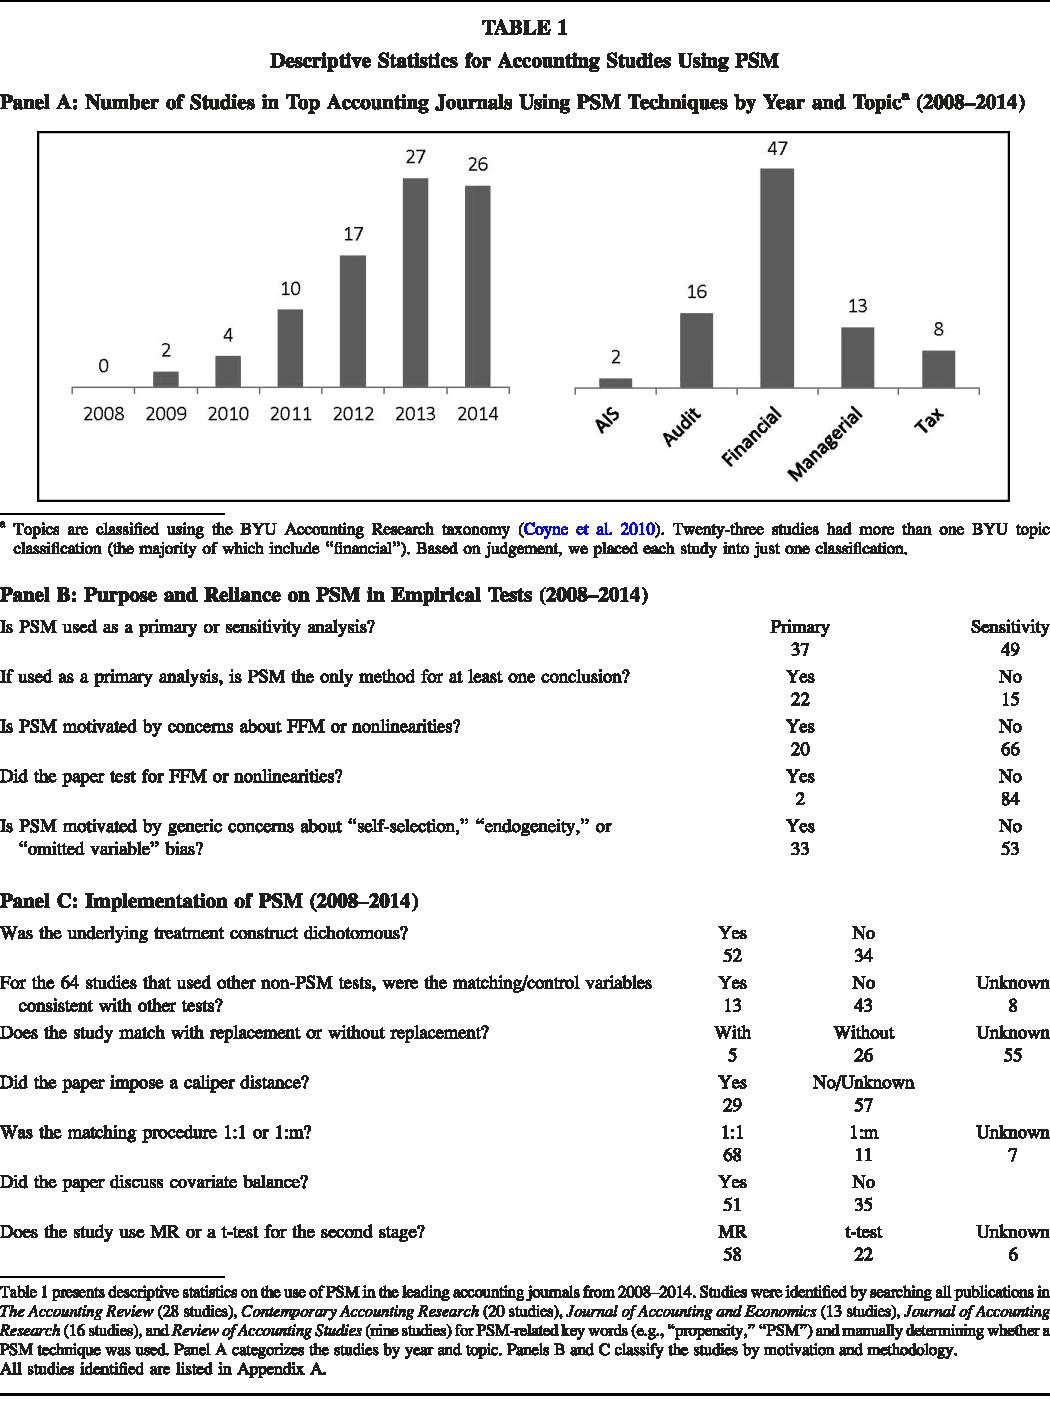
\includegraphics[width=16cm]{../table/tbl01.pdf}
\end{table}

\begin{itemize}
 \item 2008 $\sim$ 2014 年における、\textit{The Accounting Review,
       Contemporary Accounting Research, Journal of Accounting and
       Economics, Journal of Accounting Research, and Review of
       Accounting Studies} に掲載された論文延べ 86 件が対象。
 \item 会計研究で PSM が用いられはじめたのは最近 (86 件中 70 件は 2012
       $\sim$ 2014 の期間に刊行)。
\end{itemize}

\paragraph{各研究の PSM の位置付け (Table 1 Panel B)}

\begin{itemize}
 \item 主要な分析 (primary analyses) として用いている研究が 37 件である
       のに対し、ロバスト・チェック (sensitivity or robustness tests) と
       して用いている研究は 49 件。
 \item PSM を採用する理由として FFM や重回帰分析の線形性の仮定を挙げてい
       る研究はわずか 20 件。
 \item PSM が対処しうる内生性の問題を提示することなく、広く ``自己選択
       (self--selection),'' ``内生性 (endogeneity),'' および ``欠落変数
       バイアス (omitted variable bias)'' への対応として PSM を用いてい
       る研究が 33 件ある。
 \item Heckman (1979) の代わりとして誤用してしまっている研究も存在する。
\end{itemize}

\paragraph{処置群の選択の方法 (Table 1 Panel C)}

\begin{itemize}
 \item 問題の所在
       \begin{itemize}
        \item 処置が 2 値変数 (dichotomous) であるならば、PSM の実施は単純である。
        \item しかしながら、多様な状況でマッチングを実施するため、連続 (あるい
              は順序) 変数に閾値を設けて変換することがある\footnote{2 値
              変数を用いた処置群の選択について、例えば修正再表示のアナウ
              ンスメントや IFRS のアドプションがあげられる。一方で、非 2
              値変数を用いた処置群の選択について、企業の所有構造や監査人
              の産業特殊性 (auditor industry specialization) があげられ
              る}。
       \end{itemize}
 \item 問題点
       \begin{itemize}
        \item このような場合、閾値の近傍の観測値が over--represent される
              傾向があり、それによって、効果の大きさ (および平均処置効果)
              が消失し、第 II 種の過誤が生じる可能性が増大する。
       \end{itemize}
 \item 連続変数を用いている研究の数
       \begin{itemize}
        \item 34 件。また、この影響により、効果の大きさのみならずサンプ
              ル・サイズも低下する。
        \item 59 (12) 件の研究において、MR のサンプル・サイズの大きさは
              PSM の 3 (10) 倍である。
        \item サンプルサイズが小さいほど、サブサンプルは母集団を代表しな
              くなる。
       \end{itemize}
\end{itemize}

\paragraph{コントロール変数の選択 (Table 1 Panel C)}

\begin{itemize}
 \item MR と PSM のいずれを用いるにせよ、同様のコントロール変数を用いる
       べきであるにもかかわらず、しばしば異なるコントロール変数が用いら
       れていることがわかった。
 \item MR からマッチングに用いた変数を除外することは、その変数が処置変数
       (treatment) にも結果変数 (outcome) にも影響を与えないこと、
       ひいては、その変数によるマッチングが不必要であることを意味するに
       他ならない。
 \item 分析においては、\textit{post hoc} なモデルの特定 (model
       specification) をおこなっているという疑念 (appearance; 外観) を避
       けるため、PSM と他のテストとの説明変数の不一致を検討すべきである。
\end{itemize}

\paragraph{傾向スコア推定後のマッチング・プロシージャ (Table 1 Panel C)}

\begin{itemize}
 \item 置換処理 (replace)
       \begin{itemize}
        \item 55 件の研究において、マッチングに際して置換処理がおこなわ
              れているか否か (matching is performed with or without
              replacement) 開示されていない。
        \item 開示している 31 件の研究のうち、5 件が置換あり、26 件が置
              換なしであった。
       \end{itemize}
 \item キャリパー距離 (caliper distance)
       \begin{itemize}
        \item マッチング・プロシージャとしてキャリパー距離を開示して
              いる研究は 29 件のみ。
        \item 開示されているキャリパー距離の分布は、0.00005 から
              0.23 までで、よく用いられている距離は 0.01 (4 件)、0.03 (6
              件)、および 0.10 (5 件) である。
       \end{itemize}
 \item 1 対 1 と 1 対多のどちらのマッチングを用いるか
       \begin{itemize}
        \item 1 対 1 (one--to--one) が 68 instances であるのに対し、1 対
              多 (one--to--many) が 11 instances である。
       \end{itemize}
\end{itemize}

\paragraph{covariate balance (Table 1 Panel C)}

\begin{itemize}
 \item マッチング変数の数 (number of matching variables)、キャリパー距離
       (caliper distance)、グループ・サイズ (group size) などの要因は、
       PSM によってサンプルに covariate balance が生じる程度に影響する。
 \item しかしながら、covariate balance の決定はマッチング・クオリティ
       についての主観的な判断を要求するため、マッチングが実際に適切な
       (sufficient) balance を達成しているか否か、しばしば不透明である。
 \item サーベイの結果、35 件はマッチされたサンプル (matched sample) の
       covariate balance について議論しておらず、4 件のみ傾向スコ
       アの平均差について議論している。
 \item 研究においては、残存した covariate imbalance の効果を緩和するため
       に、PSM のサブサンプルにおいて MR を使うことができる。
 \item サーベイの結果、58 件は (第 2 段階の) ATE を推定する際に MR を用
       いている、22 件は結果変数の距離を t 検定することによって、処置効
       果を推定している、そして、6 件は推定手法を開示していないというこ
       とが明らかとなった。
\end{itemize}

\paragraph{サーベイの結論}

\begin{itemize}
 \item 本節で指摘した問題点は現在の文献でも改善されていない。
 \item Heckman (1979) モデルについて含意を示した Lennox et al. (2012,
       589) の結論と同様に、われわれは、多数の研究が ``重要な計量経済学
       上の問題点および PSM の利用をとりまく問題点に対する理解
       (appreciation) がほとんど無いままに、'' PSM を実施していると結論
       付ける。 
\end{itemize}
\section{EMPIRICAL EXAMPLES OF PROPENSITY SCORE MATICHNG IN ACCOUNTING SETTINGS}
監査法人の規模、内部統制、アナリストのフォロー数が財務報告の質に与える影響を検証する。

\subsection*{Sample Selection and Descriptive Statistics}

\paragraph{サンプルの選択}

\begin{itemize}
 \item 期間は、Sarbanes-Oxley (SOX) 法にかかる観測値が取得可能な2004〜2012年である。
 \item 以下の要件に該当するサンプルを除外する。
   \begin{itemize}
    \item 海外企業、および金融業(2桁SICコードの60--69)に属する観測値
    \item 総資産が500ドル以下の観測値
    \item 2桁SICコードに基づく産業年が10観測値未満のもの(裁量的会計発生高を計算するための要件)
    \item 欠損値のある観測値
   \end{itemize}
 \item 最終サンプルは、監査法人の規模の分析とアナリストのフォローの分析で29,227観測値、内部統制の弱さの分析で20,385観測値である。
 \item 最終サンプルの内訳は、以下のとおりである。
    \begin{itemize}
    \item Big 4に監査されている($\mathit{BIG}4_{it}=1$)のが19,988企業年
    \item 少なくとも1つの内部統制の弱さを監査報告書で指摘されている($\mathit{WEAK}_{it}=1$)のが1,422企業年
    \item 少なくとも1人のアナリストがついている($\mathit{ANALYST}_{it}=1$)21,144企業年
   \end{itemize}
\end{itemize}

\paragraph{データソース}

\begin{itemize}
 \item 監査法人、内部統制の弱さ、財務諸表の再報告にかかるデータ:Audit Analytics
 \item アナリストにかかるデータ:the Institutional Brokers’ Estimate System (I/B/E/S)
 \item 財務データ:Compustat
  \begin{itemize}
   \item Table 2:記述統計量
  \end{itemize}
\end{itemize}

\subsection*{Research Design}

$\mathit{BIG}4_{it}$、$\mathit{WEAK}_{it}$、$\mathit{ANALYST}_{it}$のそれぞれを割り当て変数とし、PSMを行い、ATEを推定する。

\paragraph{予測モデル(第1段階)}

\begin{equation}
\mathit{D}_{it} = \alpha_0 + \alpha_1 \mathit{X}_{it} + \varepsilon_{it}
\end{equation}

\begin{itemize}
 \item $\mathit{D}_{it}$は、$\mathit{BIG}4_{it}$、$\mathit{WEAK}_{it}$、$\mathit{ANALYST}_{it}$で、処置群と対照群に割り当てるダミー変数
 \item PSMのキャリパー距離は、0.03とする。
\end{itemize}

\paragraph{結果モデル(第2段階)}

\begin{equation}
\mathit{QUALITY}_{it} = \beta_0 + \beta_1 \mathit{D}_{it} + \beta_2 \mathit{X}_{it} +\varepsilon_{it}
\end{equation}

\begin{itemize}
 \item $\mathit{QUALITY}_{it}$は、財務報告の質を示し、本分析では、裁量的会計発生高($\mathit{ABSACC}_{it}$)、および財務諸表の再報告($\mathit{RESTATE}_{it}$)のそれぞれで評価している。
 \item $X_{it}$は、企業規模($\mathit{LNASSETS}_{it}$)、パフォーマンス($\mathit{ROA}_{it}$、$\mathit{ATURN}_{it}$)、財政状態($\mathit{CURR}_{it}$、$\mathit{LEV}_{it}$、$\mathit{DISTRESS}_{it}$)、設立年数($\mathit{AGE}_{it}$)、成長性($\mathit{GROWTH}_{it}$)、企業価値($\mathit{BTM}_{it}$)、年度固定効果を用いる。
  \begin{itemize}
   \item Appendix B:変数の定義
  \end{itemize}
 \item 本分析で観察したいATEは、(5)式の$\beta_1$で示される。
\end{itemize}

\subsection*{Diagnosing Function Form Misspecification}
\begin{itemize}
 \item MRにおいて、FFMが懸念されるのかについて判定する。
 \item Ramsey(1969)のRESETテストがFFMを見る手法として用いられることがある(Lawrence et al. 2011を見よ)。
 \item ただし、これは、変数の非線形性が追加的な説明を与えているのかどうかについて検証するものであり、結果変数と非線形な関係にある変数がATEの推定にバイアスを与えてるのかどうかを見るものではない。
\end{itemize}

\paragraph{変数を追加してFFMを判定する方法(Table 3)}

\begin{itemize}
 \item ここで、MRにおけるFFMを判定する手法として、コントロール変数(たとえば、変数を2乗したもの、3乗したもの)を追加する手法を提唱する。
 \item もし、元のモデルと変数を追加したモデルの結果が異なるのなら、FFMに対する懸念がある。
 \item (5)式を推定した結果を見ると、変数を追加したとしても((2)列と(5)列)、基本的な結果は元のモデル((1)列と(4)列)大きくは変わらない。
 \item しかし、監査法人の規模とアナリストのフォローで割り当てた場合、Chow(1960)の検定をすると、元のモデルのATEと変数を追加したモデルのATEの間で有意な差が認められる。
  \begin{itemize}
   \item これは、$X$と結果変数が非線形な関係にあることを示す。
  \end{itemize}
\end{itemize}

\subsection*{First-Stage Prediction Model}

\paragraph{第1段階((4)式)の推定結果(Table 4)}

\begin{itemize}
 \item 先行研究では、pseudo-${\rm R^2}$が高ければ高いほど、PSMは良い状態であることが示唆されている。
 \item しかし、この説明力は、割り当てが大きく影響を与えている。
 \item つまり、処置群の$X$が対照群の$X$とより大きく相違しているのなら、回帰式の説明力は大きくなる。
 \item overlapが大きければ大きいほど、pseudo-${\rm R^2}$は小さくなるとも言える。
  \begin{itemize}
   \item ただし、説明力がPSMの有効性を必ずしも示しているわけではない。
  \end{itemize}
\end{itemize}

\subsection*{Demonstration of Propensity Score Overlap}

処置群と対照群の傾向スコアのoverlapについて確認するため、Shaikh, Simonsen, Vydacil, and Yildiz(2009)と同様に、傾向スコアの密度をプロットする。

\paragraph{監査法人の規模で割り当てた場合の傾向スコアのプロット(Figure 1, Panel A)}

\begin{figure}
 \centering
 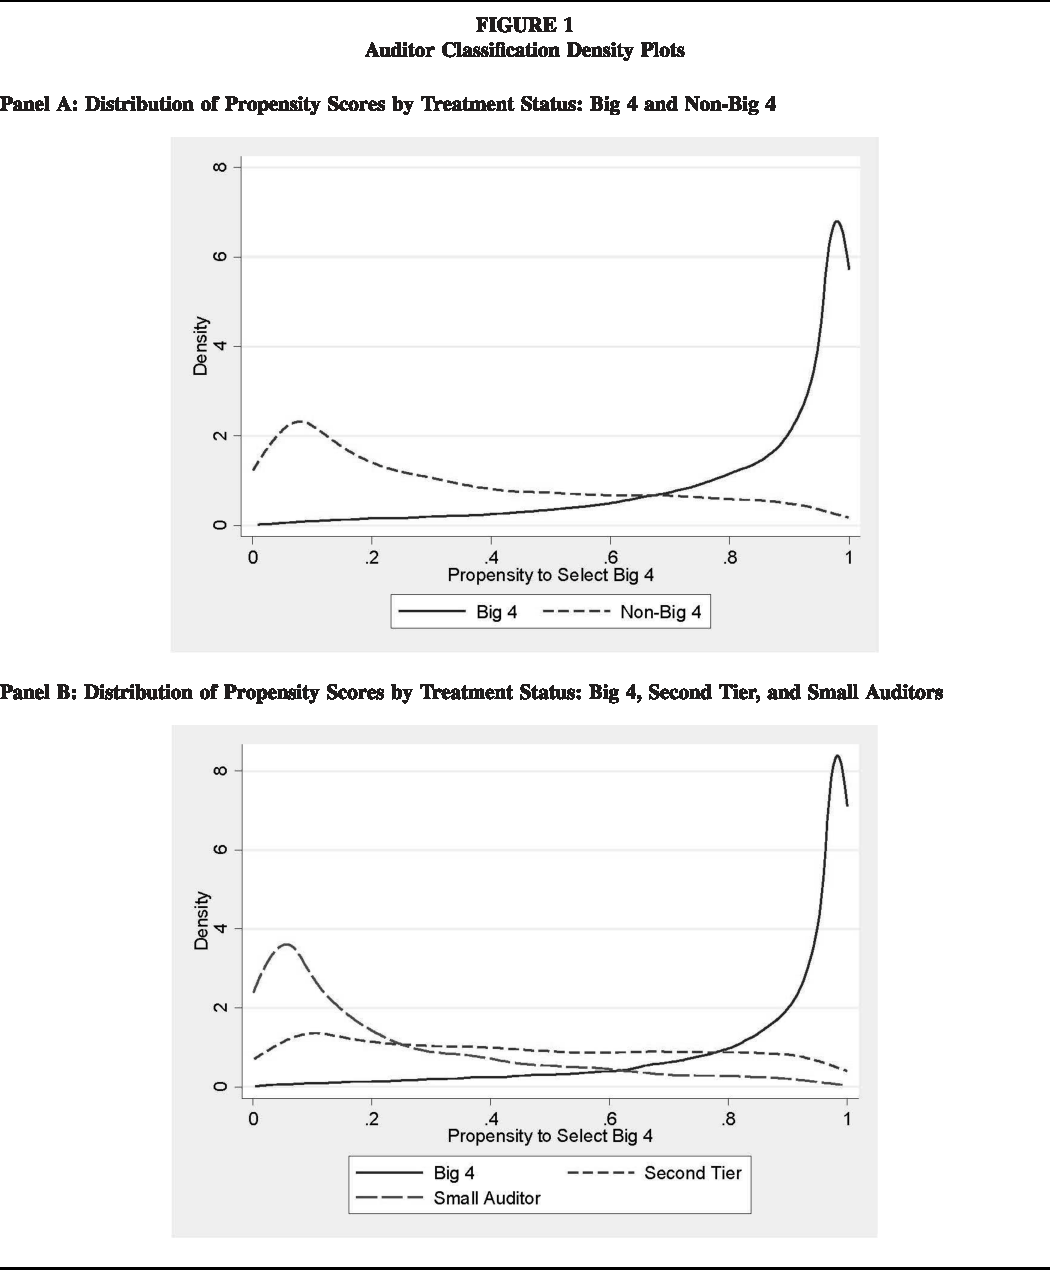
\includegraphics[width=16cm]{../fig/fig01.pdf}
\end{figure}

\begin{itemize}
 \item Big 4の監査法人のクライアントの傾向スコアは、0.9〜1の範囲内に集中し、非Big 4の監査法人のクライアントの傾向スコアは、0〜0.2に集中している。
 \item これは、共変量が割り当ての決定に大きく影響していることを示している。
 \item 結果的に、マッチングは、主として極端でない傾向スコアの範囲(ここでは、0.2〜0.9)の範囲内でなされることになる。
\end{itemize}

\paragraph{Second Tierを考慮して割り当てた場合の傾向スコアのプロット(Figure 1, Panel B)}

\begin{itemize}
 \item 非Big 4のクライアントから、Second Tierの監査法人のクライアントを識別する。
 \item この識別をしたプロットを見ると、Second Tierのクライアントは、0〜0.2の範囲内で、小規模監査法人のクライアントよりも傾向スコアが小さいが、0.2以上では小規模監査法人よりも大きな傾向スコアであることがわかる。
 \item これは、Second TierのクライアントがBig 4のクライアントとより多くマッチングが成立することを示す。
\end{itemize}

\paragraph{内部統制の弱さで割り当てた場合の傾向スコアの密度のプロット(Figure 2, Panel A)}

\begin{figure}
 \centering
 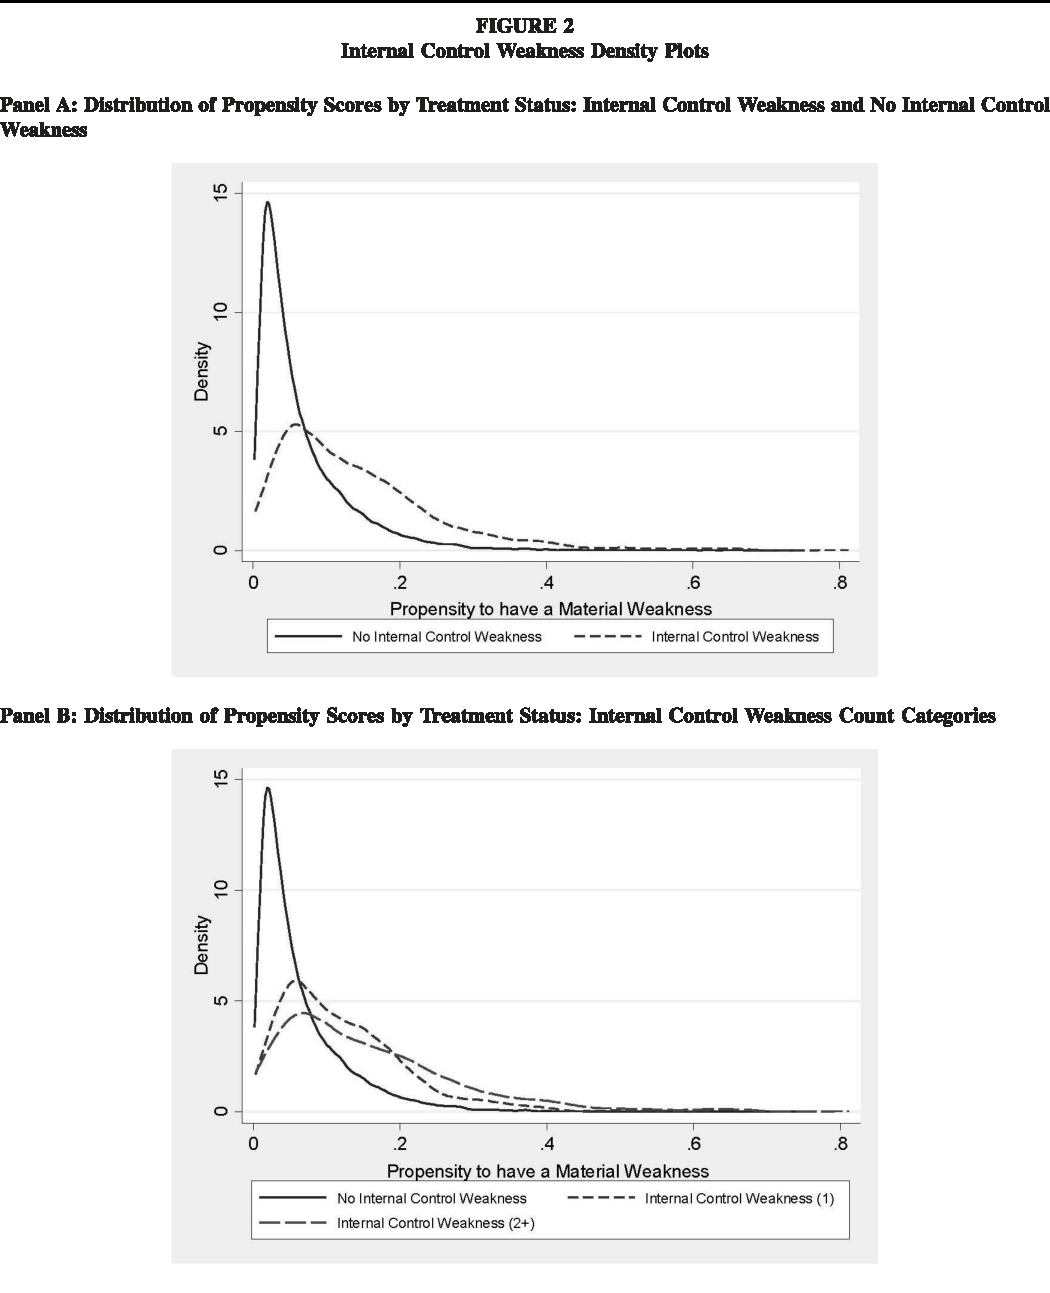
\includegraphics[width=16cm]{../fig/fig02.pdf}
\end{figure}

\begin{itemize}
 \item 監査法人の規模のときよりも、overlapの範囲が大きいことがわかる。
 \item Table 4のpseudo-${\rm R^2}$も、低い値であることもこのことを示唆している。
\end{itemize}

\paragraph{内部統制の弱さの判定を詳細にした場合の傾向スコアの密度のプロット(Figure 2, Panel B)}

\begin{itemize}
 \item 内部統制の弱さの判定をより詳細にする(No ICW、1 ICW、2+ICW)。
 \item 監査法人の規模の場合と同様に、overlapは、No ICWと2+ICWの間よりも、No ICWと1 ICWの間の方がより大きいことがわかる。
\end{itemize}

\paragraph{アナリストのフォローで割り当てた場合の傾向スコアの密度のプロット(Figure 3, Panel A)}

\begin{itemize}
 \item 監査法人の場合と同様に、処置群と対照群との間で傾向スコアの密度の範囲は異なっており、overlapが限定的なものであることがわかる。
\end{itemize}

\paragraph{アナリストのフォロー数を詳細にした場合の傾向スコアの密度のプロット(Figure 3, Panel B)}

\begin{itemize}
 \item アナリストのフォロー数を詳細にみる(1〜5人、6〜10人、11人以上)。
 \item プロットした結果、アナリストの数が少なければ少ないほど、アナリストに全くフォローされてない観測値とのoverlapが大きくなることがわかる。
 \item これは、マッチングがフォローしているアナリストの数の少ない企業となされる可能性が高いことを示している。
\end{itemize}

\subsection*{Matching without Replacement}

置き換えを認めず、1対1でマッチングを行う。

\paragraph{サンプルの構成(Table 5, Panel A)}

\begin{itemize}
 \item 置き換えをせず1対1でマッチングすると、かなりの数の観測値を除去することになる。
 \item 事実、“full sample”を比較して、監査法人の規模で30\%、内部統制の弱さで14\%、アナリストのフォローで28\%のサンプルしか確保できなかった。
 \item また、マッチングしたサンプルは、Second Tierのクライアントや、アナリストのフォロー数が少ない観測値で構成されていることもわかる。
  \begin{itemize}
   \item サンプルが小さいことは、外的な妥当性を減少させる、もしくは欠落させてしまう可能性を有している。
  \end{itemize}
\end{itemize}

\paragraph{MRとPSM間における共変量とATEの比較(Table 5, Panel B)}

\begin{itemize}
 \item 共変量は、PSMを行うことにより、バランスが向上していることがわかる。
  \begin{itemize}
   \item これは、MRにおいて、処置群と対照群の相違が残ったまま、ATEを推定していることを示す。
  \end{itemize}
 \item 裁量的会計発生高を従属変数とした場合、MRのATEはすべて有意であるが、PSMはすべて非有意であり、Chow(1960)の検定も、すべての係数間で有意である。
 \item 一方、財務諸表の再報告を従属変数とした場合は、MRとPSMのATEともにすべて類似した結果を示すが、係数を比較すると、有意な差が検出されるものが存在している。
\end{itemize}

\paragraph{まとめ}
\begin{itemize}
 \item 以上の分析から、MRとPSMでは推定される ATEが有意に異なっていることが明らかとなった。
 \item もし、PSMのみで分析すると、監査法人の規模、内部統制の弱さ、およびアナリストのフォローは、財務報告の質に影響を与えていないという結果のみを得ることになる。
 \item しかし、この ``帰無仮説を採択する'' (accept the null hypothesis) のは結論を急ぎ過ぎ (premature) であるかもしれない。
 \item 以下で、PSMの手法を変更することで、結果が変化することを示す。
\end{itemize}

\subsection*{Matching with Replacement}

置き換えを認めて、1対1でマッチングを行う。

\paragraph{サンプルの構成(Table 6, Panel B)}

\begin{itemize}
 \item (2)列目は、サンプルサイズが小さい方の群を処置群とし、サンプルサイズの大きな方の群にマッチングの置き換えを認める場合の結果である(Panel A)。
 \item サンプルサイズが大きくなっており、キャリパー距離(0.03)の間でより多くの対照群の観測値がマッチングしていることがわかる。
 \item (3)列目は、サンプルサイズの大きな方の群を処置群とし、サンプルサイズの小さい方の群にマッチングの置き換えを認める場合の結果である。
 \item サンプルサイズがかなり大きくなっており、ウェイトがいずれも5以上であることから、対照群の観測値がより多くの回数マッチングしていることがわかる。
 \item マッチングの手法ごとにサンプルの構成を比較した結果、9個の比較中8個で有意な差が認められる。
 \item 特に、Second Tierのクライアントの割合と、アナリストのフォロー数の平均値は、マッチングの手法間で顕著な差がある。
  \begin{itemize}
   \item マッチング手法の違いが、サンプルサイズとサンプルの構成に影響を与えてしまうことが示唆されている。
  \end{itemize}
\end{itemize}

\paragraph{ATEの比較(Table 6, Panel B, C)}

\begin{itemize}
 \item 監査法人の規模で割り当てた場合の結果は、いずれも非有意である。
 \item しかし、ATEの差が有意に検出されているものが存在する(6個の比較中3個)。
 \item 内部統制の弱さ、およびアナリストのフォローで割り当てた場合の結果は、マッチングの手法ごとに異なっており、ATEの差も有意に検出されているものがある(12個の比較中7個)。
  \begin{itemize}
   \item マッチングの手法が統計的な結果に影響を与えてしまう。
  \end{itemize}
\end{itemize}

\subsection*{The Influence of Matching Variables on Estimates of the ATE}

\paragraph{変数を置き換えてマッチングを行なった場合のサンプルの構成(Table 7, Panel A)}

\begin{itemize}
 \item 企業規模を示す変数を、総資産の自然対数($\mathit{LNASSETS}_{it}$)から時価総額の自然対数($\mathit{LNMARKET}_{it}$)に入れ替える。
 \item マッチングの手法間でサンプルを比較すると、共通の観測値は、58.9〜71.4\%の割合である。
 \item さらに、内部統制の弱さで割り当てた場合の対照群(内部統制の弱さが指摘されていない観測値)は、マッチングの手法間で、わずか18.2\%しかサンプルが共通してない。
\end{itemize}

\paragraph{変数を置き換えてマッチングを行なった場合のATE(Table 7, Panel B)}

\begin{itemize}
 \item $\mathit{LNASSETS}_{it}$のATEよりも、$\mathit{LNMARKET}_{it}$のATEの方が、有意であるものが多いことがわかる。
 \item 特に、アナリストのフォローで割り当てとし、財務諸表の再報告を従属変数とした時のATEは、Table 5の全サンプルとマッチングサンプルで非有意だったにもかかわらず、変数を置き換えると有意な結果が確認される。
 \item Chow(1960)の検定によれば、6個の比較中、3個でATEが有意な差であることが確認される。
\end{itemize}

\paragraph{変数を追加してマッチングを行った場合の結果(Table 8)}

\begin{itemize}
 \item 以下のとおり、変数を追加してマッチングを行う。
  \begin{itemize}
   \item 監査法人の規模:営業活動にかかるキャッシュフロー($\mathit{CFO}_{it}$)、海外売上高($\mathit{FOREIGN}_{it}$)
   \item 内部統制の弱さ:損失ダミー($\mathit{LOSS}_{it}$)
   \item アナリストのフォロー:$\mathit{LNMARKET}_{it}$
  \end{itemize}
 \item このマッチングからATEを求めた結果は、(2)列目と(5)列目に示されているが、いずれも有意であることがわかる。
 \item さらに以下のとおり変数を追加する。
  \begin{itemize}
   \item 監査法人の規模:$\mathit{LNASSETS}_{it-1}$、$LOSS_{it}$、棚卸資産($\mathit{INVENTORY}_{it}$)
   \item 内部統制の弱さ:$\mathit{FOREIGN}_{it}$
   \item アナリストのフォロー:$\mathit{BTM}_{it-1}$
  \end{itemize}
 \item 以上でマッチングし、ATEを求めた結果は、(3)列目と(6)列目に示されているが、これまでの検証で一貫して有意である内部統制の弱さで割り当て、財務諸表の再報告を従属変数としたATE以外、すべて非有意である。
  \begin{itemize}
   \item 以上から、ATEの推定は、PSMのモデルの設定から影響を受けやすいことが明らかである。
  \end{itemize}
 \item 以上の変数の選択は、結果の頑健性を示すために、``事後的''に選択されたことに留意するべきである。
 \item すべての$X$は、結果に同じような影響を与えるとは限らない。
  \begin{itemize}
   \item ここから、PSMの変数の選択において、十分な考慮をするこの重要さが示唆される。
  \end{itemize}
\end{itemize}

\section{CONCLUSION}

\begin{itemize}
 \item Shipman, Swanquist, and Whited の分析対象
       \begin{itemize}
        \item PSM の理論的基礎を議論し、昨今の会計研究における PSM の利
              用を調査し、そして、デザインの選択 (design choice) にかん
              する実践的なインプリケーションを例示した。
       \end{itemize}
 \item 会計研究における PSM の利用 (第 3 節) の要約
       \begin{itemize}
        \item 観察不能なデータによって生じる内生性を緩和するための
              Heckman (1979) モデルの代わりとして、誤って利用しているケー
              スがしばしば確認される。
        \item デザインの選択を開示していない、あるいは、PSM と MR とでコ
              ントロール変数が不一致である研究が散見される。
       \end{itemize}
 \item デザインの選択 (第 4 節) の要約
       \begin{itemize}
        \item カットオフ・ポイント (cutoff point) が処置群を決定する場合、
              カットオフの近傍の観測値は over--represent し、第 II 種の
              過誤が生じる可能性が増大する。
        \item PSM による推定は変化しやすく (fickle) リプリケートが難しい
              ため、マッチド・サンプルに対して ``ストレス・テスト''
              (stress testing) を実施し、また、代替的なリサーチ・デザイ
              ンで PSM の追加検証を実施することが要求される。
       \end{itemize}
 \item 将来研究への提言
       \begin{itemize}
        \item 重要なデザインの選択を開示すること。
        \item PSM の利用目的を適切に理解すること。
        \item マッチド・サンプル以外の specification concerns も調査する
              こと。
        \item PSM に対して他のリサーチ・デザインをもとに追加分析を実施す
              ること、および、FFM に対処する新たな手法を模索すること。
       \end{itemize}
\end{itemize}
\appendix
\setcounter{section}{1}
\section{Appendix B}
\begin{longtable}[c]{ll}
 \caption{Variable Descriptions}
 \label{tab:appB}
 \\
 % -- ページの表の最上部 --
 \hline
  Variable Name & \hspace{5cm} Variable Definition \\ \hline
 \endhead
 % -- ページの表の最下部 --
 \hline
 \endfoot
 % ------------------------
  $\text{ABSACC}_{it}$ & 全ての産業--年度において最低10個の観測値をもとに以下の回帰式を推定し、\\
  & 得られた誤差を業績とマッチさせて算定した裁量的会計発生高 \vspace{0.5cm} \\
  \vspace{0.3cm}
  & {$\!
      \begin{aligned}
     \frac{TA}{A} = \alpha + \lambda_{0} 
       \frac{1}{A} + \lambda_{1} \frac{\Delta REV - \Delta REC}{A} 
       + \lambda_{2}\frac{PPE}{A}
      \end{aligned} $} \\
  & \begin{tabular}{ll} \hline
     $A$ & 総資産の平均値 \\
     $\text{TA}$ & 総会計発生高 (= 経常利益 - 営業活動によるキャッシュ・フロー) \\
     $\Delta REV$ & 売上高の変化額 \\
     $\Delta REC$ & 売上債権の変化額 \\
     $PPE$ & 有形固定資産 \\ \hline
    \end{tabular} \vspace{0.3cm} \\ 
  & 上記の回帰式から得られた各観測値の誤差を、\\
  & 同じSIC (two-digit) コードでROAが最も近似している観測値から引いた絶対値を \\
  & $\text{ABSACC}$ としている。\\
  $\text{ANALYST}_{it}$ & 1人以上のアナリストがフォローしている企業であれば1、\\
  & そうでなければ0を与えるダミー変数 \\
  $\text{AGE}_{it}$ & t年時点でCompustatに収録されている企業年数 \\
  $\text{ATURN}_{it}$ & 売上高÷総資産の平均値 \\
  $\text{BIG4}_{it}$ & 監査人が4大監査法人であれば1、そうでなければ0を与えるダミー変数\\
  $\text{BTM}_{it}$ & 簿価時価比率 \\
  $\text{CFO}_{it}$ & 営業活動によるキャッシュ・フロー÷総資産額の平均値\\
  $\text{CURR}_{it}$ & 流動比率\\
  $\text{DISTRESS}_{it}$ & Altman (1983) に基づいて算定したZスコア\\
  & {$\!
      \begin{aligned}
       0.717 \times \frac{\text{運転資本}}{\text{総資産}} &+ 0.847 \times \frac{\text{留保利益}}{\text{総資産}} 
       + 3.107 \times \frac{\text{利息・税控除前利益}}{\text{総資産}} \\
       &+ 0.42 \times \frac{\text{自己資本簿価}}{\text{総負債}}
       + 0.998 \times \frac{\text{売上高}}{\text{総資産}}
      \end{aligned} $} \\
  $\text{FOREIGN}_{it}$ & 外国為替損益が0でなければ1、そうでなければ0を与えるダミー変数 \\
  $\text{GROWTH}_{it}$ & t-1期からt期への売上高の変化額÷t-1時点の売上高 \\
  $\text{INVENTORY}_{it}$ & 棚卸資産÷総資産\\
  $\text{LEV}_{it}$ & 長期借入金 (long-term debt) と短期借入金の合計額÷総資産 \\
  $\text{LNASSETS}_{it}$ & 総資産額 (単位: 100万) の自然対数 \\
  $\text{LNMARKET}_{it}$ & 時価総額 (単位: 100万) の自然対数 \\
  $\text{LOSS}_{it}$ & operating income after depreciationが\\ 
  & マイナスであれば1、そうでなければ0を与えるダミー変数 \\
  $\text{RESTATE}_{it}$ & t期の財務諸表について、後に訂正財務諸表を提出していれば1、\\
  & そうでなければ0を与えるダミー変数 \\
  $\text{ROA}_{it}$ & 当期純利益÷総資産の平均値\\
  $\text{WEAK}_{it}$ & 監査報告書において、内部統制に関する脆弱性が1点以上指摘されていれば1、\\
  & そうでなければ0を与えるダミー変数\\ 
\end{longtable}
\bibliography{./bib/myrefs}
\end{document}
